\documentclass[11pt,a4paper]{article}
\usepackage[utf8]{inputenc}
\usepackage{lmodern}
\usepackage[T1]{fontenc}
\usepackage[french]{babel}
\usepackage{amsmath,amssymb}
\usepackage{graphicx}
\usepackage{subcaption}
\usepackage{booktabs}
\usepackage[margin=2cm]{geometry}
\usepackage{fancyhdr}

\graphicspath{{fig/}}

\pagestyle{fancy}
\fancyhf{}
\fancyhead[L]{ETE7-TSIG2}
\fancyhead[R]{Cirou -- Païtard}
\fancyfoot[C]{\thepage}
\renewcommand{\headrulewidth}{0.4pt}

\begin{document}

\begin{titlepage}
  \centering
  {\large ENSEIRB-MATMECA}\\[0.2cm]
  {\large Filière Télécommunications -- 2\textsuperscript{e} année}\\[0.2cm]
  {\large ETE7-TSIG2 : Filtres numériques, estimation et applications}\\[3cm]

  \rule{\linewidth}{0.5pt}\\[0.4cm]
  {\LARGE\bfseries Rapport Projet Signaux}\\[0.3cm]
  {\large Extraction de marqueurs en vue d'une classification de signaux}\\
  \rule{\linewidth}{0.5pt}\\[3cm]

  {\large Marco \textsc{Cirou} \quad -- \quad Maxence \textsc{Païtard}}\\[1cm]
  {\large Encadrant : Éric \textsc{Grivel}}

  \vfill
  {\large Novembre 2026}
\end{titlepage}

\tableofcontents
\newpage

%=====================================================================
\section{Introduction}
%=====================================================================

La classification automatique de signaux, qu'il s'agisse de signaux biomédicaux, de parole ou de signaux radar, s'appuie rarement sur les échantillons bruts. Elle exploite des \emph{marqueurs}, c'est-à-dire des grandeurs scalaires qui résument une propriété statistique du signal et qui doivent rester stables d'une réalisation à l'autre pour une même classe. Ce projet porte sur l'extraction de l'un de ces marqueurs : la pente de la loi d'évolution, en échelle logarithmique, de la puissance d'un signal intégré puis privé de sa tendance, en fonction de la taille de la fenêtre d'analyse. Cette démarche est connue sous le nom d'analyse des fluctuations redressées (\emph{Detrended Fluctuation Analysis}, DFA)~[5].

La mise en œuvre de cette méthode fait appel aux notions de processus aléatoires, d'estimation et de filtrage numérique vues en cours. La section~\ref{sec:signaux} est consacrée aux signaux aléatoires : deux processus de référence, à moyenne mobile et autorégressif, sont générés et caractérisés par leur densité spectrale de puissance (DSP), puis comparés à quatre estimateurs non paramétriques de celle-ci. La section~\ref{sec:methode} détaille les quatre étapes de la méthode et justifie les choix d'estimation de la tendance : régression polynomiale par blocs, filtrage causal et filtrage à phase nulle. La section~\ref{sec:applications} applique la méthode à un bruit blanc et à un processus autorégressif d'ordre 2 et discute la robustesse du marqueur. Le rapport se termine par une conclusion technique et par le bilan de l'organisation du projet.

%=====================================================================
\section{Signaux aléatoires}
\label{sec:signaux}
%=====================================================================

Dans toute cette section, $u(n)$ désigne un bruit blanc gaussien centré de variance $\sigma_u^2 = 1$, et chaque réalisation comporte $N = 2000$ échantillons. Les fréquences $\nu = f/f_e$ sont normalisées par la fréquence d'échantillonnage $f_e$ et prises dans $[-1/2, 1/2[$.

\subsection{Processus à moyenne mobile d'ordre 4}

Pour obtenir des réjections spectrales aux fréquences normalisées $1/4$ et $4/9$ sur $[0, 1/2]$, le bruit $u(n)$ est filtré par un filtre dont les quatre zéros, de module $R = 0{,}95$, sont placés aux fréquences $\nu_k \in \{\pm 1/4, \pm 4/9\}$ : $z_k = R\, e^{j2\pi\nu_k}$. Les zéros étant deux à deux conjugués, les coefficients du filtre sont réels :
\begin{equation}
  B(z) = \prod_{k=1}^{4} \left( 1 - z_k\, z^{-1} \right) = \sum_{i=0}^{4} b_i z^{-i},
  \qquad
  x(n) = \sum_{i=0}^{4} b_i\, u(n-i),
  \label{eq:ma4}
\end{equation}
avec $b_0 = 1$, $b_1 \approx 1{,}785$, $b_2 \approx 1{,}805$, $b_3 \approx 1{,}611$ et $b_4 \approx 0{,}815$. La sortie ne dépend que d'un nombre fini d'échantillons d'entrée : le filtre est à réponse impulsionnelle finie (RIF) et $x(n)$ est un \emph{processus à moyenne mobile d'ordre 4}, noté MA(4).

Sa moyenne est nulle, $\mathbb{E}[x(n)] = \sum_i b_i\, \mathbb{E}[u(n-i)] = 0$, et son autocorrélation ne dépend que du décalage $k$ :
\begin{equation}
  r_x(k) = \mathbb{E}[x(n)x(n-k)] =
  \begin{cases}
    \sigma_u^2 \displaystyle\sum_{i=0}^{4-|k|} b_i\, b_{i+|k|} & \text{si } |k| \leq 4,\\[2mm]
    0 & \text{si } |k| > 4.
  \end{cases}
  \label{eq:r_ma}
\end{equation}
Le processus est donc stationnaire au sens large (SSL), de variance $r_x(0) = \sigma_u^2 \sum_i b_i^2 \approx 10{,}7$. La DSP s'écrit :
\begin{equation}
  S_x(\nu) = \sigma_u^2 \left| B\!\left(e^{j2\pi\nu}\right) \right|^2.
  \label{eq:dsp_ma}
\end{equation}
Les zéros étant proches du cercle unité sans être dessus, $S_x$ présente des creux marqués en $\pm 1/4$ et $\pm 4/9$ sans s'annuler : ils atteignent respectivement $-32$~dB et $-41$~dB par rapport au maximum, situé en $\nu = 0$ (figure~\ref{fig:dsp_ma}).

\subsection{Processus autorégressif d'ordre 4}

De manière analogue, le bruit $u(n)$ est filtré par un filtre dont les quatre pôles, de module $r = 0{,}99$, s'écrivent $p_k = r\, e^{j2\pi\nu_k}$ avec $\nu_k \in \{\pm 1/3, \pm 3/7\}$ :
\begin{equation}
  H(z) = \frac{1}{\prod_{k=1}^{4} \left( 1 - p_k\, z^{-1} \right)} = \frac{1}{1 + \sum_{i=1}^{4} a_i z^{-i}},
  \qquad
  x(n) = u(n) - \sum_{i=1}^{4} a_i\, x(n-i).
  \label{eq:ar4}
\end{equation}
L'échantillon $x(n)$ dépend de ses quatre échantillons passés : il s'agit d'un \emph{processus autorégressif d'ordre 4}, noté AR(4). Le filtre est à réponse impulsionnelle infinie (RII) ; sa stabilité n'est donc pas acquise par construction, mais elle est assurée ici car tous les pôles sont à l'intérieur du cercle unité ($r < 1$). La moyenne reste nulle et, en régime permanent, l'autocorrélation vérifie les équations de Yule-Walker, $r_x(k) = -\sum_{i=1}^{4} a_i\, r_x(k-i)$ pour $k \geq 1$ : elle n'est plus nulle au-delà d'un certain rang mais décroît comme $r^{|k|}$. La DSP s'écrit, par analogie avec~\eqref{eq:dsp_ma} :
\begin{equation}
  S_x(\nu) = \frac{\sigma_u^2}{\left| A\!\left(e^{j2\pi\nu}\right) \right|^2},
  \qquad A(z) = 1 + \sum_{i=1}^{4} a_i z^{-i}.
  \label{eq:dsp_ar}
\end{equation}
Les creux du cas MA laissent place à des pics de résonance en $\pm 1/3$ et $\pm 3/7$, et la DSP couvre une dynamique de $64$~dB (figure~\ref{fig:dsp_ma}).

Le processus n'est toutefois SSL qu'\emph{asymptotiquement} : le régime transitoire dû aux conditions initiales nulles décroît comme $r^n$, avec une constante de temps $1/(1-r) = 100$ échantillons. Il aurait fallu écarter environ $5/(1-r) = 500$ échantillons, ce qui n'a pas été fait dans le code ; la figure~\ref{fig:temporel} ne montre cependant pas d'enveloppe croissante en début de signal.

\subsection{Représentations temporelles et spectre de puissance}

La figure~\ref{fig:temporel} présente une réalisation de chaque processus. Le MA(4), dont la DSP est maximale à basse fréquence, varie relativement lentement ; son amplitude, de l'ordre de $\pm 10$, est cohérente avec un écart-type de $\sqrt{10{,}7} \approx 3{,}3$. L'AR(4) oscille rapidement, à des périodes de 3 et $7/3$ échantillons, et son enveloppe fluctue lentement par bouffées d'une centaine d'échantillons. Ces bouffées ne traduisent pas une non-stationnarité : elles sont la signature d'un processus à bande étroite, dont le temps de corrélation est de l'ordre de $1/(1-r) = 100$ échantillons.

\begin{figure}[!htb]
  \centering
  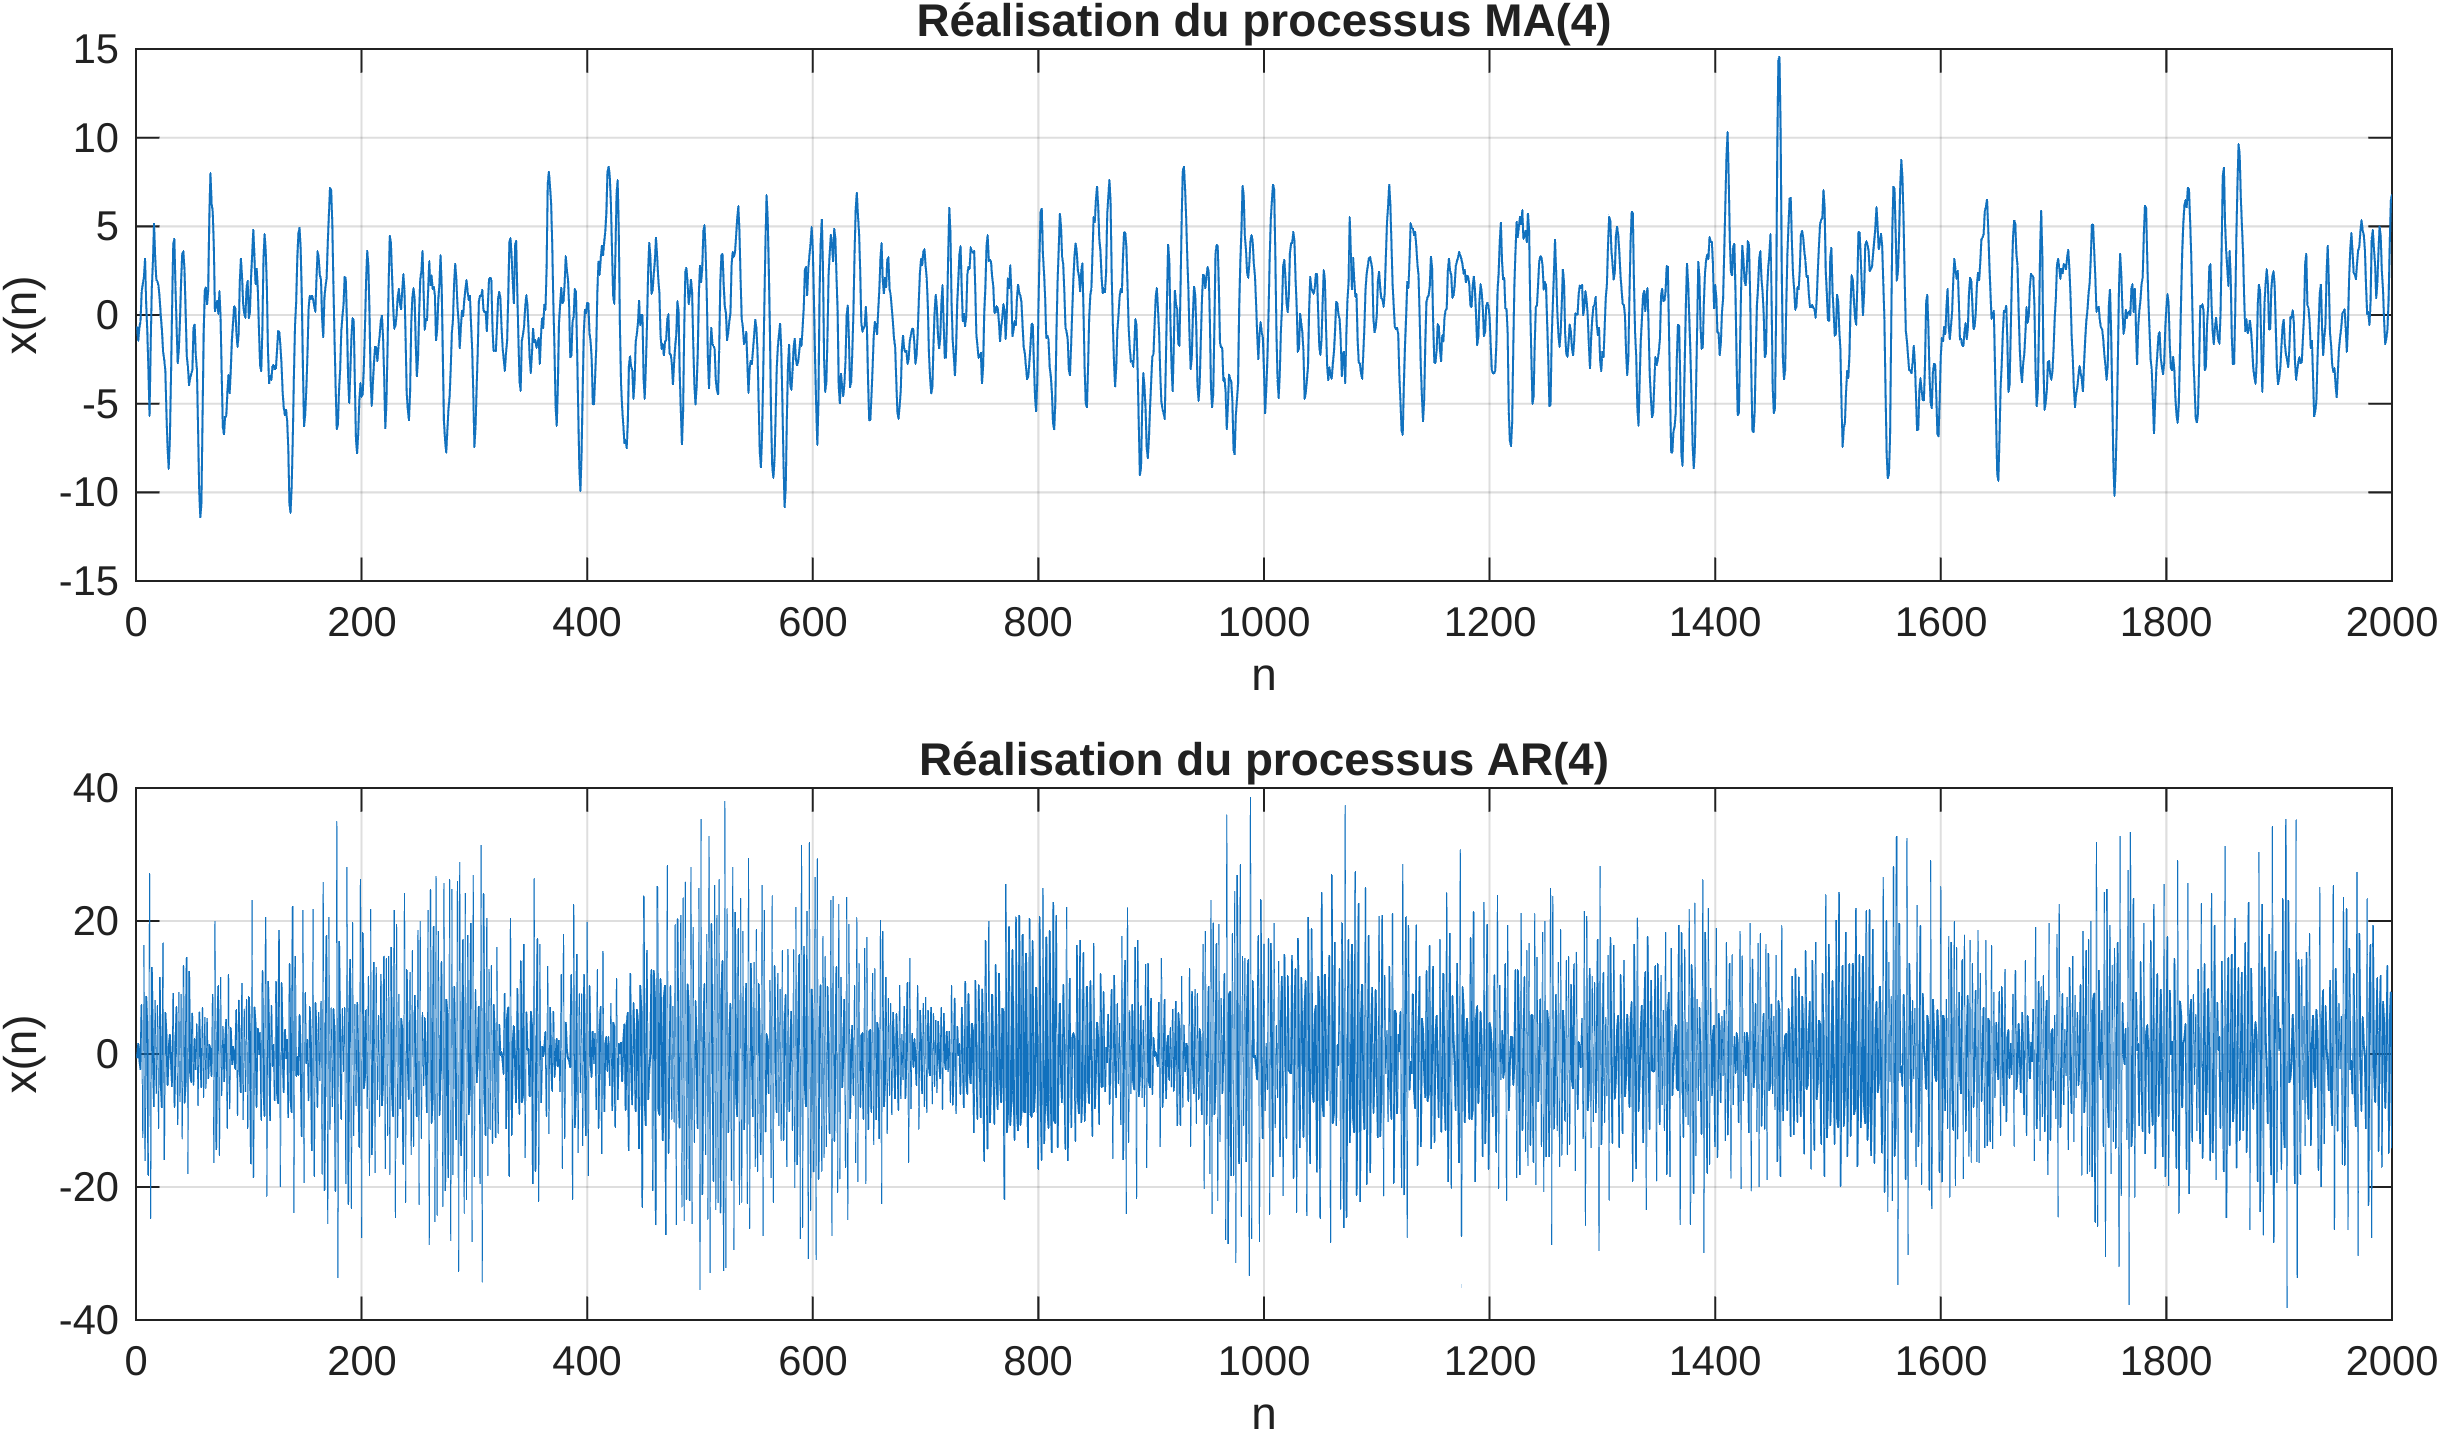
\includegraphics[width=0.72\linewidth]{fig04.png}
  \caption{Réalisations de $N = 2000$ échantillons des processus MA(4) (haut) et AR(4) (bas).}
  \label{fig:temporel}
\end{figure}

Il faut distinguer la DSP, grandeur théorique attachée au processus, du \emph{spectre de puissance} $|X(\nu)|^2/N$ calculé sur une seule réalisation. Sur la figure~\ref{fig:dsp_ma}, le spectre de puissance suit la forme de la DSP mais fluctue fortement autour d'elle. Sur le MA(4), il apparaît en outre décalé de 8 à 10~dB vers le bas : chaque courbe étant normalisée par son propre maximum, celle du spectre de puissance l'est par une valeur aléatoire particulièrement grande. Une normalisation par $\sigma_u^2$, connu ici, aurait permis une comparaison en niveau absolu.

\begin{figure}[!htb]
  \centering
  \begin{subfigure}{0.43\linewidth}
    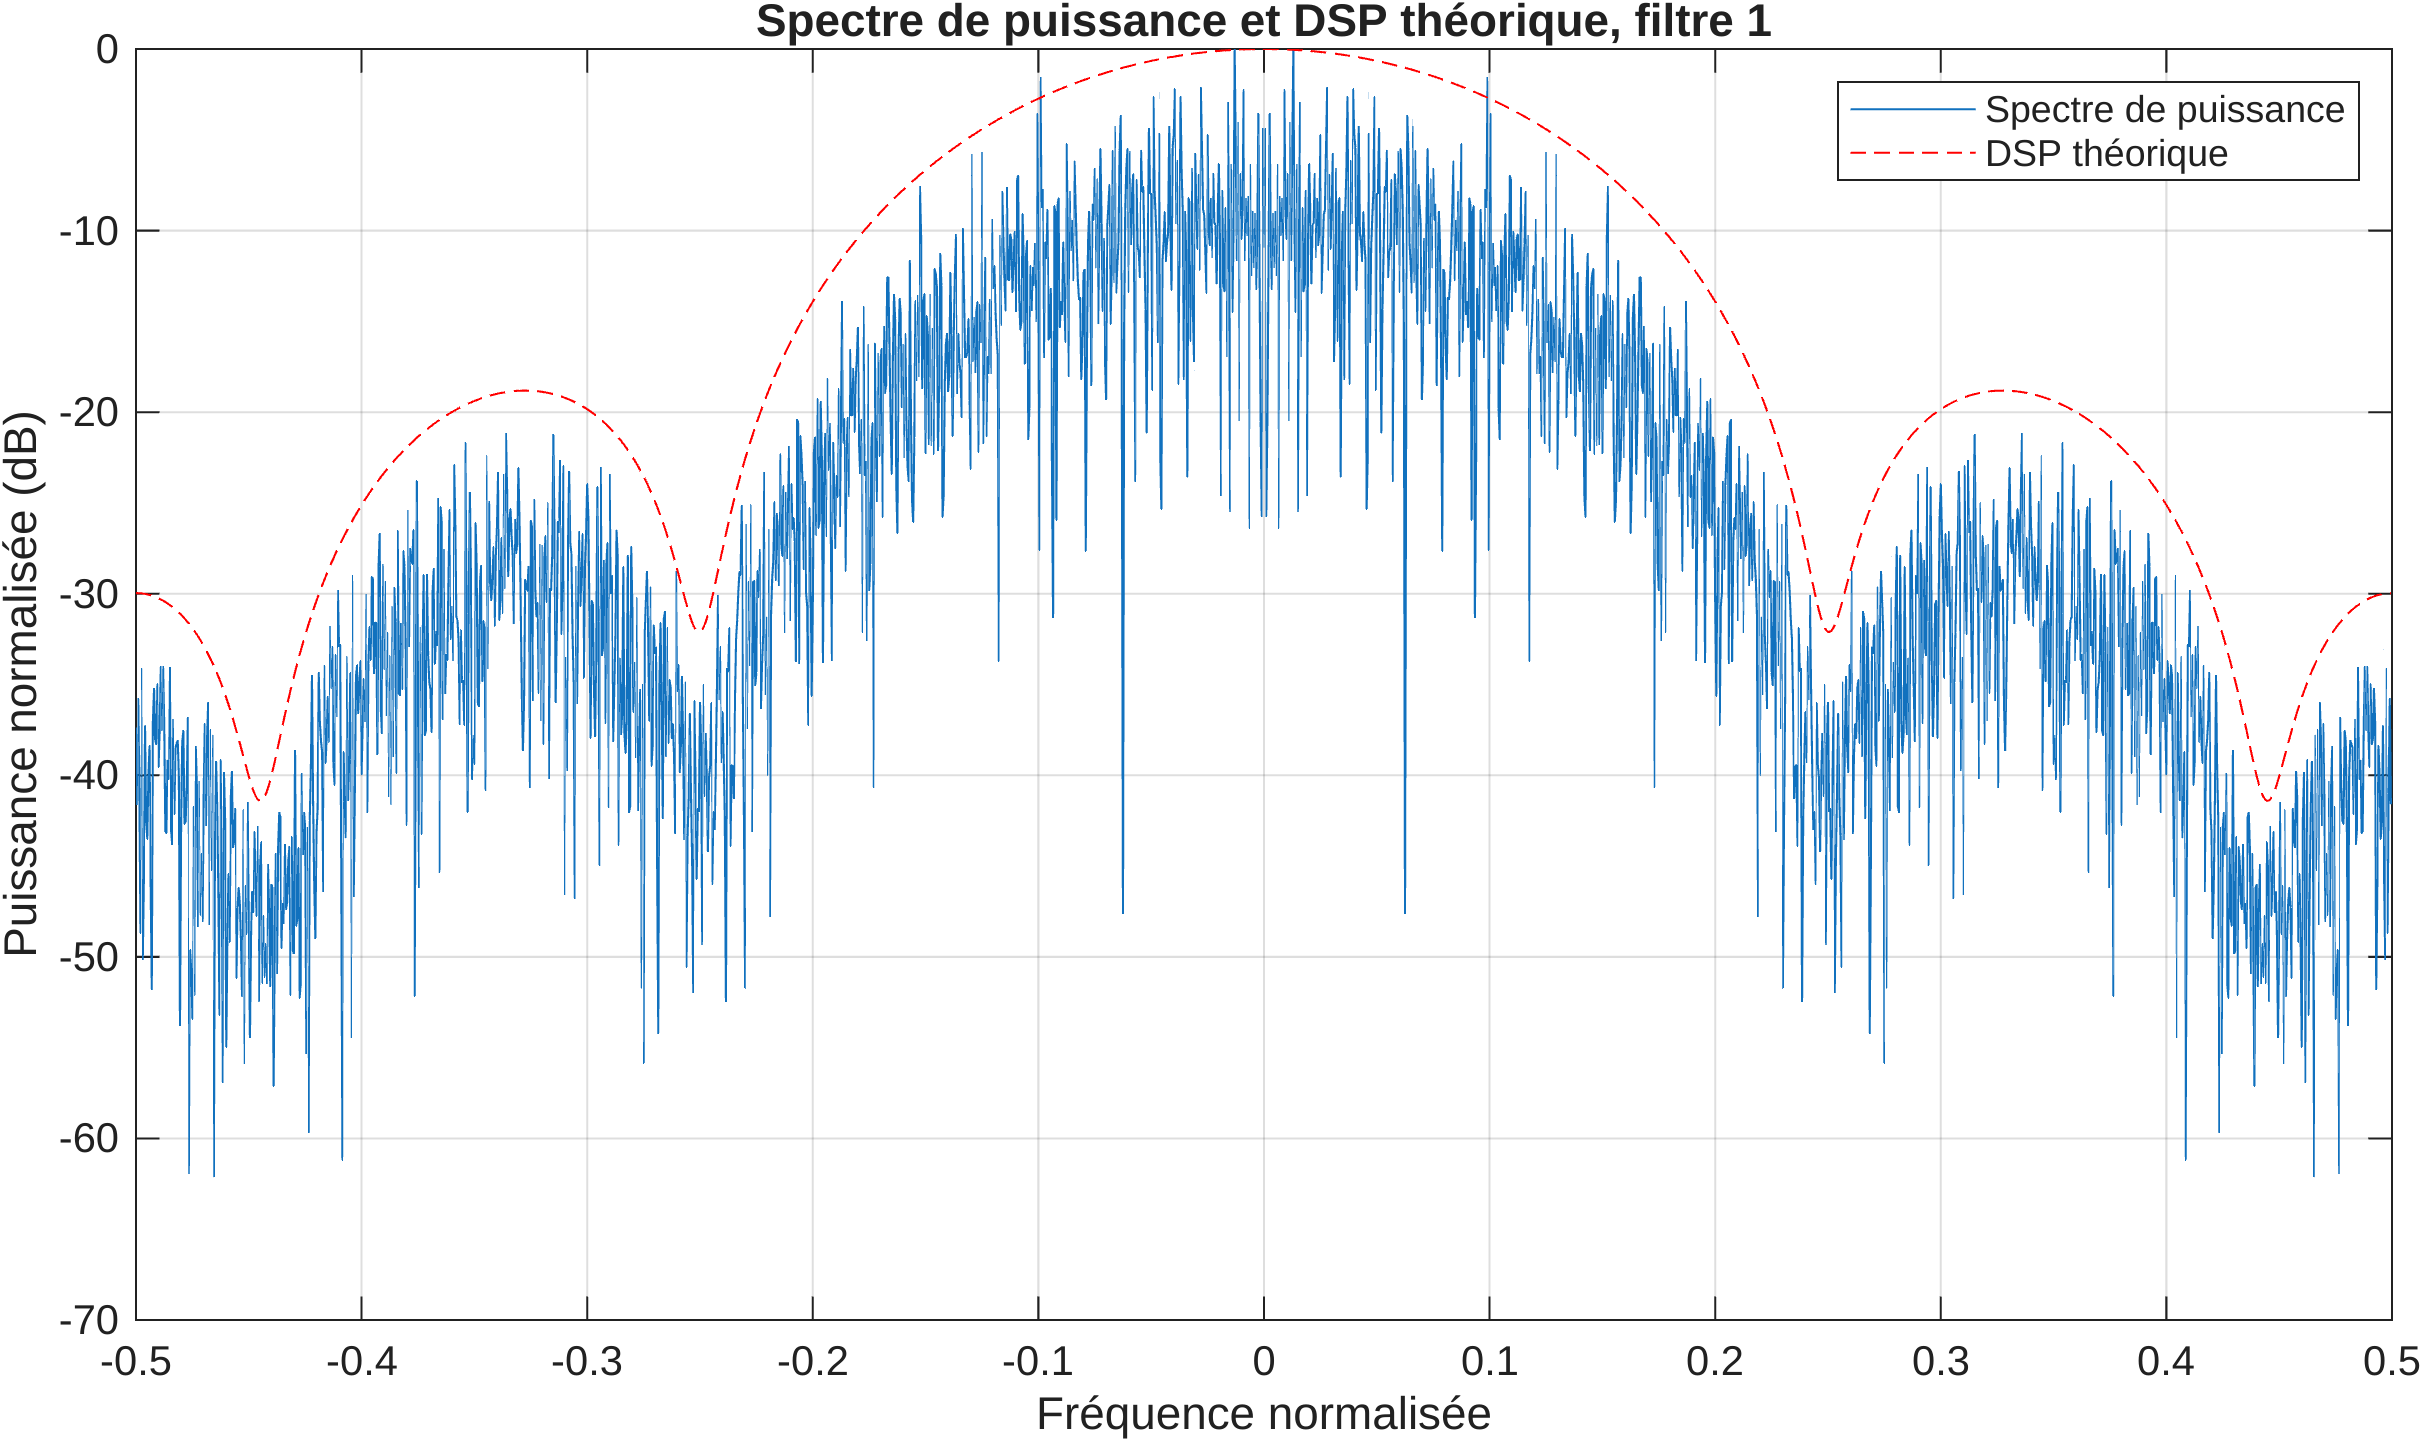
\includegraphics[width=\linewidth]{fig05.png}
    \caption{MA(4)}
  \end{subfigure}
  \begin{subfigure}{0.43\linewidth}
    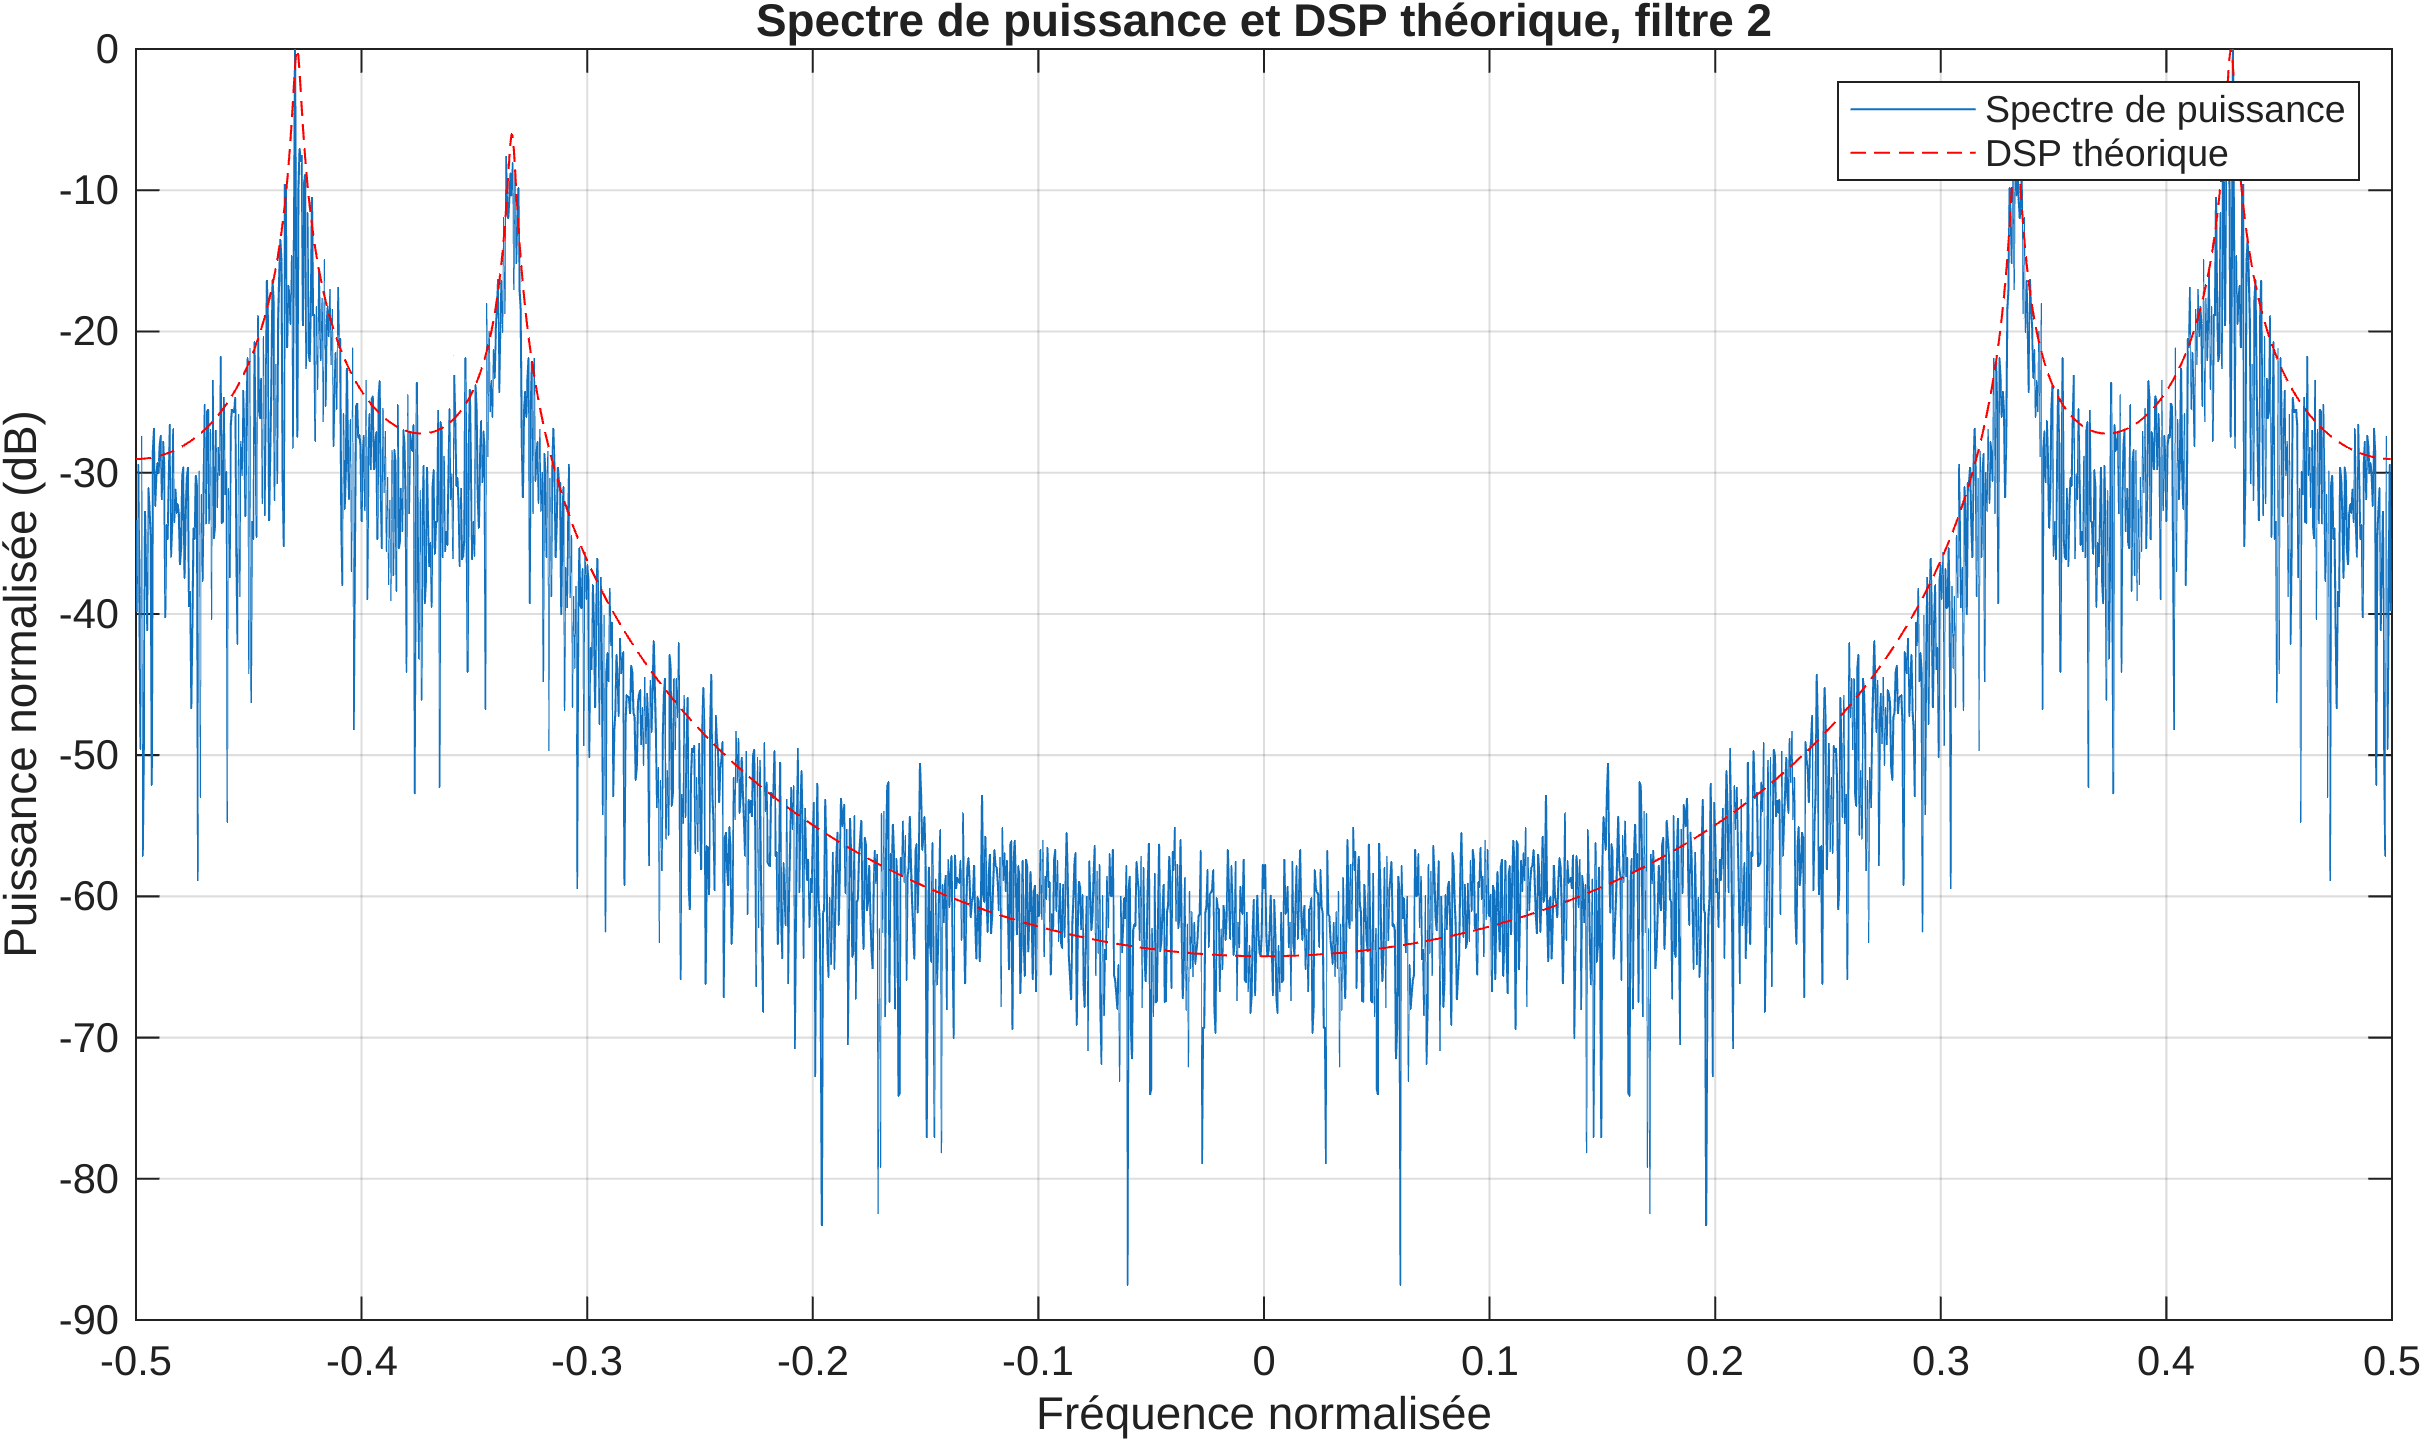
\includegraphics[width=\linewidth]{fig06.png}
    \caption{AR(4)}
  \end{subfigure}
  \caption{Spectre de puissance d'une réalisation (bleu) et DSP théorique (rouge), normalisés par leur maximum.}
  \label{fig:dsp_ma}
\end{figure}

\subsection{Estimation spectrale}

\subsubsection{Le périodogramme et ses limites}

Le spectre de puissance de la section précédente est le \emph{périodogramme} :
\begin{equation}
  I_N(\nu) = \frac{1}{N} \left| \sum_{n=0}^{N-1} x(n)\, e^{-j 2 \pi \nu n} \right|^2.
  \label{eq:perio}
\end{equation}
C'est un estimateur asymptotiquement sans biais de $S_x(\nu)$, mais il n'est pas consistant : sa variance $\operatorname{Var}[I_N(\nu)] \approx S_x^2(\nu)$ ne diminue pas quand $N$ augmente. Aux fréquences $\nu_k = k/N$, les valeurs de $I_N$ sont asymptotiquement indépendantes et suivent une loi exponentielle de moyenne $S_x(\nu_k)$. En décibels, cela se traduit par un écart-type d'environ $5{,}6$~dB, quel que soit $N$, ce qui correspond aux fluctuations observées sur la figure~\ref{fig:dsp_ma}.

Les estimateurs étudiés ci-après réduisent cette variance en moyennant, au prix d'une perte de résolution : c'est le compromis biais-variance. Pour fixer leurs paramètres, on compare leur résolution à la largeur à mi-hauteur $\Delta$ de la structure spectrale la plus étroite, soit $\Delta \approx (1-\rho)/(\pi\rho)$ pour une paire de zéros ou de pôles de module $\rho$ :
\begin{equation}
  \Delta_{MA} = \frac{1-R}{\pi R} \approx 0{,}0167,
  \qquad
  \Delta_{AR} = \frac{1-r}{\pi r} \approx 0{,}0032.
  \label{eq:fwhm}
\end{equation}
Les pics de l'AR(4) ne couvrent ainsi qu'environ six points fréquentiels de la grille $k/N$ : cette finesse conditionne tous les choix qui suivent.

\subsubsection{Périodogramme de Daniell}

Le périodogramme de Daniell lisse le périodogramme~\eqref{eq:perio} par une moyenne mobile de $2m+1$ points dans le domaine fréquentiel :
\begin{equation}
  \hat{S}_{D}(\nu_k) = \frac{1}{2m + 1} \sum_{j = -m}^{m} I_N(\nu_{k + j}),
  \qquad
  \operatorname{Var}\big[\hat{S}_{D}\big] \approx \frac{S_x^2}{2m+1}.
  \label{eq:daniell}
\end{equation}
Pour réduire la variance autant que possible sans déformer le spectre, la largeur de la fenêtre de lissage doit rester inférieure à la largeur à mi-hauteur : $(2m+1)/N < \Delta$. Ce critère est approché, mais il donne un ordre de grandeur pertinent. Avec~\eqref{eq:fwhm}, il impose $2m+1 < 33{,}5$ pour le MA(4) et $2m+1 < 6{,}4$ pour l'AR(4). On choisit donc $m_{MA} = 16$ et $m_{AR} = 2$.

Ce calcul met en évidence la limite du périodogramme de Daniell (figure~\ref{fig:daniell}) :
\begin{itemize}
  \item pour le MA(4), dont la DSP varie lentement, la fenêtre admissible permet un lissage efficace : la variance est divisée par 33 et l'estimée suit fidèlement la DSP. Les creux sont toutefois légèrement comblés ($-39$~dB au lieu de $-41$~dB en $\nu = 4/9$), car la fenêtre de lissage a la même largeur que le creux ;
  \item pour l'AR(4), le critère limite la fenêtre à 5 points : les pics sont bien localisés, mais la variance n'est divisée que par 5 et le tracé reste bruité. Le niveau autour de $\nu = 0$ est en outre surestimé d'environ $9$~dB, sous l'effet combiné de la normalisation par le maximum (le lissage abaisse le sommet des pics) et de la fuite spectrale de la fenêtre rectangulaire implicite, sensible sur 64~dB de dynamique.
\end{itemize}
On ne peut donc pas lisser efficacement un spectre très résonant sans en écrêter les extrema.

\begin{figure}[!htb]
  \centering
  \begin{subfigure}{0.43\linewidth}
    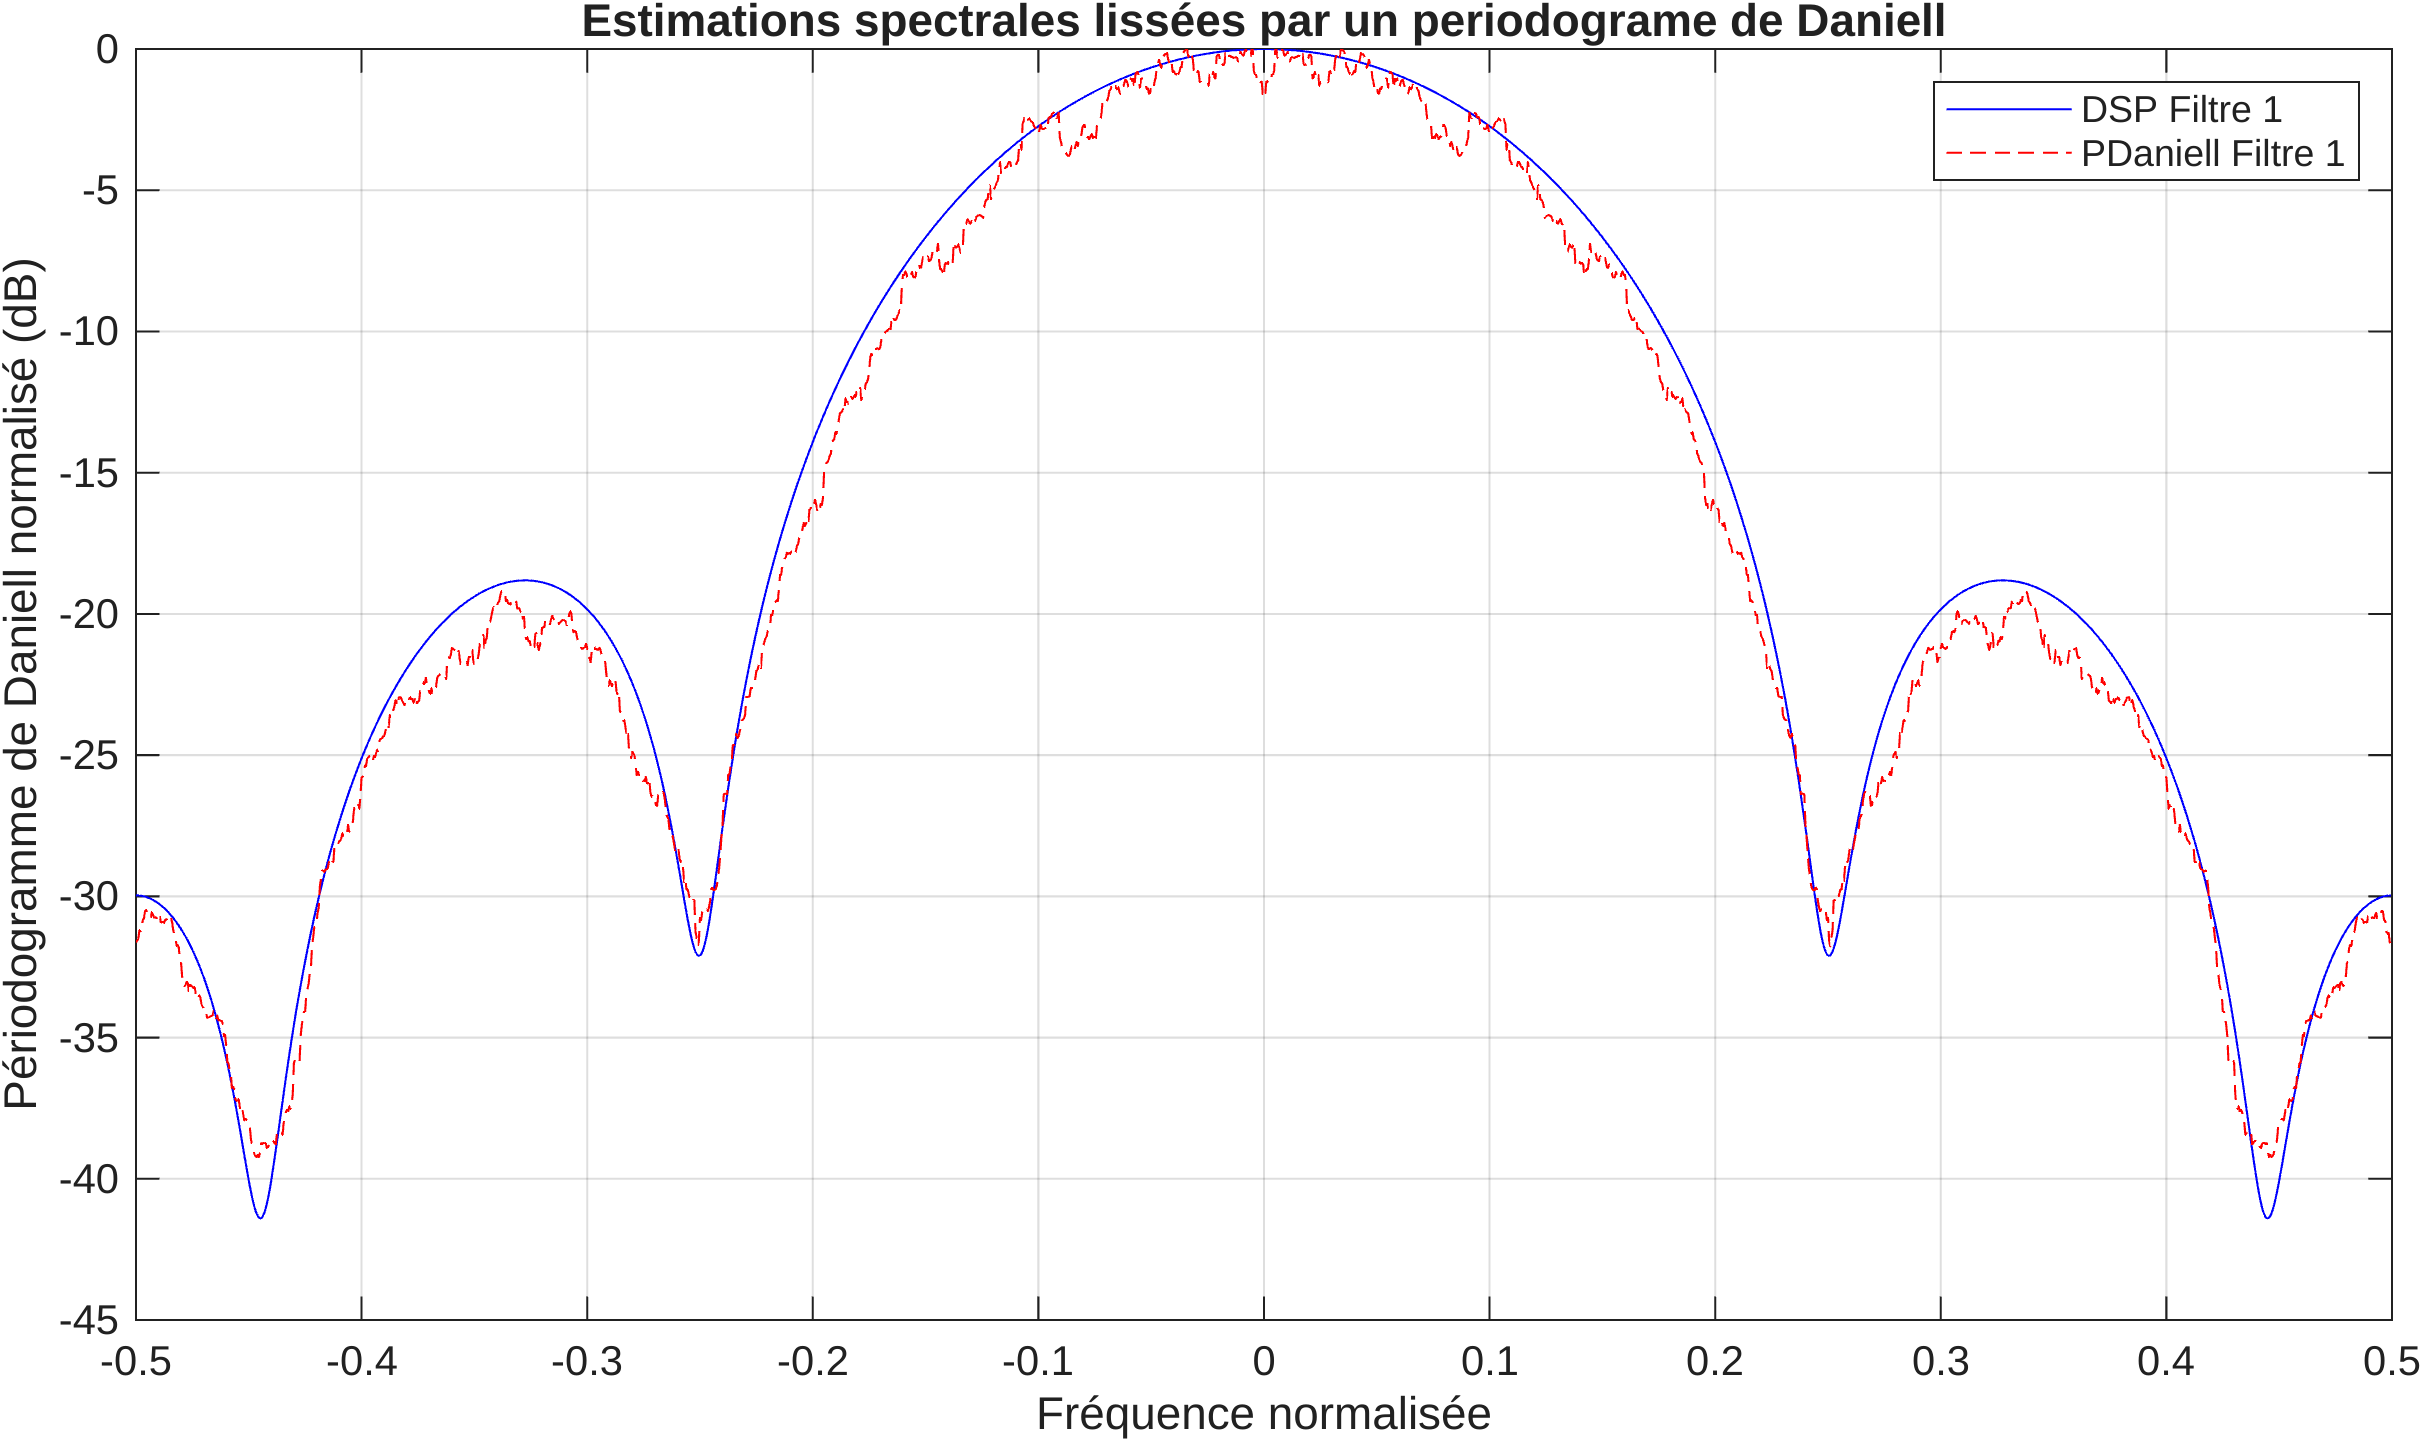
\includegraphics[width=\linewidth]{fig07.png}
    \caption{MA(4), $2m+1 = 33$}
  \end{subfigure}
  \begin{subfigure}{0.43\linewidth}
    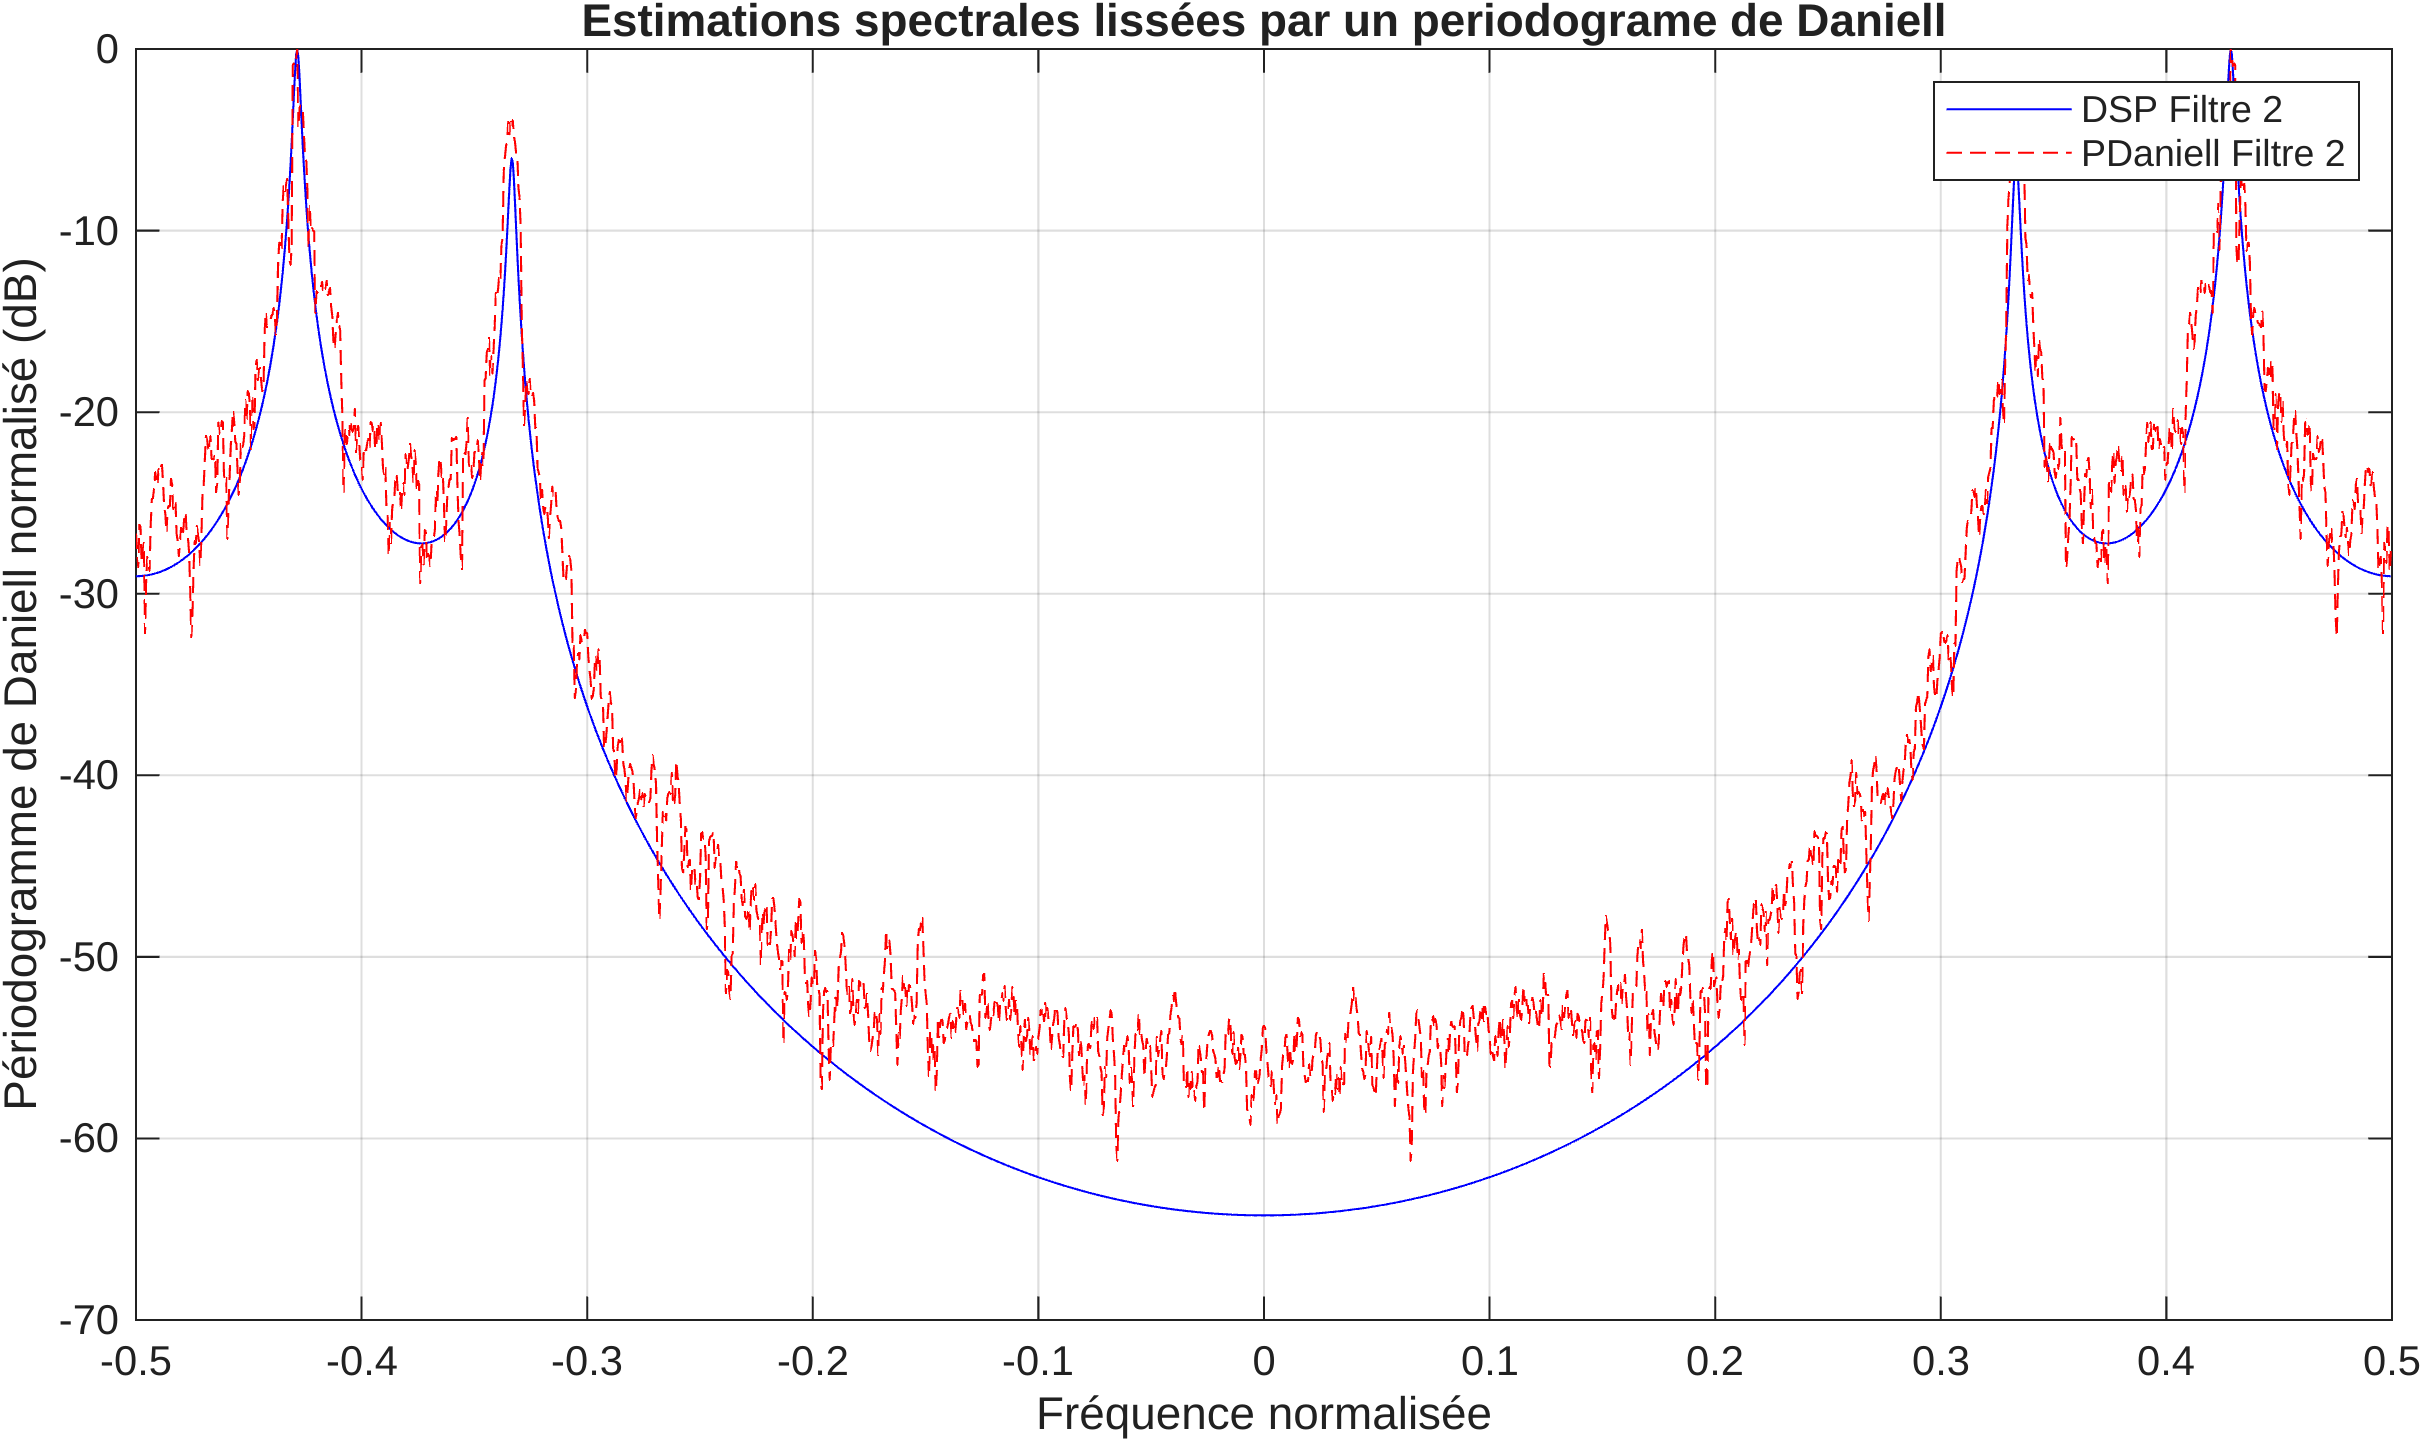
\includegraphics[width=\linewidth]{fig08.png}
    \caption{AR(4), $2m+1 = 5$}
  \end{subfigure}
  \caption{Périodogrammes de Daniell (rouge) comparés à la DSP théorique (bleu).}
  \label{fig:daniell}
\end{figure}

\subsubsection{Périodogramme de Bartlett}

Le périodogramme de Bartlett~[2] découpe le signal en $K$ blocs disjoints de longueur $L$, avec $K = N/L$, calcule le périodogramme~\eqref{eq:perio} sur chaque bloc puis en fait la moyenne arithmétique :
\begin{equation}
  I_i(\nu) = \frac{1}{L} \left| \sum_{n=0}^{L-1} x_i(n)\, e^{-j 2 \pi \nu n} \right|^2,
  \qquad
  \hat{S}_{B}(\nu) = \frac{1}{K} \sum_{i=1}^{K} I_i(\nu),
  \qquad
  \operatorname{Var}\big[\hat{S}_{B}\big] \approx \frac{S_x^2}{K}.
  \label{eq:bartlett}
\end{equation}
La résolution n'est plus $1/N$ mais environ $1/L$. La condition de non-distorsion devient $1/L < \Delta$, soit $L > 1/\Delta$ : $L_{MA} \geq 60$ et $L_{AR} \geq 313$. On retient $L_{MA} = 80$ ($K = 25$) et $L_{AR} = 400$ ($K = 5$). Pour l'AR(4), on retrouve le facteur de réduction de variance de 5 obtenu avec Daniell : la contrainte de résolution limite de la même façon le nombre de moyennes.

Le périodogramme de Bartlett présente en outre deux défauts (figure~\ref{fig:bartlett}) :
\begin{itemize}
  \item une \emph{fuite spectrale} importante : le découpage revient à pondérer chaque bloc par une fenêtre rectangulaire, donc à convoluer le spectre par un noyau de type sinus cardinal, dont les lobes secondaires culminent à $-13$~dB. Sur le MA(4), les creux sont comblés ($-25$~dB au lieu de $-32$~dB en $1/4$, $-30$~dB au lieu de $-41$~dB en $4/9$) ; sur l'AR(4), le plancher remonte de $-64$~dB à $-43$~dB. Le critère de résolution, qui ne porte que sur le lobe principal, est donc nécessaire mais pas suffisant lorsque la dynamique est grande ;
  \item un nombre de moyennes limité par le découpage en blocs disjoints, alors qu'un recouvrement permettrait d'augmenter $K$ sans réduire $L$.
\end{itemize}

\begin{figure}[!htb]
  \centering
  \begin{subfigure}{0.43\linewidth}
    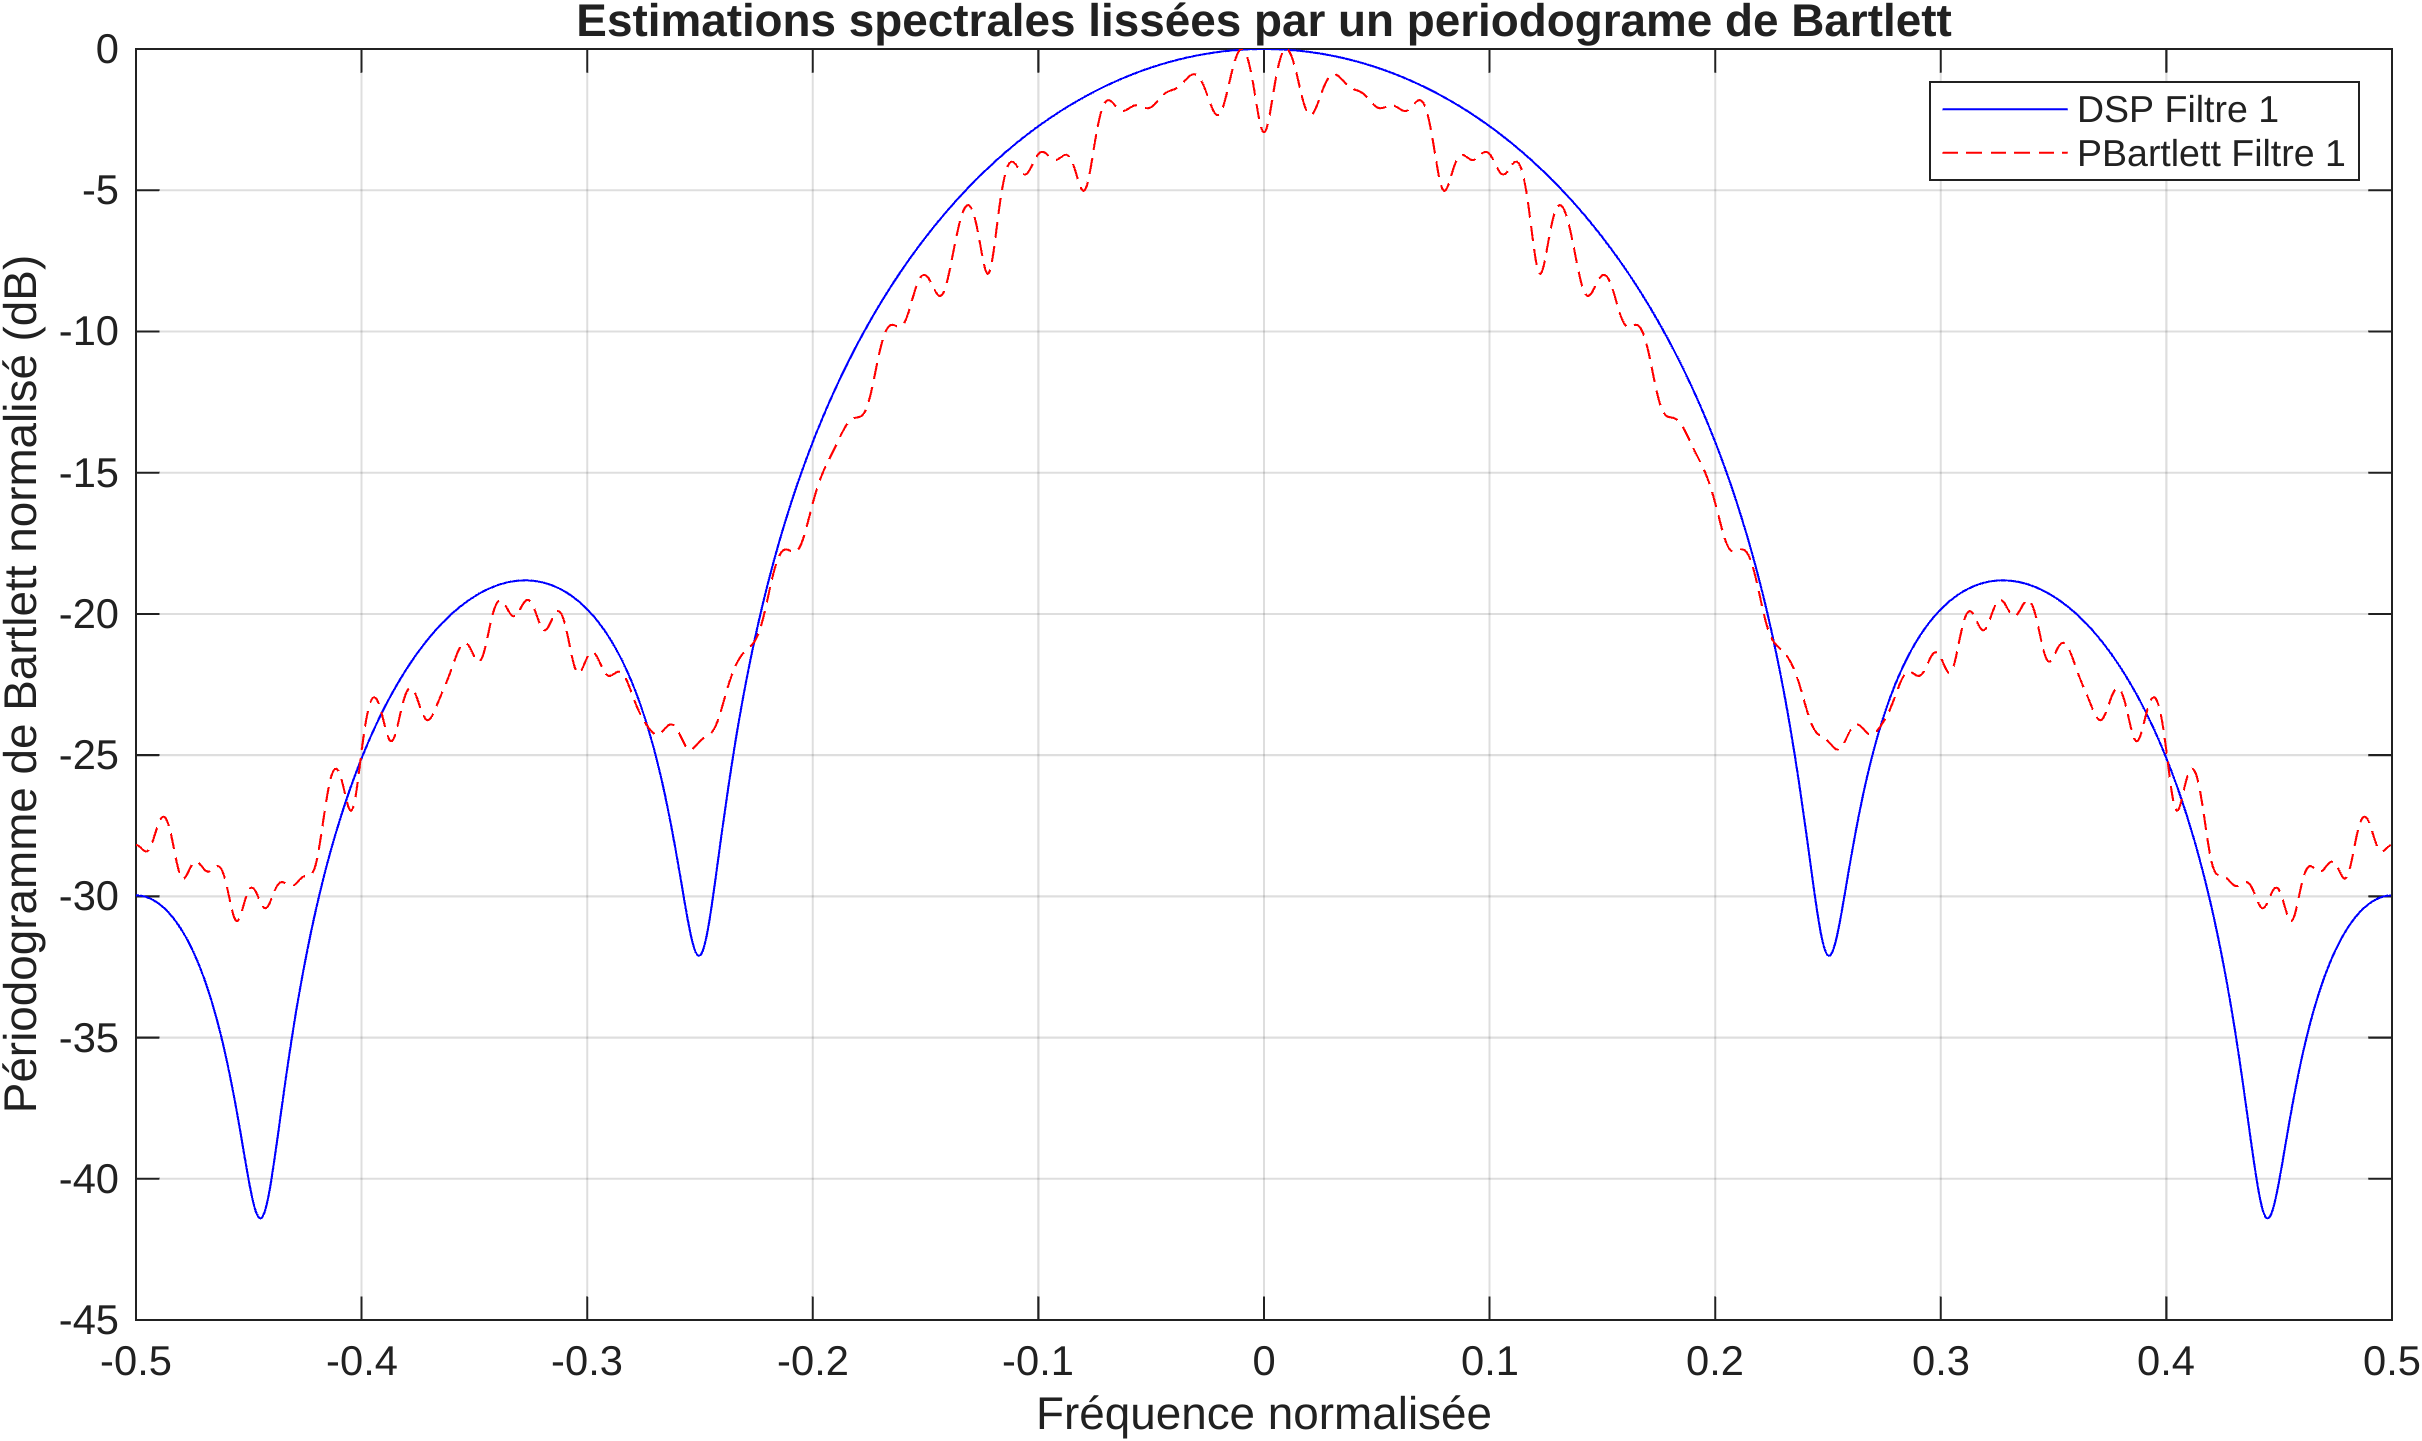
\includegraphics[width=\linewidth]{fig09.png}
    \caption{MA(4), $L = 80$, $K = 25$}
  \end{subfigure}
  \begin{subfigure}{0.43\linewidth}
    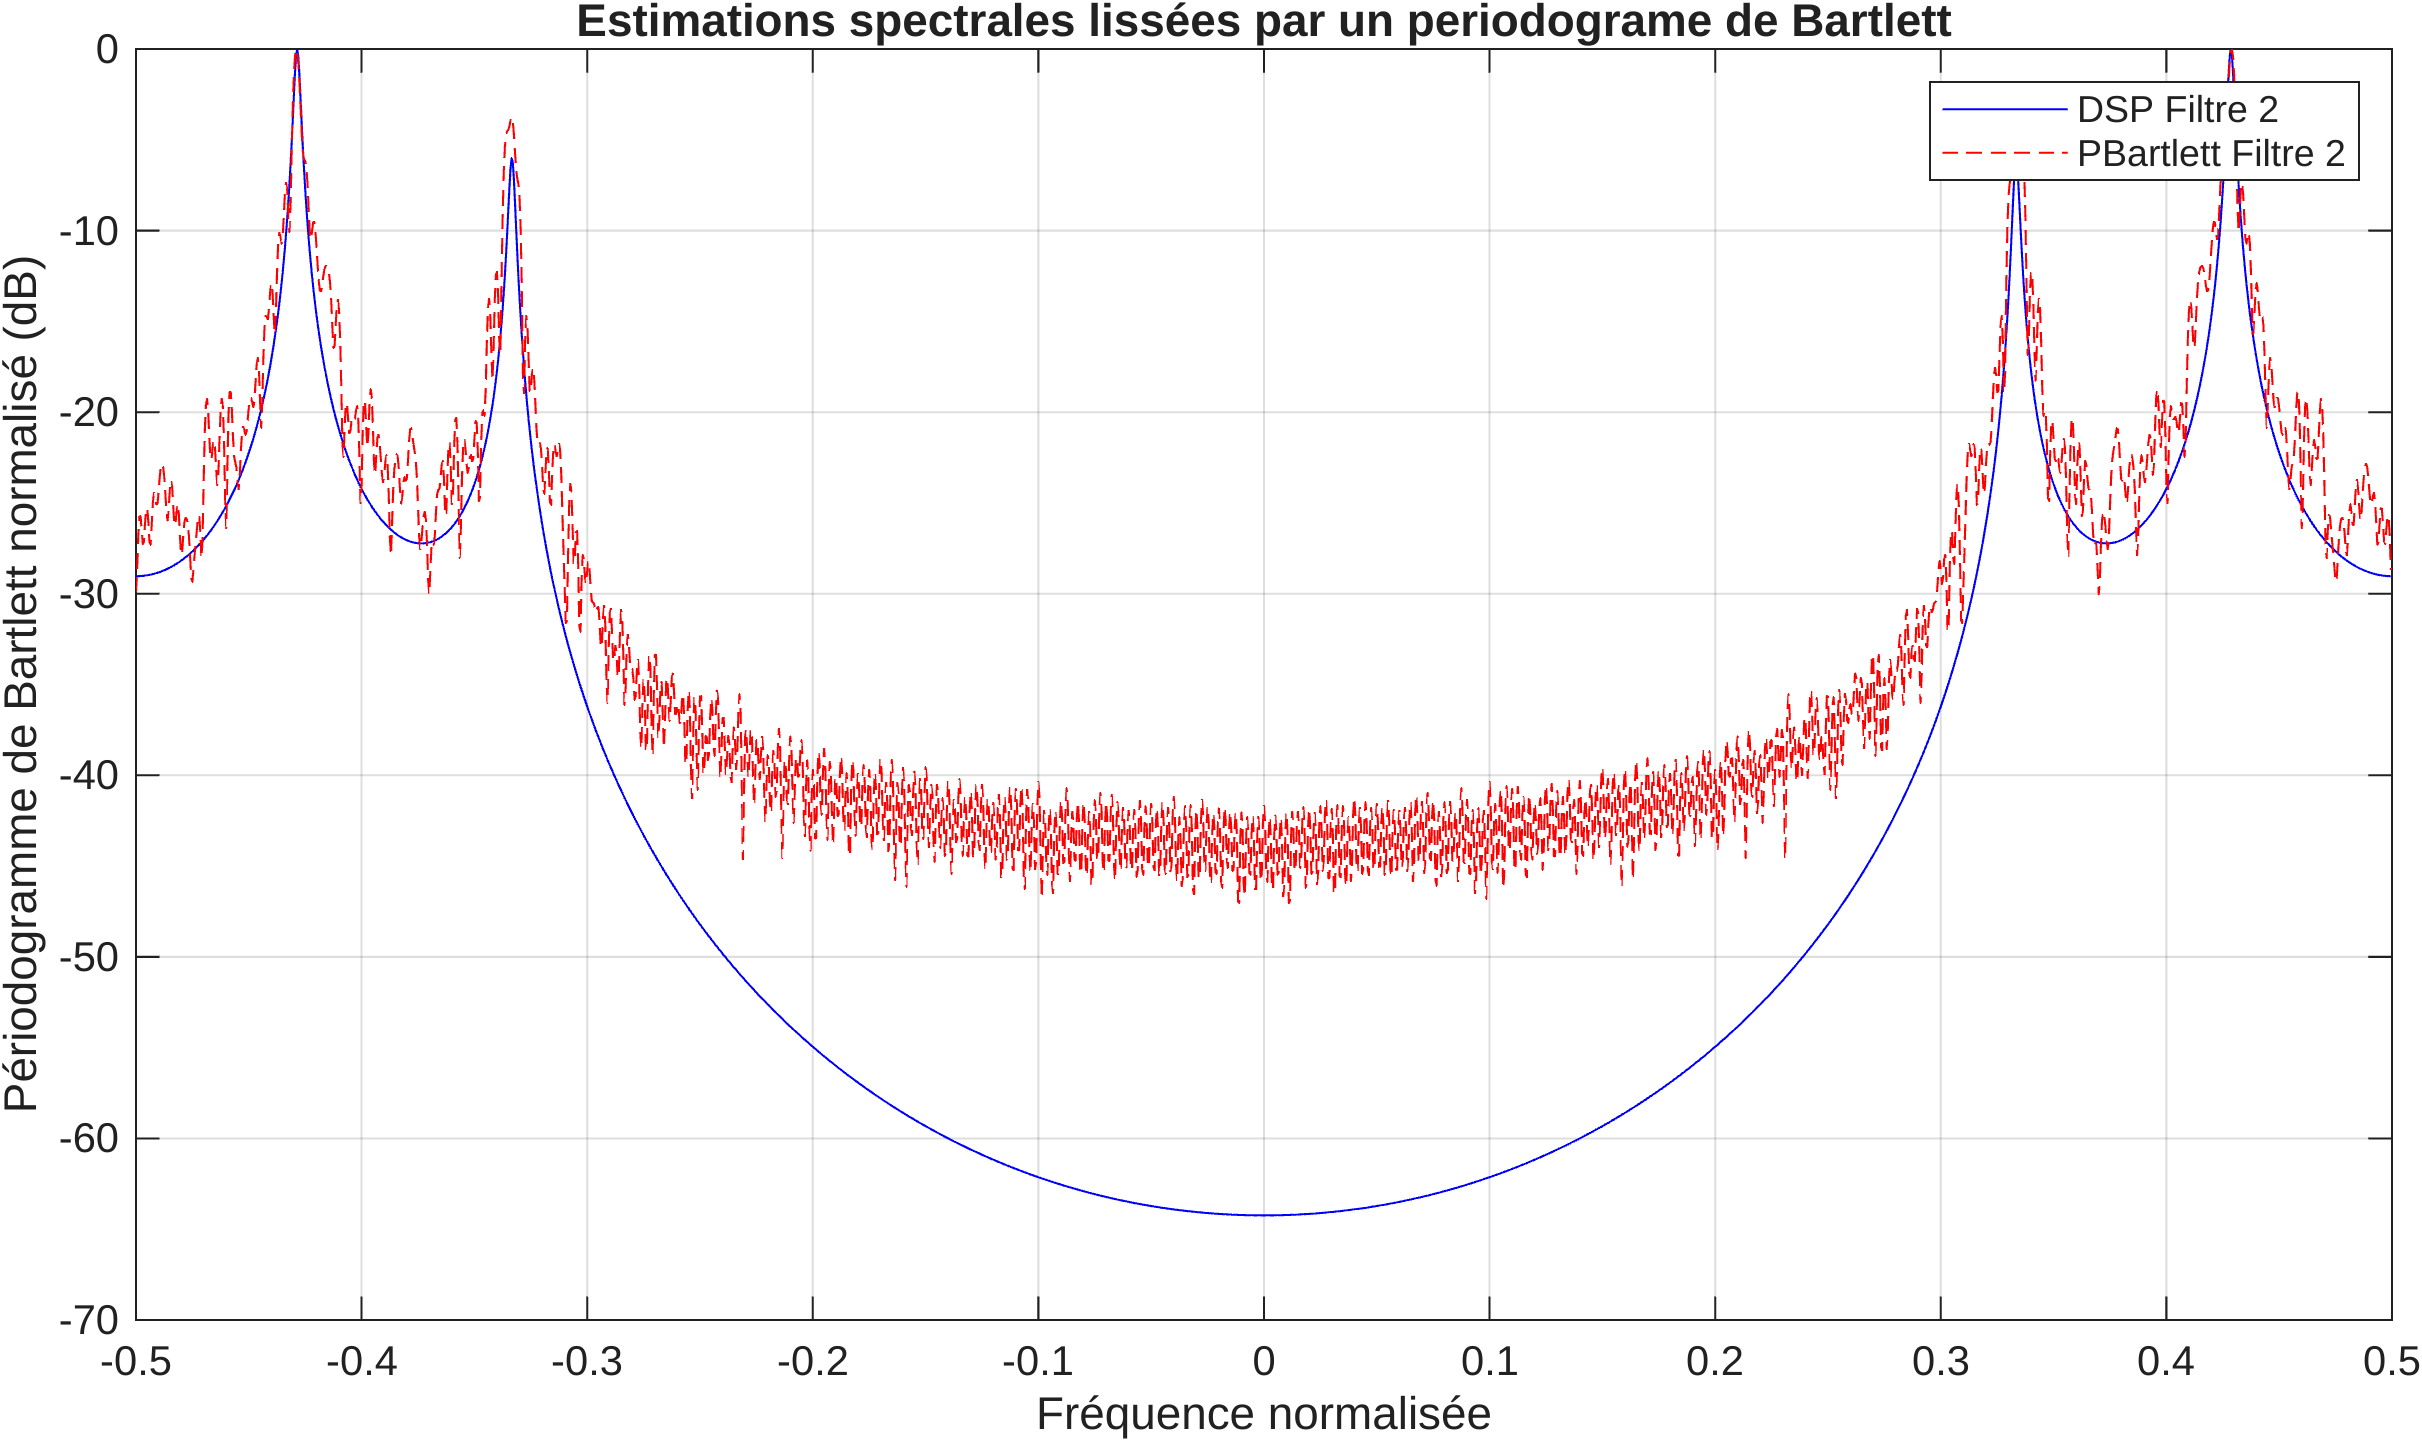
\includegraphics[width=\linewidth]{fig10.png}
    \caption{AR(4), $L = 400$, $K = 5$}
  \end{subfigure}
  \caption{Périodogrammes de Bartlett (rouge) comparés à la DSP théorique (bleu).}
  \label{fig:bartlett}
\end{figure}

\subsubsection{Périodogramme de Welch}

Le périodogramme de Welch~[1] reprend le principe de Bartlett et corrige ses deux défauts. Chaque segment est pondéré par une fenêtre non rectangulaire $w(n)$, ici la fenêtre de Hann, et deux segments successifs se recouvrent. Avec un décalage $D$ entre segments :
\begin{equation}
  I_i(\nu) = \frac{1}{L\, U} \left| \sum_{n=0}^{L-1} w(n)\, x\big(n + (i-1)D\big)\, e^{-j 2 \pi \nu n} \right|^2,
  \qquad
  U = \frac{1}{L} \sum_{n=0}^{L-1} w^2(n),
  \qquad
  \hat{S}_{W}(\nu) = \frac{1}{K} \sum_{i=1}^{K} I_i(\nu).
  \label{eq:welch}
\end{equation}
Le facteur $U$ compense la perte d'énergie due à la fenêtre et rend l'estimateur asymptotiquement sans biais. La fenêtre de Hann abaisse le premier lobe secondaire à $-31$~dB, avec une décroissance de 18~dB par octave contre 6 pour la fenêtre rectangulaire~[4]. En contrepartie, son lobe principal est deux fois plus large : la résolution passe d'environ $1/L$ à $1{,}5/L$. Le critère devient $L > 1{,}5/\Delta$, d'où $L_{MA} = 100$ et $L_{AR} = 500$. Avec un recouvrement de 50~\% ($D = L/2$), $K = 2N/L - 1$, soit 39 et 7 segments. Les segments n'étant plus indépendants, la réduction de variance est un peu inférieure à $K$ : pour la fenêtre de Hann à 50~\%, $\operatorname{Var}[\hat{S}_W] \approx S_x^2/37$ pour le MA(4) et $S_x^2/6{,}7$ pour l'AR(4)~[1].

La figure~\ref{fig:welch} montre le meilleur compromis obtenu. Pour le MA(4), les deux creux sont restitués à leur profondeur exacte. Pour l'AR(4), le plancher remonte seulement à $-60$~dB environ. La comparaison avec Bartlett isole l'effet de la fenêtre : à longueurs de segment voisines (400 et 500), le plancher gagne près de 17~dB.

\begin{figure}[!htb]
  \centering
  \begin{subfigure}{0.43\linewidth}
    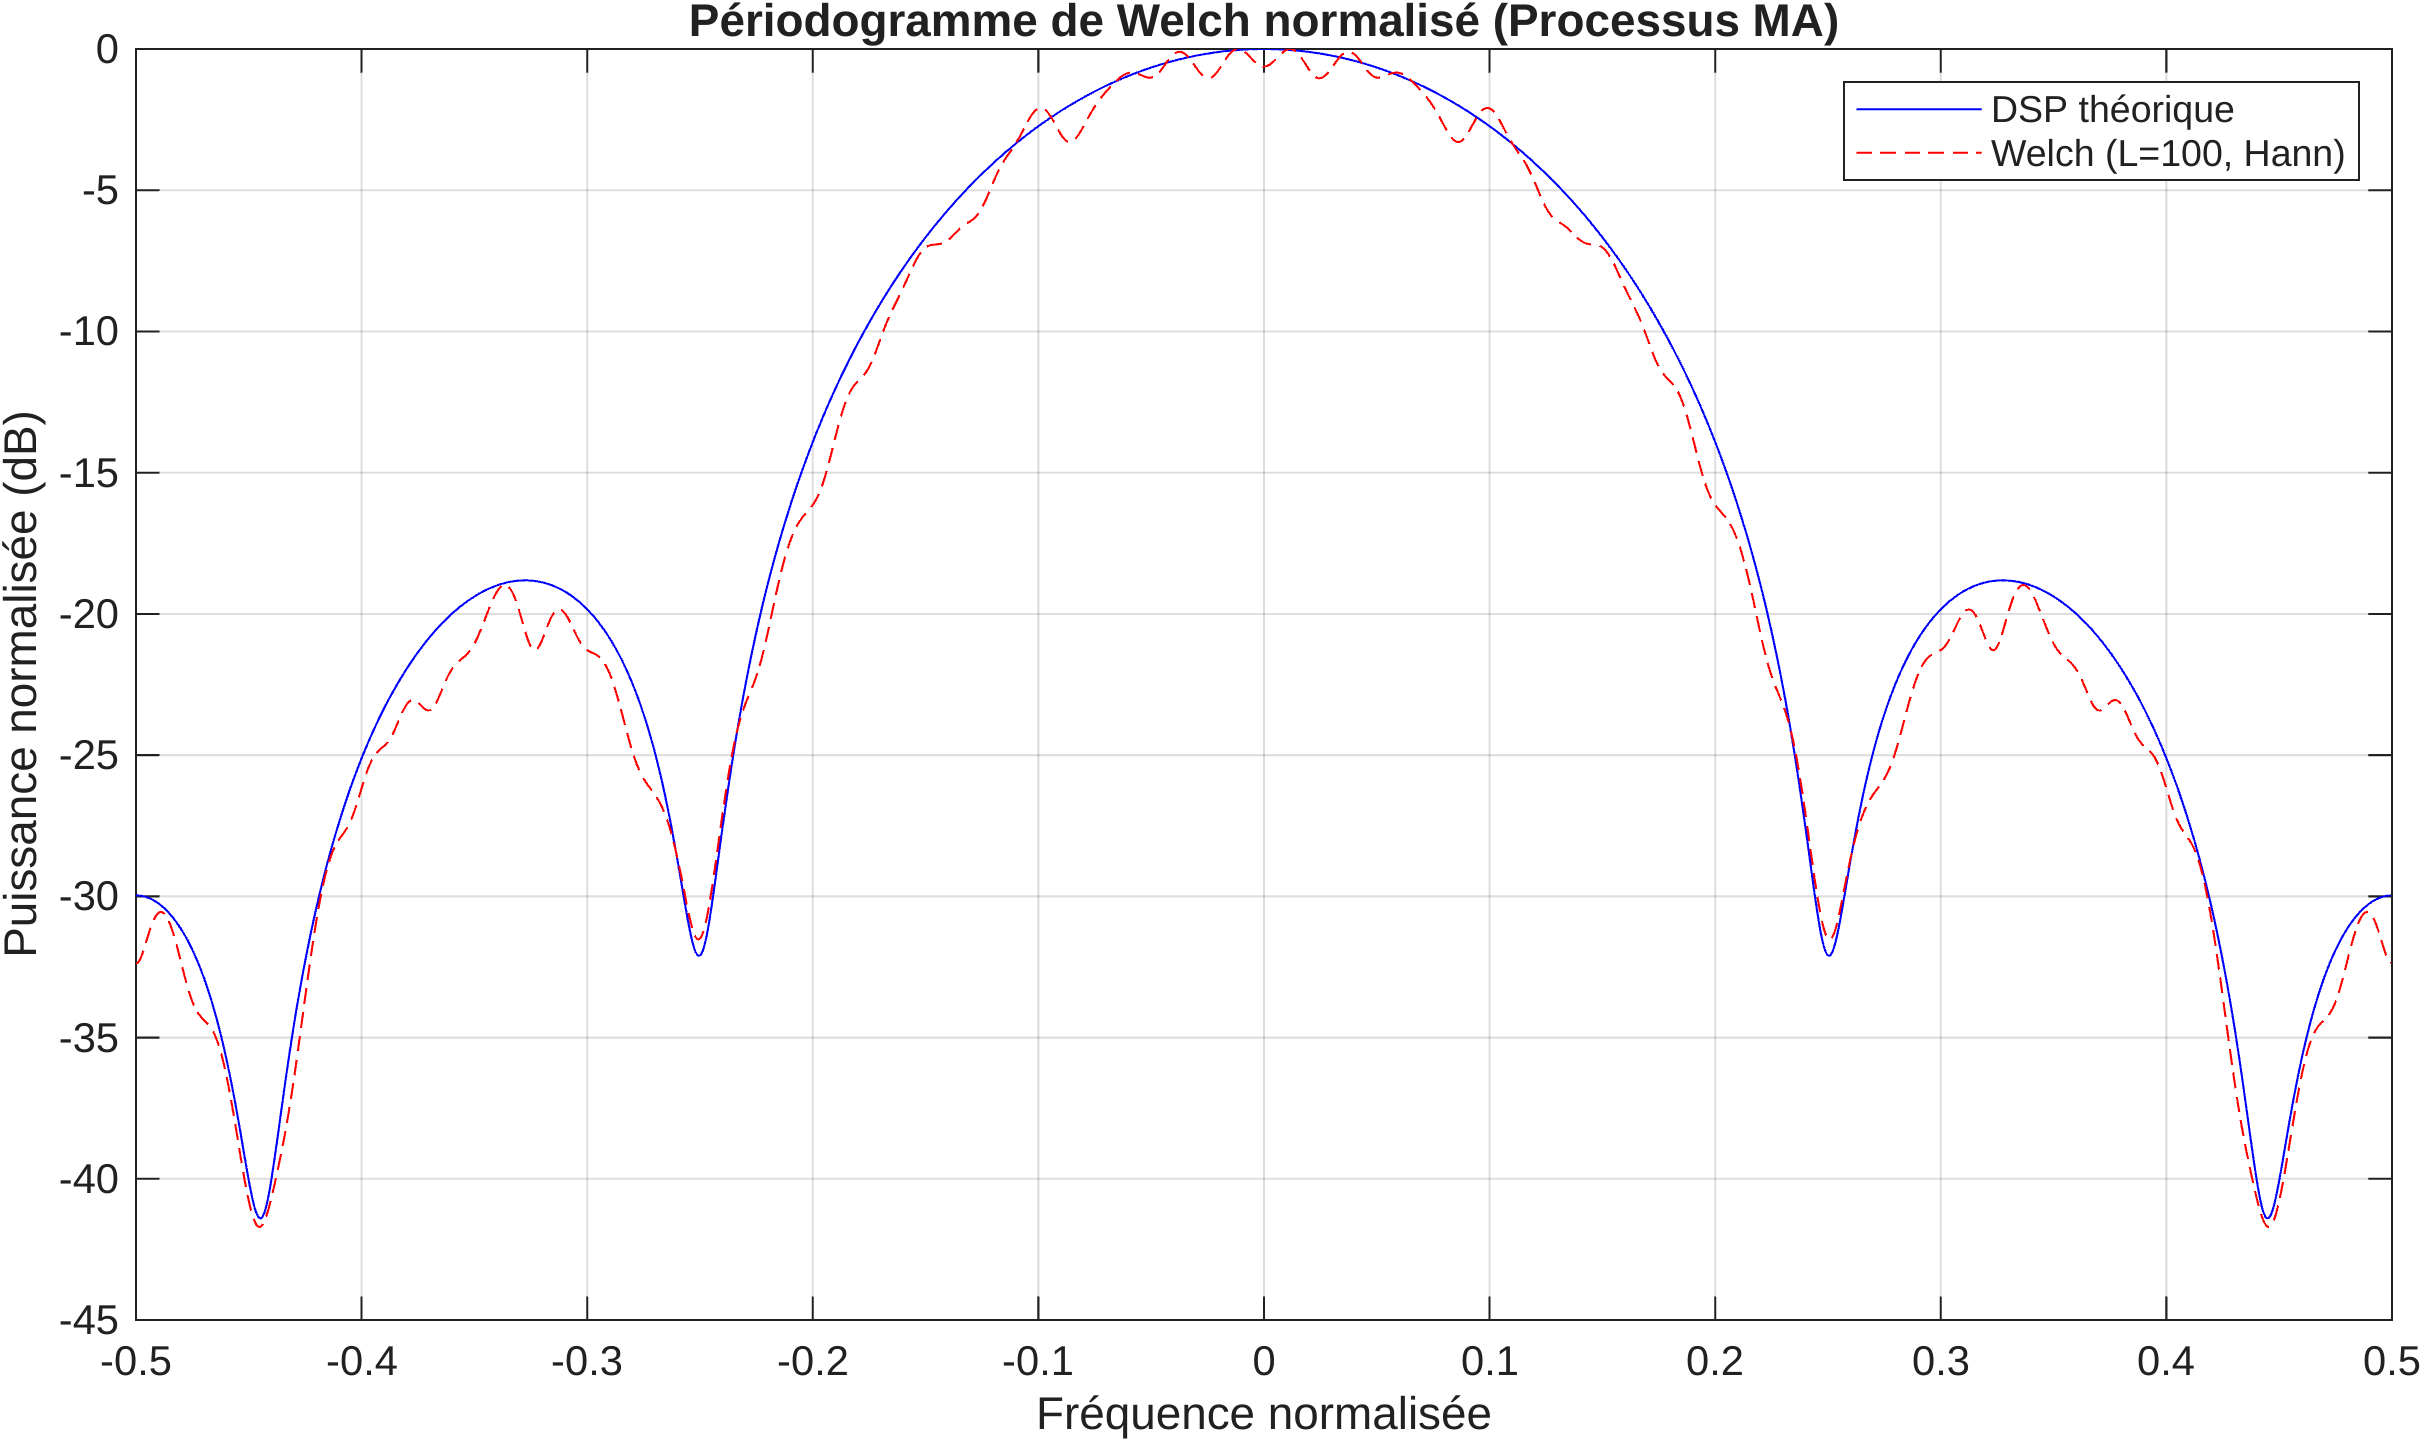
\includegraphics[width=\linewidth]{fig11.png}
    \caption{MA(4), $L = 100$, $K = 39$}
  \end{subfigure}
  \begin{subfigure}{0.43\linewidth}
    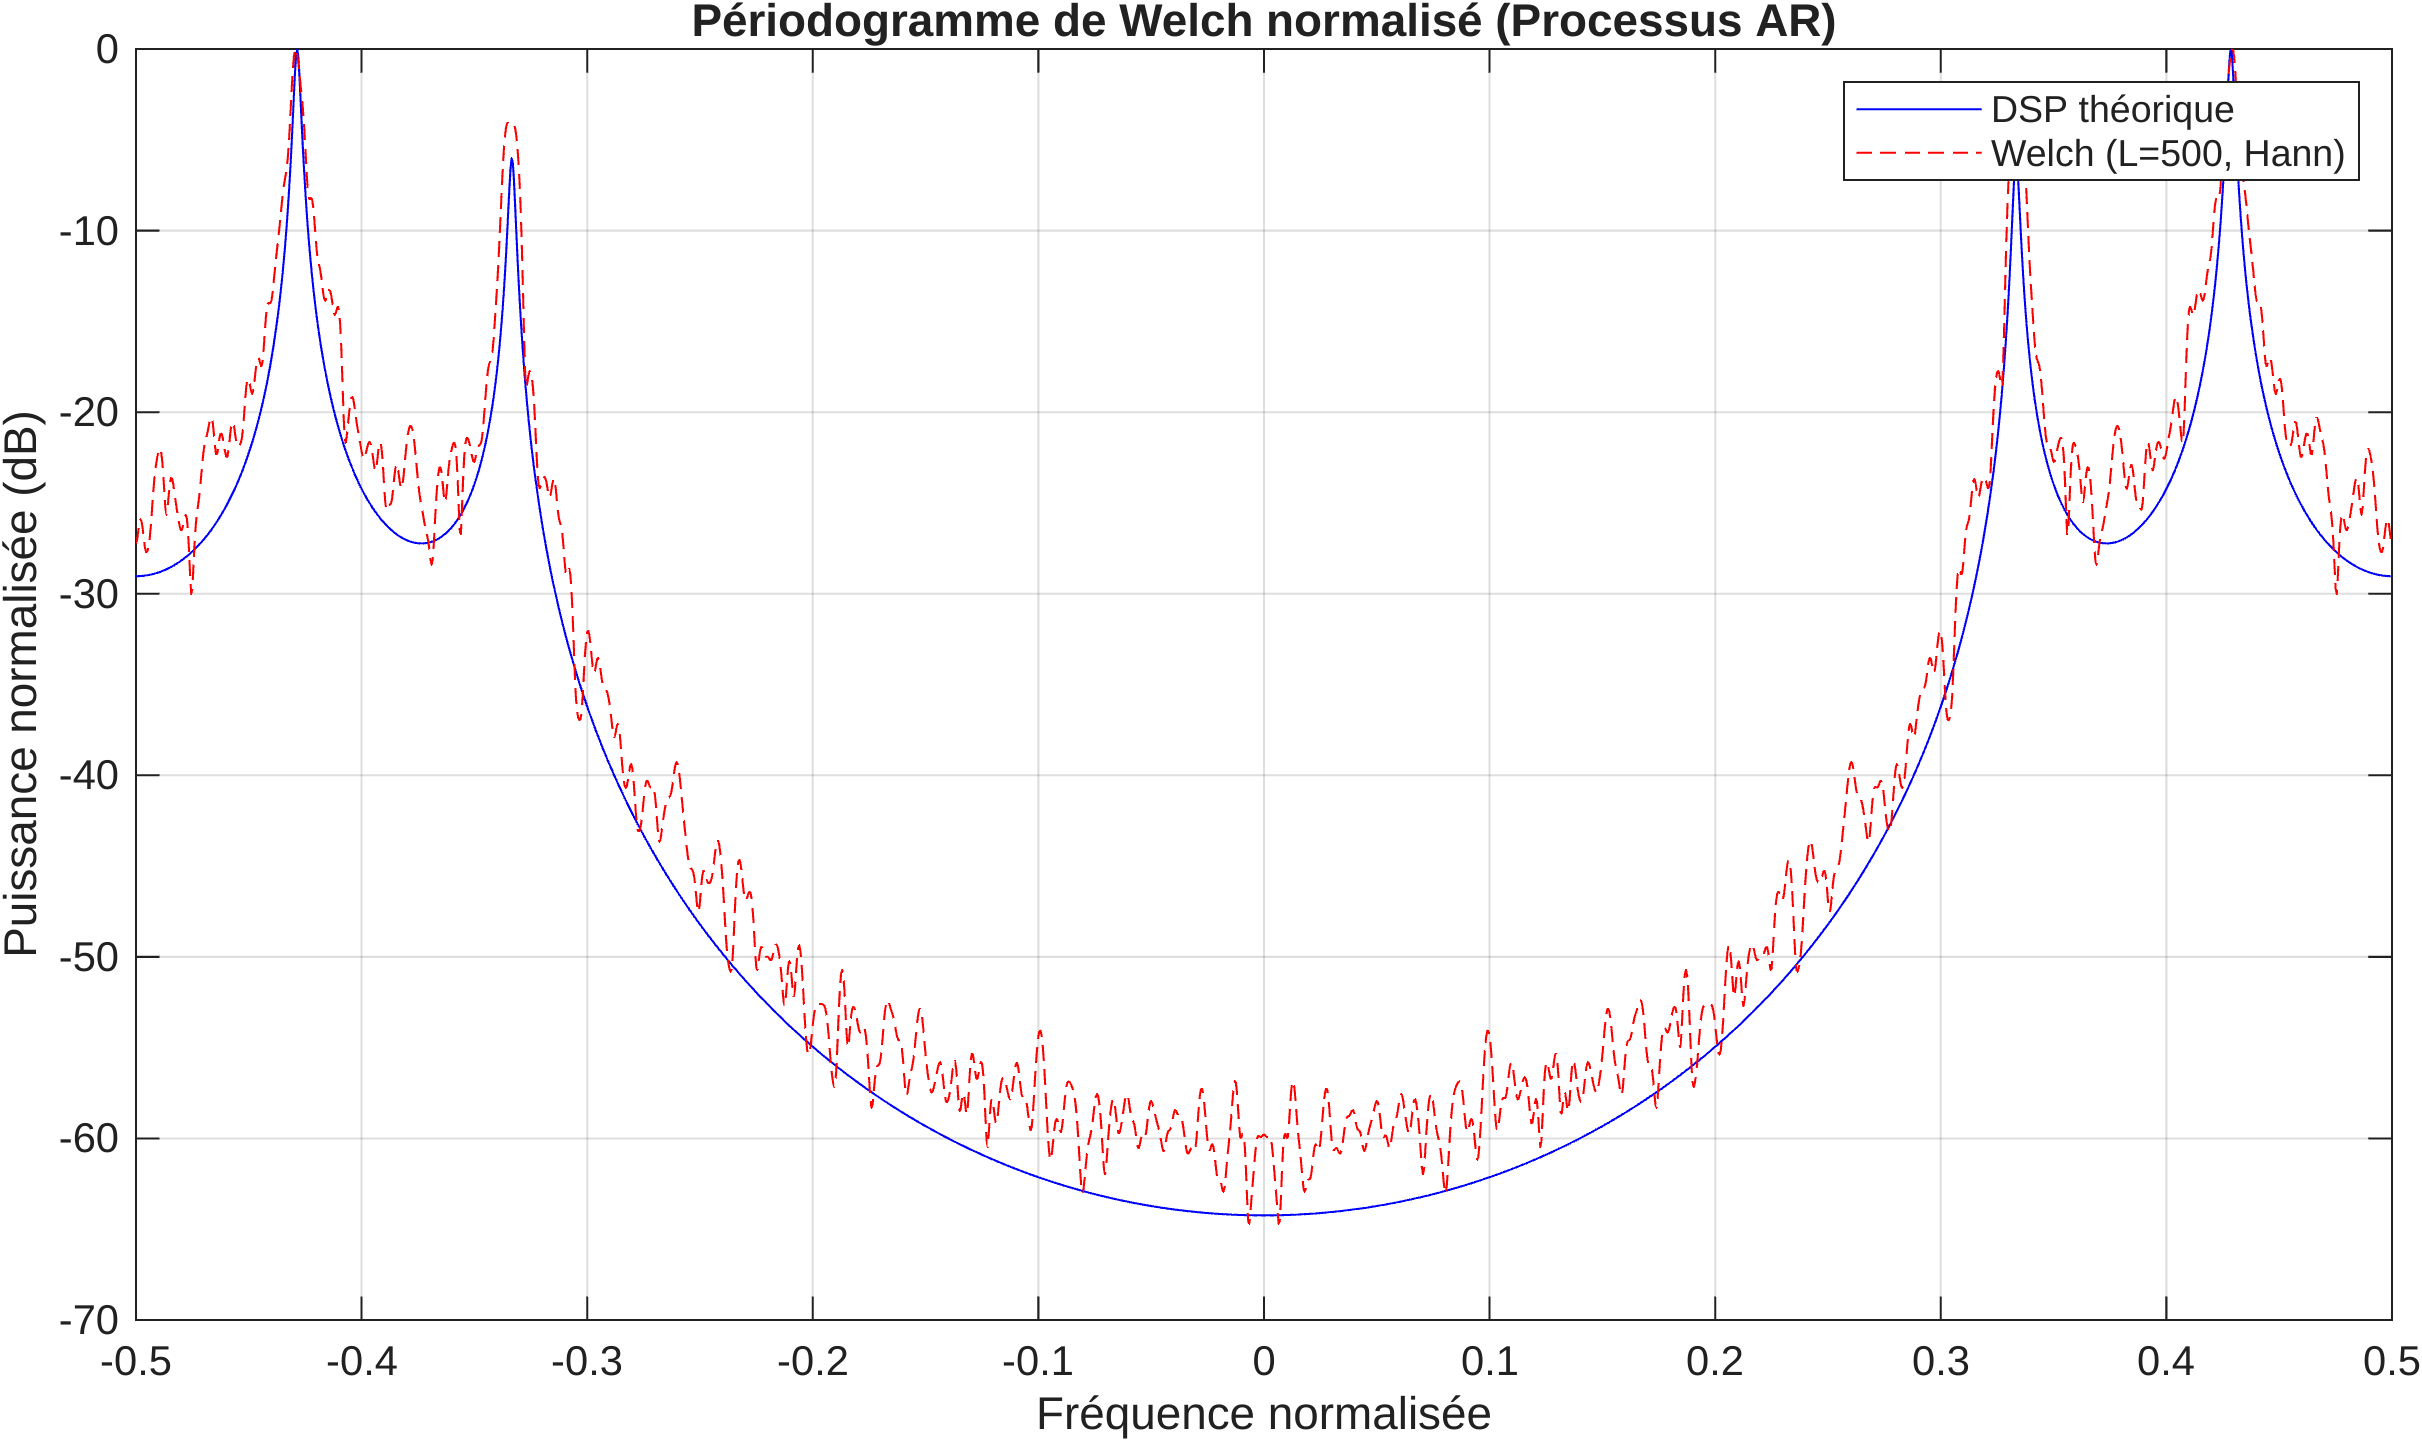
\includegraphics[width=\linewidth]{fig12.png}
    \caption{AR(4), $L = 500$, $K = 7$}
  \end{subfigure}
  \caption{Périodogrammes de Welch (Hann, recouvrement de 50~\%) comparés à la DSP théorique.}
  \label{fig:welch}
\end{figure}

\subsubsection{Corrélogramme}

Le corrélogramme, ou méthode de Blackman-Tukey~[3], s'appuie sur le théorème de Wiener-Khintchine : la DSP est la transformée de Fourier de l'autocorrélation. On estime donc l'autocorrélation, de manière biaisée, puis on en prend la transformée de Fourier après pondération par une fenêtre $w(k)$ de demi-longueur $K_{\max}$ :
\begin{equation}
  \hat{r}_x(k) = \frac{1}{N} \sum_{n=0}^{N-1-|k|} x(n)\, x(n+|k|),
  \qquad
  \hat{S}_{BT}(\nu) = \sum_{k=-K_{\max}}^{K_{\max}} w(k)\, \hat{r}_x(k)\, e^{-j2\pi\nu k}.
  \label{eq:bt}
\end{equation}
Sans troncature ni pondération ($K_{\max} = N-1$, $w = 1$), $\hat{S}_{BT}$ est \emph{exactement} égal au périodogramme~\eqref{eq:perio} : toute la réduction de variance provient de la fenêtre $w$, qui revient à convoluer $I_N$ par sa transformée $W(\nu)$. Nous avons retenu une fenêtre triangulaire, dont la transformée (noyau de Fejér) est positive, ce qui garantit une estimée positive, contrairement à une simple troncature. La variance vaut $\operatorname{Var}[\hat{S}_{BT}] \approx \frac{S_x^2}{N} \sum_k w^2(k) \approx \frac{2K_{\max}}{3N}\, S_x^2$, soit environ $S_x^2/30$ pour $K_{\max} = 100$, avec une résolution de l'ordre de $1/K_{\max} = 0{,}01$.

Ce choix de $K_{\max}$, identique pour les deux processus, se révèle mal adapté (figure~\ref{fig:correlo}) :
\begin{itemize}
  \item pour le MA(4), $r_x(k)$ est nul pour $|k| > 4$ d'après~\eqref{eq:r_ma}. Les retards de 5 à 100 n'apportent que du bruit d'estimation, ce qui explique les ondulations observées. Une valeur $K_{\max} \approx 10$ aurait divisé la variance par 10 tout en conservant les retards utiles. Le corrélogramme permet ainsi d'exploiter une connaissance a priori sur la structure du processus ;
  \item pour l'AR(4), l'autocorrélation décroît comme $0{,}99^{|k|}$ et vaut encore 37~\% de $r_x(0)$ au retard 100. La troncature supprime une part importante de l'information : les pics sont élargis et le plancher remonte à $-36$~dB. Il faudrait $K_{\max} \gtrsim 1/\Delta_{AR} \approx 300$ à 500, au prix d'une variance plus élevée.
\end{itemize}

\begin{figure}[!htb]
  \centering
  \begin{subfigure}{0.43\linewidth}
    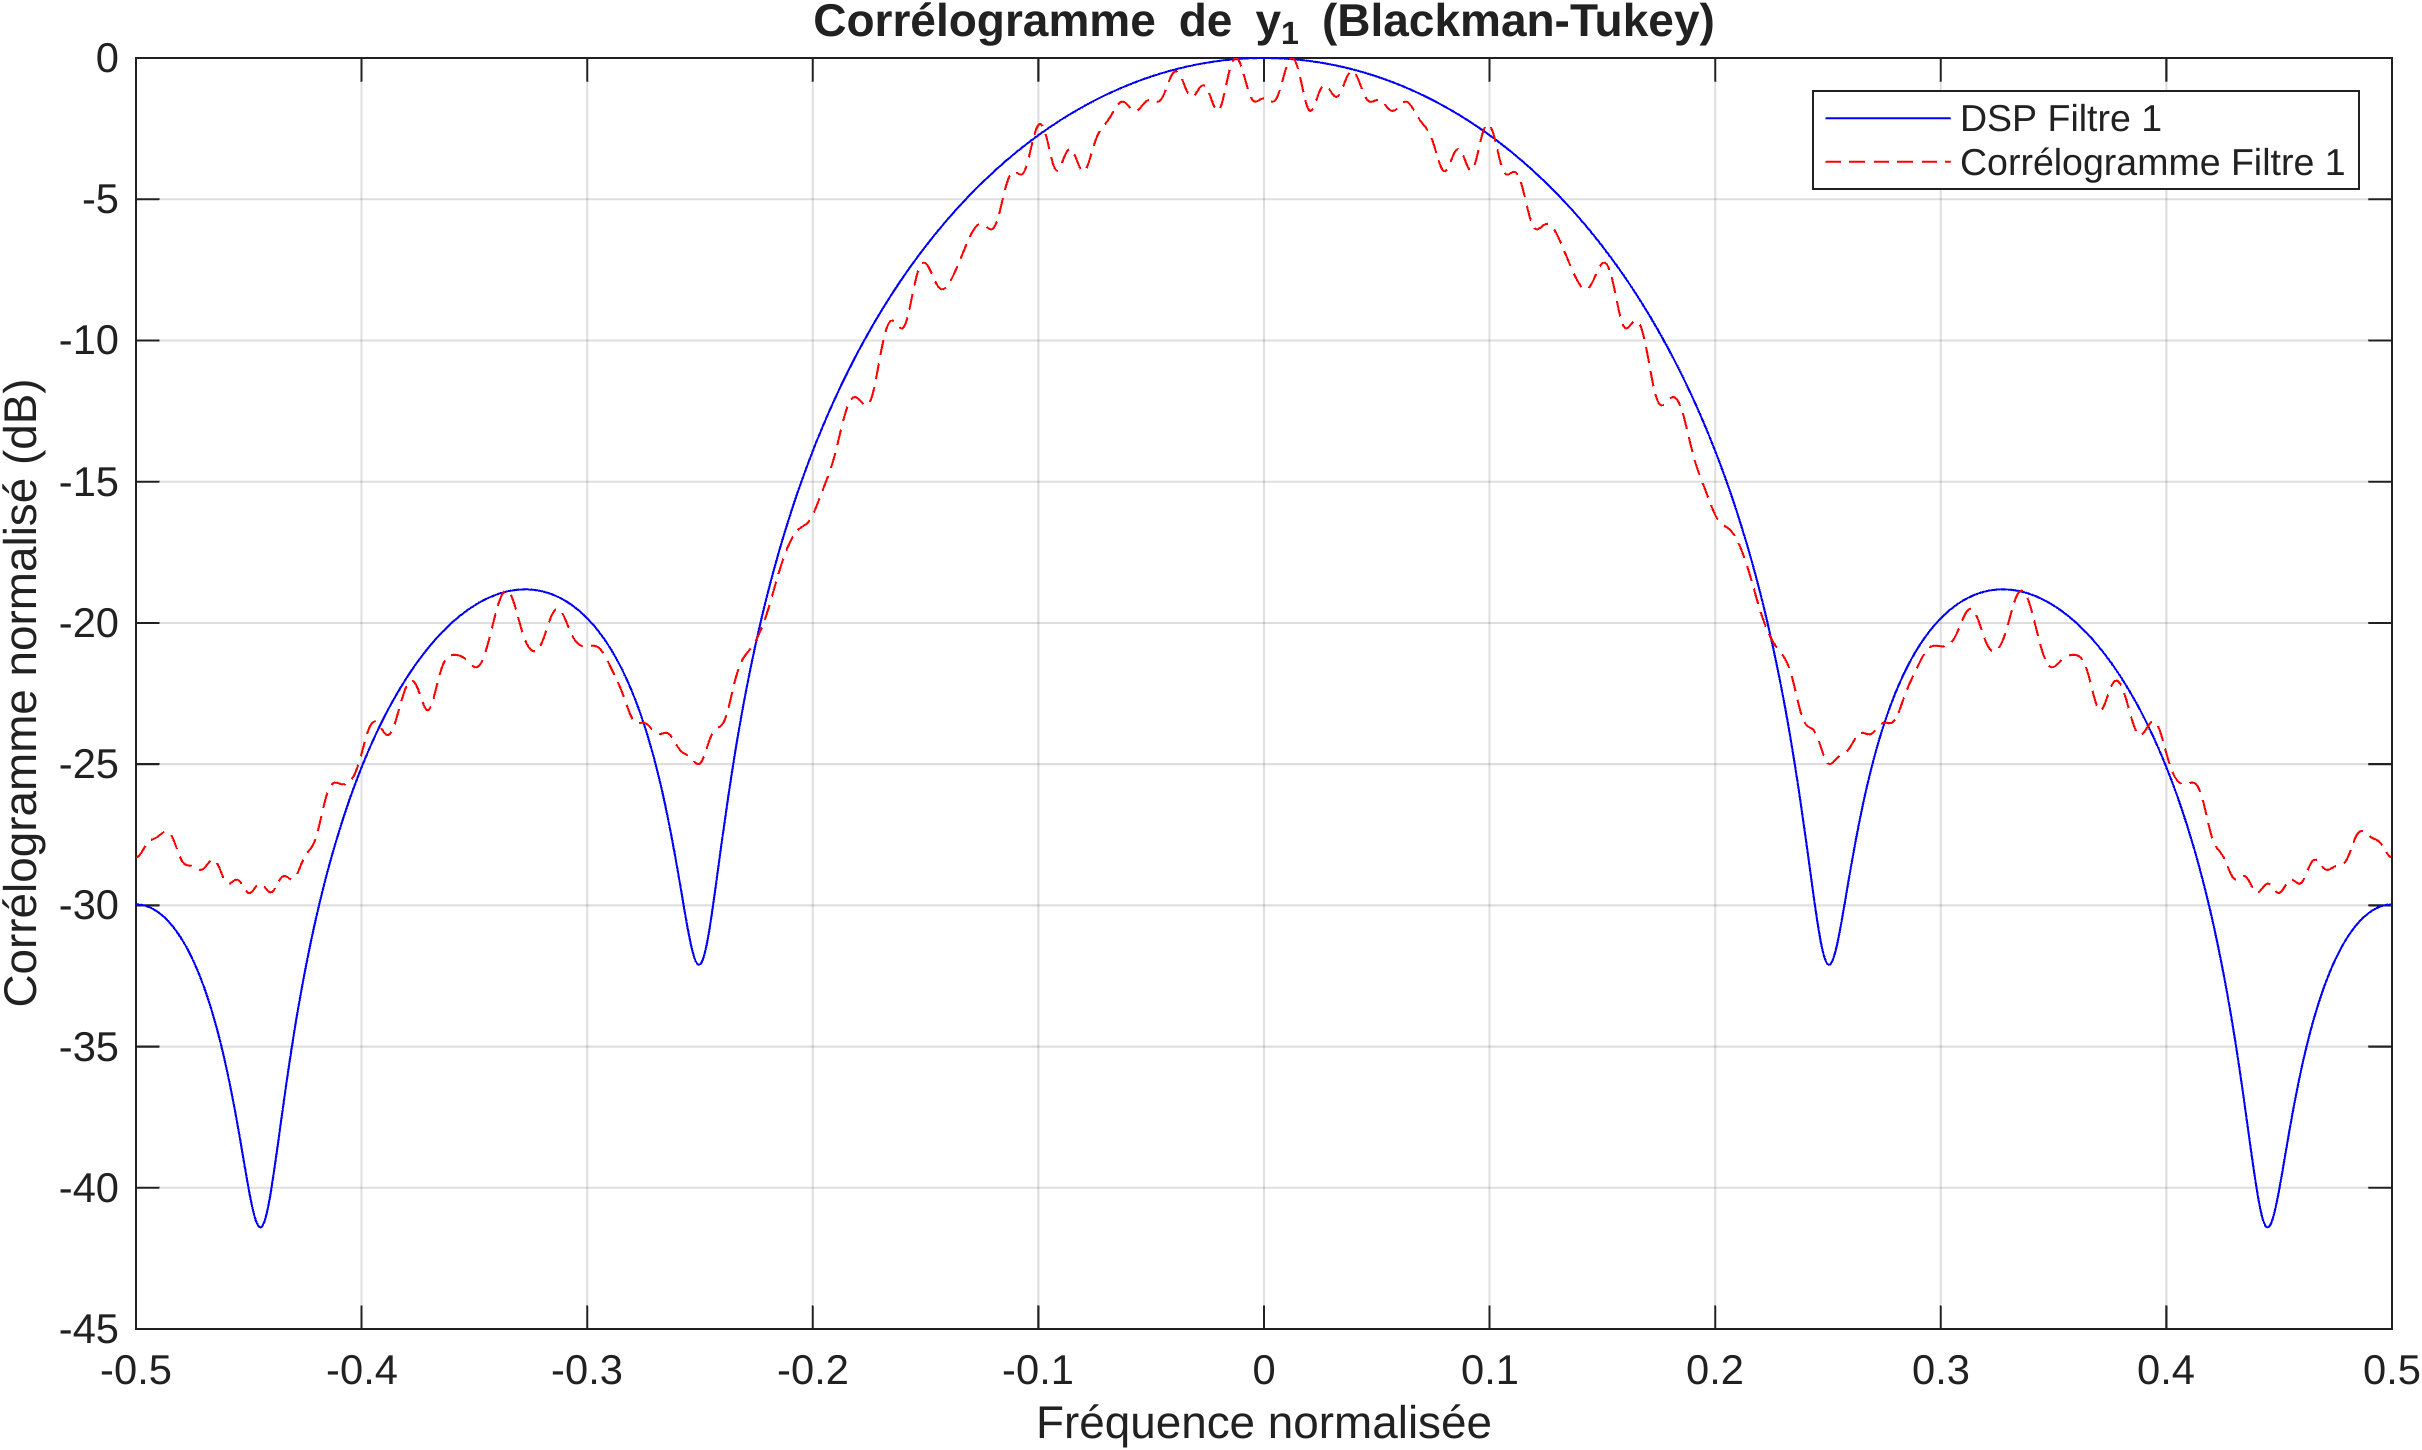
\includegraphics[width=\linewidth]{fig13.png}
    \caption{MA(4)}
  \end{subfigure}
  \begin{subfigure}{0.43\linewidth}
    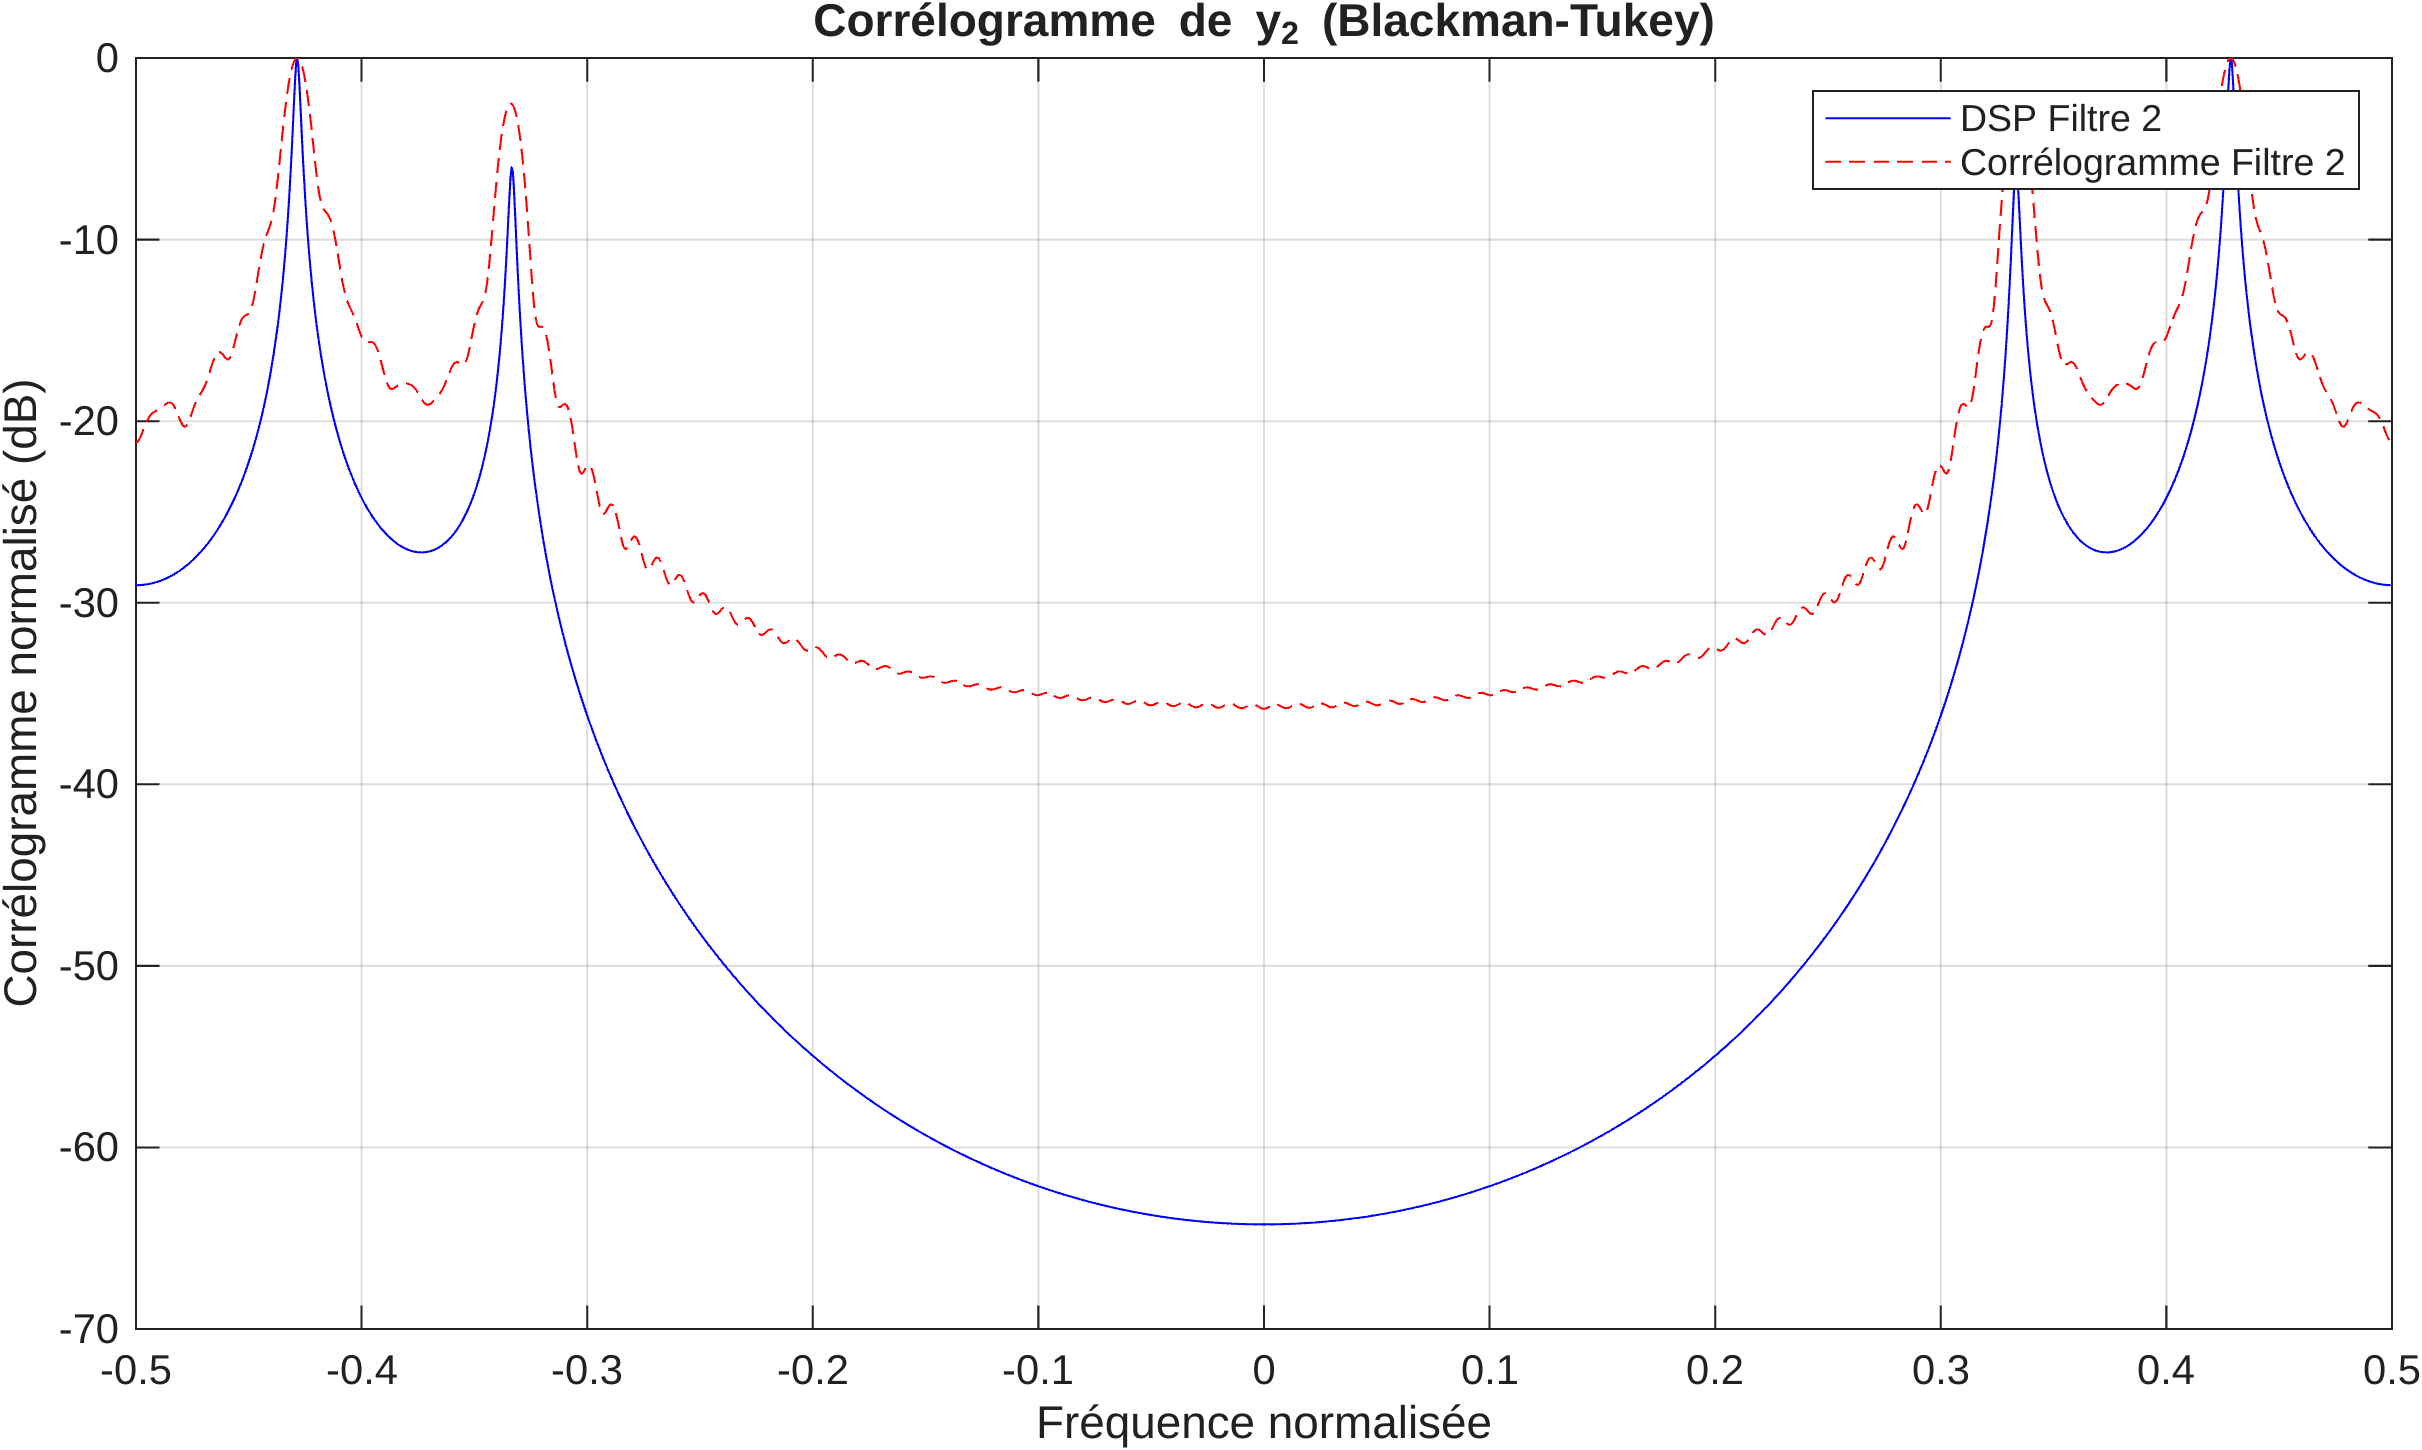
\includegraphics[width=\linewidth]{fig14.png}
    \caption{AR(4)}
  \end{subfigure}
  \caption{Corrélogrammes ($K_{\max} = 100$, fenêtre triangulaire) comparés à la DSP théorique.}
  \label{fig:correlo}
\end{figure}

\subsubsection{Synthèse}

Le tableau~\ref{tab:synthese} résume les paramètres retenus. Aucun estimateur n'est uniformément meilleur. Le périodogramme de Welch offre le meilleur compromis entre résolution, variance et fuite spectrale, mais la finesse des pics de l'AR(4) impose dans tous les cas un faible nombre de moyennes, donc une variance élevée. Pour un tel processus, dont le modèle est connu, un estimateur paramétrique (identification des coefficients $a_i$ par les équations de Yule-Walker) serait plus adapté que les méthodes non paramétriques.

\begin{table}[ht]
  \centering
  \begin{tabular}{lllll}
    \toprule
    Méthode & Paramètres MA(4) & Var. MA(4) & Paramètres AR(4) & Var. AR(4) \\
    \midrule
    Daniell & $2m+1 = 33$ & $S_x^2/33$ & $2m+1 = 5$ & $S_x^2/5$ \\
    Bartlett & $L = 80$, $K = 25$ & $S_x^2/25$ & $L = 400$, $K = 5$ & $S_x^2/5$ \\
    Welch (Hann, 50~\%) & $L = 100$, $K = 39$ & $\approx S_x^2/37$ & $L = 500$, $K = 7$ & $\approx S_x^2/6{,}7$ \\
    Corrélogramme (triangle) & $K_{\max} = 100$ & $\approx S_x^2/30$ & $K_{\max} = 100$ & $\approx S_x^2/30$ \\
    \bottomrule
  \end{tabular}
  \caption{Paramètres des estimateurs et réduction de variance approchée par rapport au périodogramme.}
  \label{tab:synthese}
\end{table}

%=====================================================================
\section{Méthode d'extraction du marqueur}
\label{sec:methode}
%=====================================================================

Dans cette section, conformément au sujet, $x(n)$ désigne un signal de $M$ échantillons, $N$ la taille des blocs ou la longueur des filtres, et $L = \lfloor M/N \rfloor$ le nombre de blocs. Les figures sont obtenues pour un bruit blanc gaussien, avec $M = 2000$ et $N = 200$.

\subsection{Étape 1 : centrage et intégration}

Le signal est centré puis intégré :
\begin{equation}
  y(n) = \sum_{k=1}^{n} \big( x(k) - \bar{x} \big), \qquad \bar{x} = \frac{1}{M} \sum_{k=1}^{M} x(k).
  \label{eq:integration}
\end{equation}
L'intégration est un filtrage par $1/(1-z^{-1})$, dont le pôle se trouve sur le cercle unité : $y$ n'est pas stationnaire. Pour un bruit blanc, $y$ est une marche aléatoire de variance $\operatorname{Var}[y(n)] = n\,\sigma_x^2$, qui croît sans borne. C'est cette composante lentement variable que les étapes suivantes cherchent à décrire. Le centrage préalable garantit en outre $y(M) = 0$ : le profil part de 0 et y revient, comme on l'observe sur les figures~\ref{fig:tendances} et~\ref{fig:strategies}.

\subsection{Étape 2 : estimation de la tendance}

\paragraph{2a. Régression polynomiale par blocs.}
Le profil est découpé en $L$ blocs de $N$ échantillons, $y_l(n) = y\big((l-1)N + n\big)$ pour $n = 1, \dots, N$. Les échantillons au-delà de $LN$ sont ignorés. Sur chaque bloc, la tendance est modélisée par un polynôme de degré $d$ : $d = 0$ (moyenne), $d = 1$ (droite de régression) ou $d = 2, 3$. Sous forme matricielle :
\begin{equation}
  \mathbf{y}_l = \mathbf{A}\, \boldsymbol{\theta}_l + \mathbf{e}_l,
  \qquad
  \mathbf{A} =
  \begin{pmatrix}
    1 & 1 & \cdots & 1^d \\
    1 & 2 & \cdots & 2^d \\
    \vdots & \vdots & & \vdots \\
    1 & N & \cdots & N^d
  \end{pmatrix},
  \label{eq:modele}
\end{equation}
où $\boldsymbol{\theta}_l \in \mathbb{R}^{d+1}$ regroupe les coefficients du polynôme et $\mathbf{e}_l$ l'écart au modèle. L'approche vue en cours est celle des \emph{moindres carrés}. On minimise $J(\boldsymbol{\theta}) = \|\mathbf{y}_l - \mathbf{A}\boldsymbol{\theta}\|^2$ ; en annulant le gradient $-2\mathbf{A}^T(\mathbf{y}_l - \mathbf{A}\boldsymbol{\theta})$, on obtient les équations normales, puis :
\begin{equation}
  \hat{\boldsymbol{\theta}}_l = \left(\mathbf{A}^T \mathbf{A}\right)^{-1} \mathbf{A}^T \mathbf{y}_l,
  \qquad
  \hat{\mathbf{t}}_l = \mathbf{A}\hat{\boldsymbol{\theta}}_l = \underbrace{\mathbf{A}\left(\mathbf{A}^T \mathbf{A}\right)^{-1} \mathbf{A}^T}_{\boldsymbol{\Pi}} \mathbf{y}_l.
  \label{eq:mc}
\end{equation}
$\mathbf{A}^T\mathbf{A}$ est inversible dès que $N \geq d+1$ (colonnes de $\mathbf{A}$ linéairement indépendantes). La tendance estimée est la projection orthogonale $\boldsymbol{\Pi}\mathbf{y}_l$ du bloc sur le sous-espace des polynômes de degré $d$ ; si $\mathbf{e}_l$ est blanc et gaussien, elle coïncide avec l'estimateur du maximum de vraisemblance. Pour $d = 0$, on retrouve la moyenne du bloc ; pour $d = 1$, la pente $\sum (n - \bar{n})(y_l(n) - \bar{y}_l) / \sum (n-\bar{n})^2$ utilisée dans le code.

Deux remarques pratiques s'imposent. D'une part, $\mathbf{A}^T\mathbf{A}$ est mal conditionnée : ses coefficients vont de $N$ à $\sum n^{2d} \sim N^{2d+1}$, soit environ $10^{15}$ pour $d = 3$ et $N = 200$. Le code évite donc l'inversion explicite au profit d'une factorisation QR (opérateur \texttt{\textbackslash} de MATLAB) et, dans la fonction \texttt{marqueur}, remplace $n$ par $n/N$. D'autre part, si $N = d+1$, le polynôme passe par tous les points du bloc et le résidu est nul : il faut $N \geq d+2$.

Sur la figure~\ref{fig:tendances}, la tendance globale obtenue par concaténation est discontinue aux frontières des blocs. Plus $d$ est grand, plus le polynôme suit les fluctuations rapides : pour $d = 3$, il épouse presque la marche aléatoire et « absorbe » une partie des fluctuations que l'on cherche à mesurer, ce qui diminue la puissance résiduelle de l'étape~3.

\begin{figure}[!htb]
  \centering
  \begin{subfigure}{0.43\linewidth}
    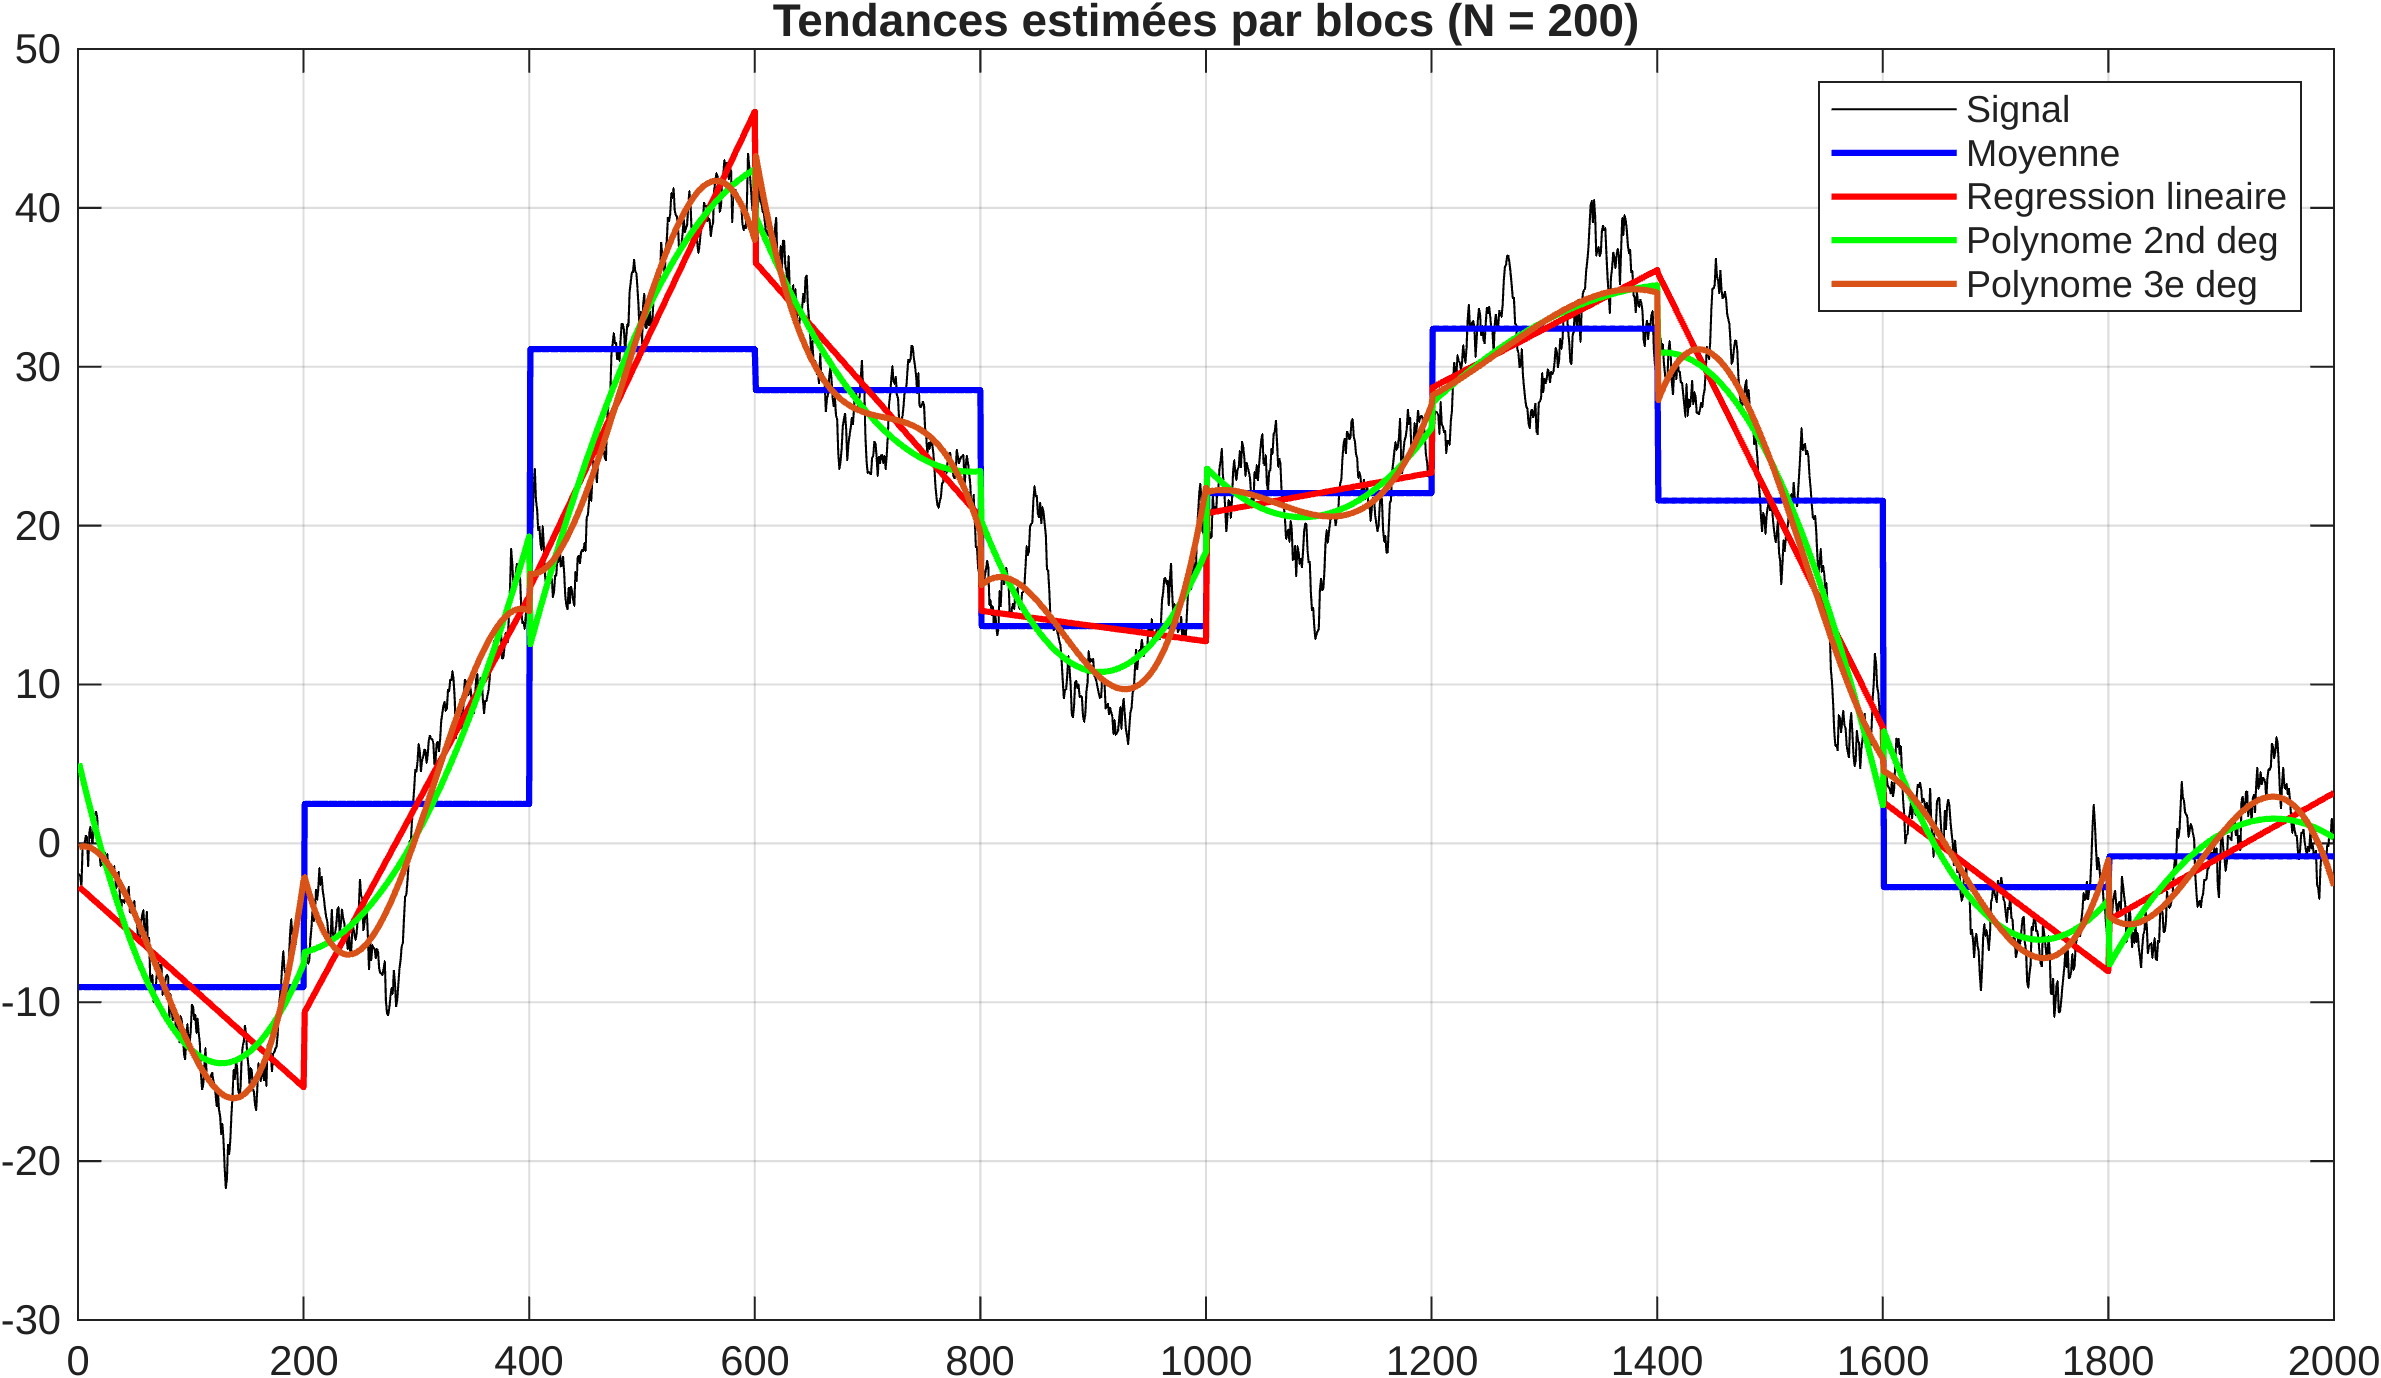
\includegraphics[width=\linewidth]{fig15.png}
    \caption{2a : régression par blocs, $d = 0$ à 3}
    \label{fig:tendances}
  \end{subfigure}
  \begin{subfigure}{0.43\linewidth}
    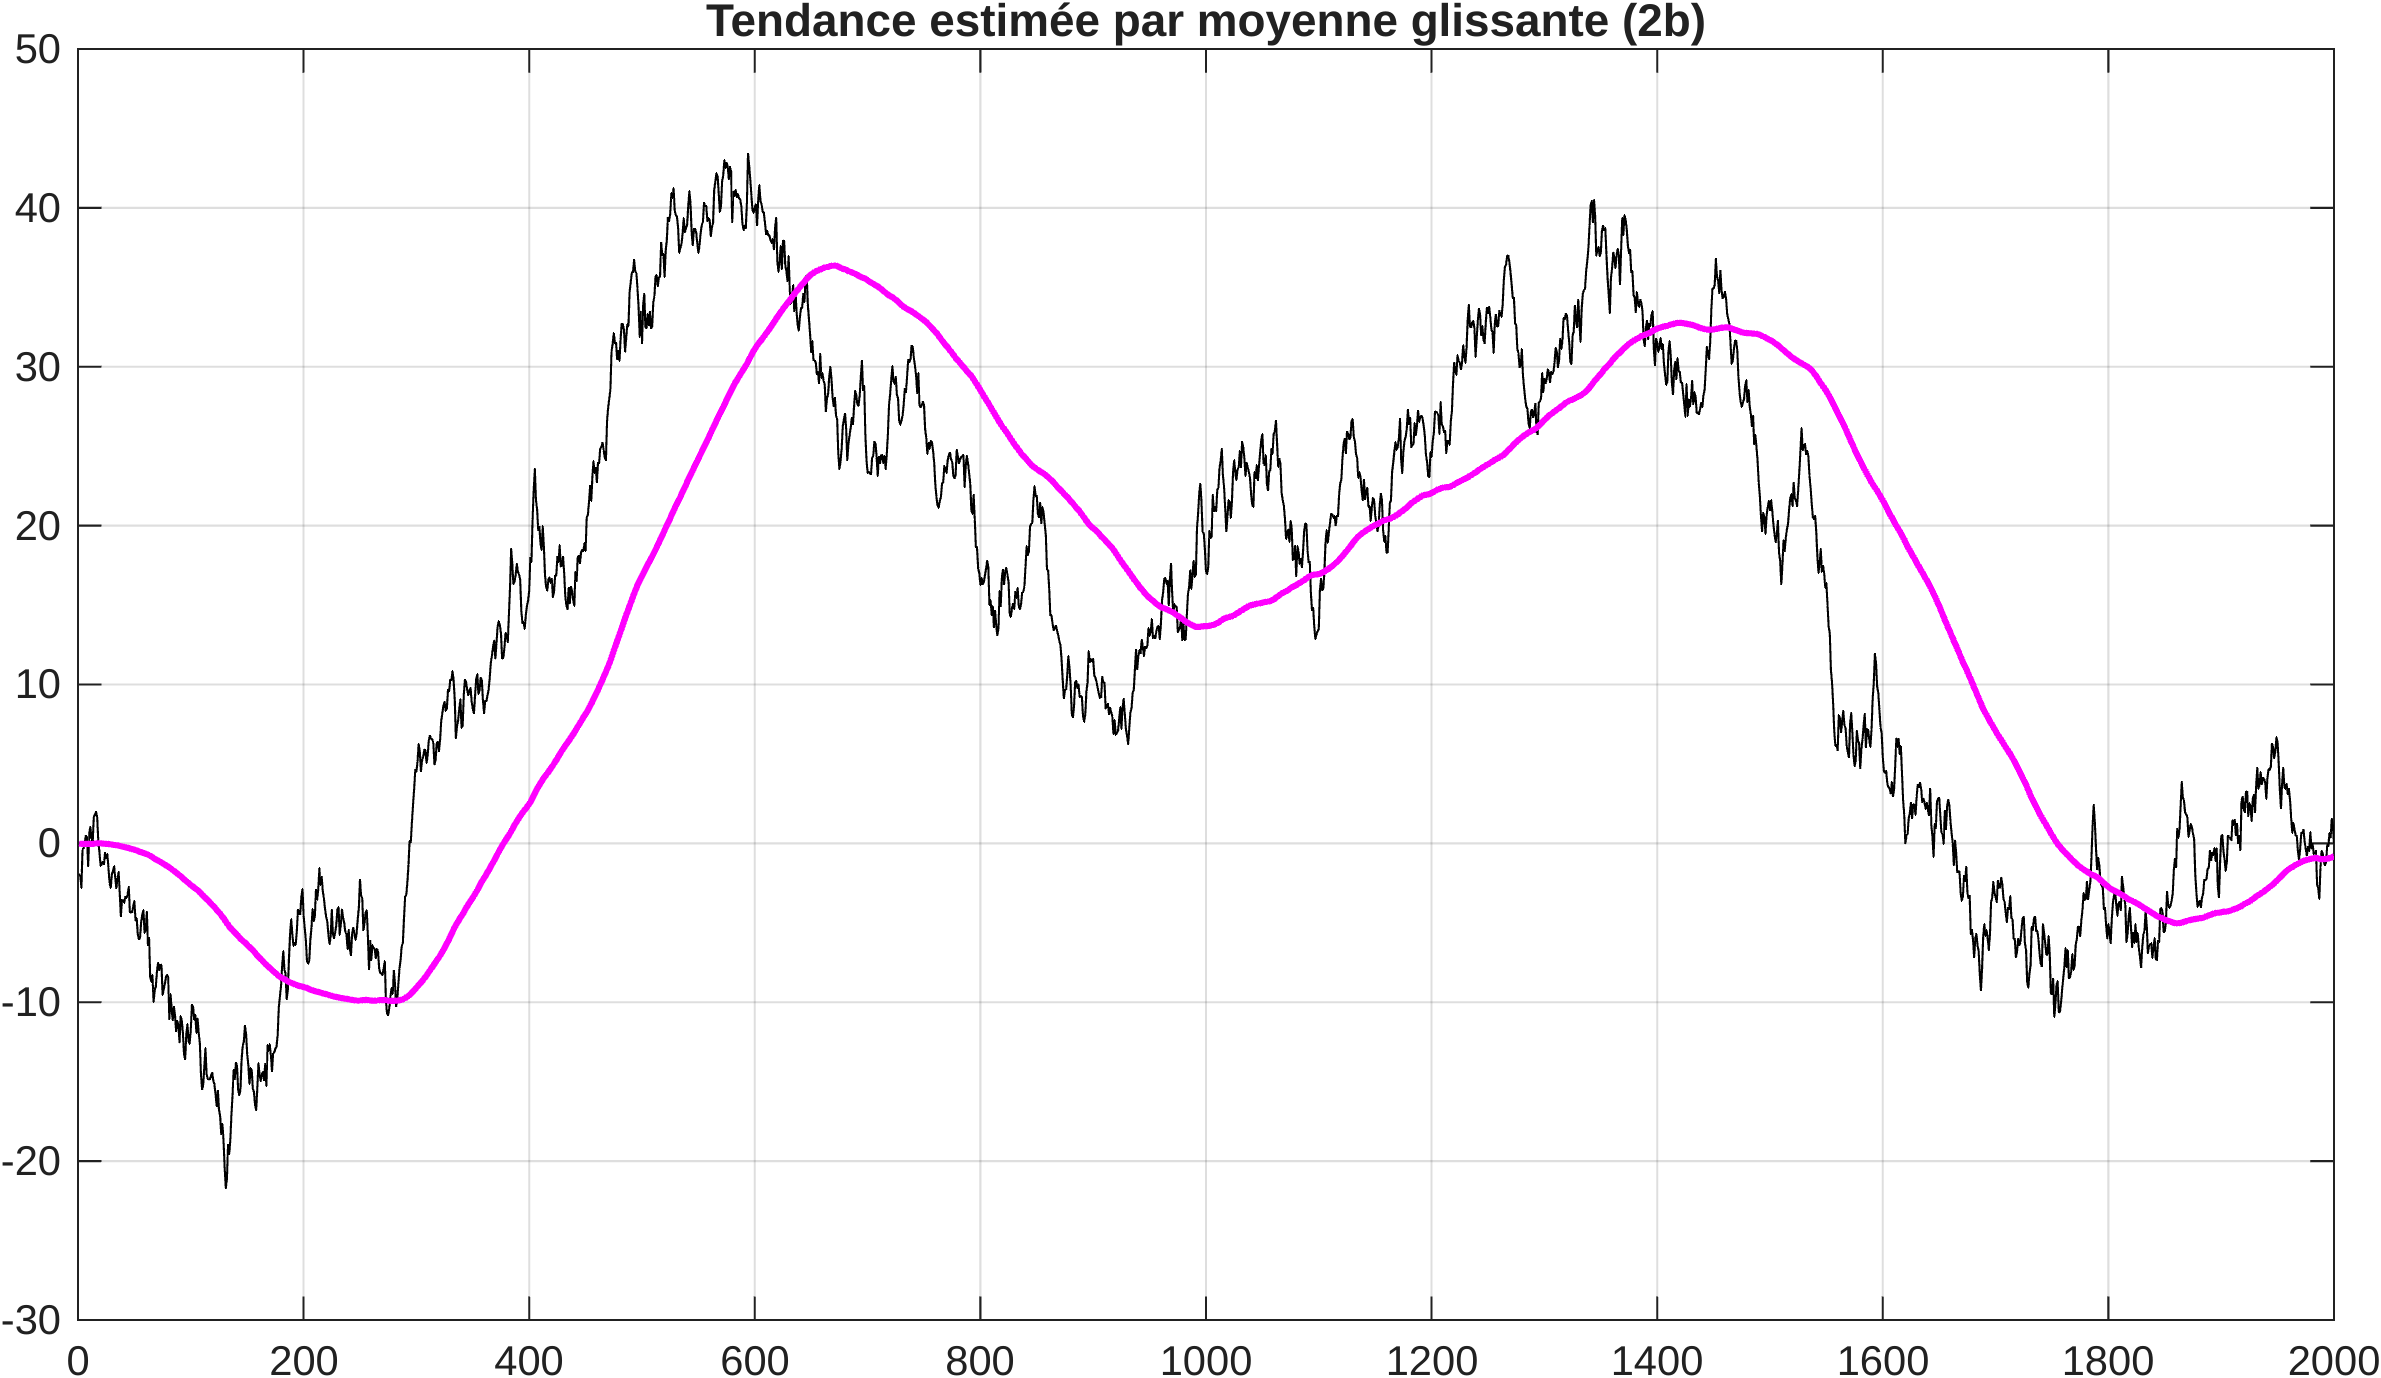
\includegraphics[width=\linewidth]{fig16.png}
    \caption{2b : moyenne glissante causale}
    \label{fig:mg}
  \end{subfigure}
  \caption{Tendances estimées sur le profil d'un bruit blanc intégré ($M = 2000$, $N = 200$).}
\end{figure}

\paragraph{2b. Filtrage passe-bas par moyenne glissante.}
La tendance est estimée par la moyenne des $N$ derniers échantillons :
\begin{equation}
  t(n) = \frac{1}{N} \sum_{k=0}^{N-1} y(n-k) = (h * y)(n),
  \qquad
  h(n) =
  \begin{cases}
    1/N & 0 \leq n \leq N-1,\\
    0 & \text{sinon.}
  \end{cases}
  \label{eq:mg}
\end{equation}
Le filtre ainsi défini présente les caractéristiques suivantes :
\begin{itemize}
  \item \textbf{RIF}, puisque $h$ est à support fini. L'écriture $H(z) = \frac{1}{N}\frac{1 - z^{-N}}{1 - z^{-1}}$ suggère une implantation récursive, $t(n) = t(n-1) + \big(y(n) - y(n-N)\big)/N$ : le pôle en $z = 1$ y est compensé par un zéro, mais les erreurs d'arrondi s'accumulent ;
  \item \textbf{causal}, car $h(n) = 0$ pour $n < 0$, et \textbf{stable}, car $\sum_n |h(n)| = 1$, comme tout filtre RIF ;
  \item \textbf{réponse en fréquence} :
  \begin{equation}
    H(\nu) = \frac{1}{N} \sum_{n=0}^{N-1} e^{-j2\pi\nu n} = e^{-j\pi\nu(N-1)}\, \frac{\sin(\pi\nu N)}{N \sin(\pi\nu)}.
    \label{eq:H_mg}
  \end{equation}
  C'est un passe-bas de gain unité en $\nu = 0$, de coupure à $-3$~dB d'environ $0{,}44/N$ ($2{,}2 \cdot 10^{-3}$ pour $N = 200$), de premier zéro en $1/N$, et dont les lobes secondaires à $-13$~dB en font un passe-bas médiocre ;
  \item \textbf{phase linéaire}, car $h$ est symétrique par rapport à $(N-1)/2$ : $\varphi(\nu) = -\pi\nu(N-1)$, à des sauts de $\pi$ près. Le temps de propagation de groupe est constant : $\tau = (N-1)/2$ échantillons ;
  \item \textbf{pas à minimum de phase} : les zéros de $H(z)$, $z_k = e^{j2\pi k/N}$ pour $k = 1, \dots, N-1$, sont sur le cercle unité et non strictement à l'intérieur, si bien que le filtre n'admet pas d'inverse stable.
\end{itemize}
Le retard $\tau = 99{,}5$ échantillons est nettement visible sur la figure~\ref{fig:mg}, de même que le transitoire initial : la tendance part de 0, car les $N-1$ premiers échantillons sont moyennés avec des valeurs nulles. Ce retard pénalise l'estimation : à l'étape~3, le résidu contiendrait l'erreur $y(n) - y(n - \tau)$, sans rapport avec les fluctuations locales. D'où l'intérêt d'un filtrage à phase nulle.

\paragraph{2c. Filtrage à phase nulle.}
On note $Y(\nu)$, $H(\nu)$ les transformées de Fourier de $y$ et $h$, toutes deux réelles. Pour un signal réel, le retournement temporel conjugue la transformée de Fourier : $y(-n) \leftrightarrow Y^*(\nu)$.

\emph{Stratégie 1.} On a successivement $g = h * y \leftrightarrow H Y$, puis $g(-n) \leftrightarrow H^* Y^*$, puis $r = h * g(-n) \leftrightarrow H H^* Y^*$. La sortie finale vérifie donc :
\begin{equation}
  r(-n) \;\leftrightarrow\; \big(H H^* Y^*\big)^* = |H(\nu)|^2\, Y(\nu).
  \label{eq:strat1}
\end{equation}
Le filtre équivalent $|H(\nu)|^2$ est réel et positif : la stratégie~1 est à phase nulle \emph{pour tout filtre $h$ réel}. Sa réponse impulsionnelle est l'autocorrélation de $h$, paire, et le gain en décibels est doublé, ce qui renforce l'atténuation. Avec la moyenne glissante, elle devient une fenêtre triangulaire de $2N-1$ points.

\emph{Stratégie 2.} On a $g = h * y \leftrightarrow H Y$, puis $r = h * y(-n) \leftrightarrow H Y^*$, donc $r(-n) \leftrightarrow H^* Y$. Avec le facteur $1/2$ ajouté dans le code pour conserver un gain unité en $\nu = 0$ :
\begin{equation}
  \tfrac{1}{2}\big(g(n) + r(-n)\big) \;\leftrightarrow\; \tfrac{1}{2}\big(H(\nu) + H^*(\nu)\big)\, Y(\nu) = \operatorname{Re}\{H(\nu)\}\, Y(\nu).
  \label{eq:strat2}
\end{equation}
Le filtre équivalent est la partie paire $\frac{1}{2}\big(h(n) + h(-n)\big)$ de $h$ et sa réponse $\operatorname{Re}\{H(\nu)\}$ est réelle. La phase vaut donc 0 là où $\operatorname{Re}\{H\} > 0$, mais $\pi$ là où $\operatorname{Re}\{H\} < 0$. La stratégie~2 n'est à phase nulle que si $h$ est réel \emph{et} si $\operatorname{Re}\{H(\nu)\} \geq 0$ sur la bande utile. Pour la moyenne glissante, d'après~\eqref{eq:H_mg} :
\begin{equation}
  \operatorname{Re}\{H(\nu)\} = \cos\big(\pi\nu(N-1)\big)\, \frac{\sin(\pi\nu N)}{N\sin(\pi\nu)},
\end{equation}
qui change de signe dès $\nu = 1/(2(N-1))$, soit avant le premier zéro $1/N$. La coupure est environ divisée par deux par rapport à la stratégie~1, et certaines composantes sont inversées. Pour réaliser exactement une réponse paire $g(n)$ donnée, il faut au contraire choisir pour $h$ sa « moitié causale » : $h(0) = g(0)$, $h(n) = 2g(n)$ pour $n \geq 1$ et $h(n) = 0$ pour $n < 0$.

\emph{Choix de $h$ et observations.} La tendance est le contenu basse fréquence du profil : $h$ doit être un passe-bas, de coupure de l'ordre de $1/N$ pour être comparable à la méthode par blocs. Nous avons retenu la moyenne glissante de 2b, et la figure~\ref{fig:strategies} le confirme :
\begin{itemize}
  \item avec la stratégie~1, le passe-bas fournit une tendance lisse et sans retard, contrairement à la figure~\ref{fig:mg} ; avec la stratégie~2, elle est plus aplatie (maximum vers 30 au lieu de 34 autour de $n = 600$), conformément à sa coupure plus basse ;
  \item le passe-haut et le passe-bande donnent des oscillations autour de 0 : ils extraient les \emph{détails} du profil, c'est-à-dire une approximation du résidu, et non la tendance. Le coupe-bande laisse passer les hautes fréquences et fournit une tendance bruitée ; avec la stratégie~2, ce filtre causal de retard 100 donne même $\operatorname{Re}\{H(\nu)\} = A(\nu)\cos(200\pi\nu)$, une réponse fortement modulée ;
  \item sur un signal de longueur finie, les deux passages du filtre créent des transitoires aux deux extrémités : les $N-1$ premiers et derniers échantillons ne sont pas fiables. La fonction \texttt{filtfilt} de MATLAB met en œuvre la stratégie~1 avec un traitement des conditions initiales qui réduit cet effet.
\end{itemize}

\begin{figure}[!htb]
  \centering
  \begin{subfigure}{0.43\linewidth}
    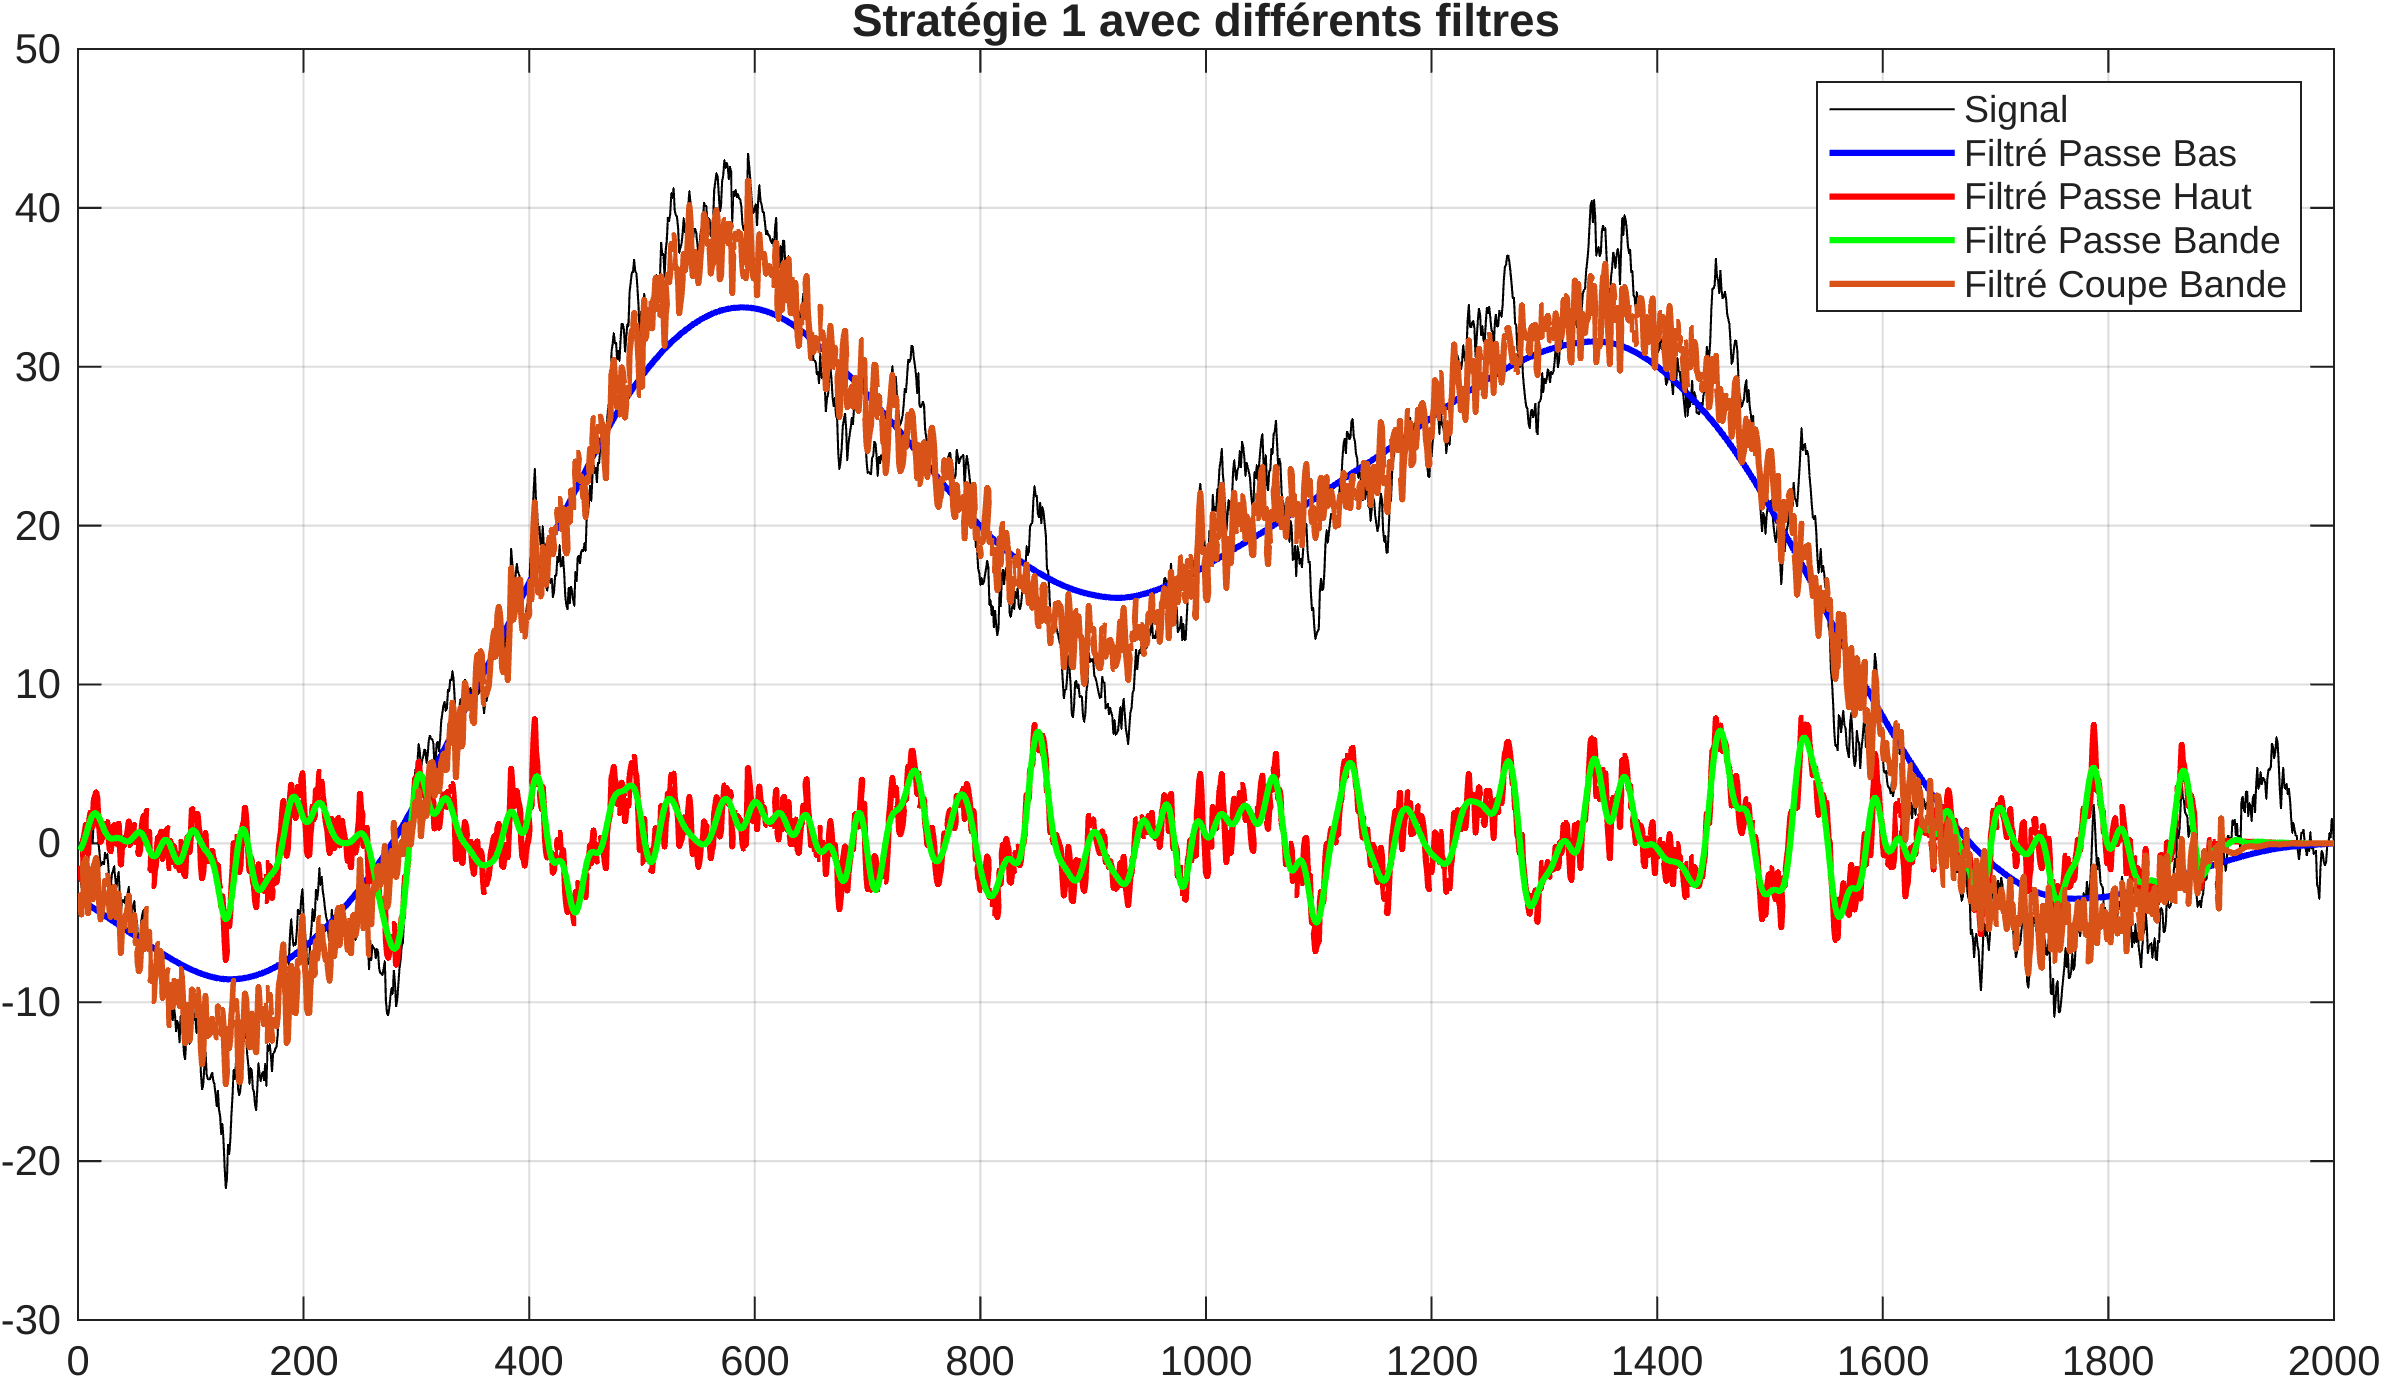
\includegraphics[width=\linewidth]{fig17.png}
    \caption{Stratégie 1}
  \end{subfigure}
  \begin{subfigure}{0.43\linewidth}
    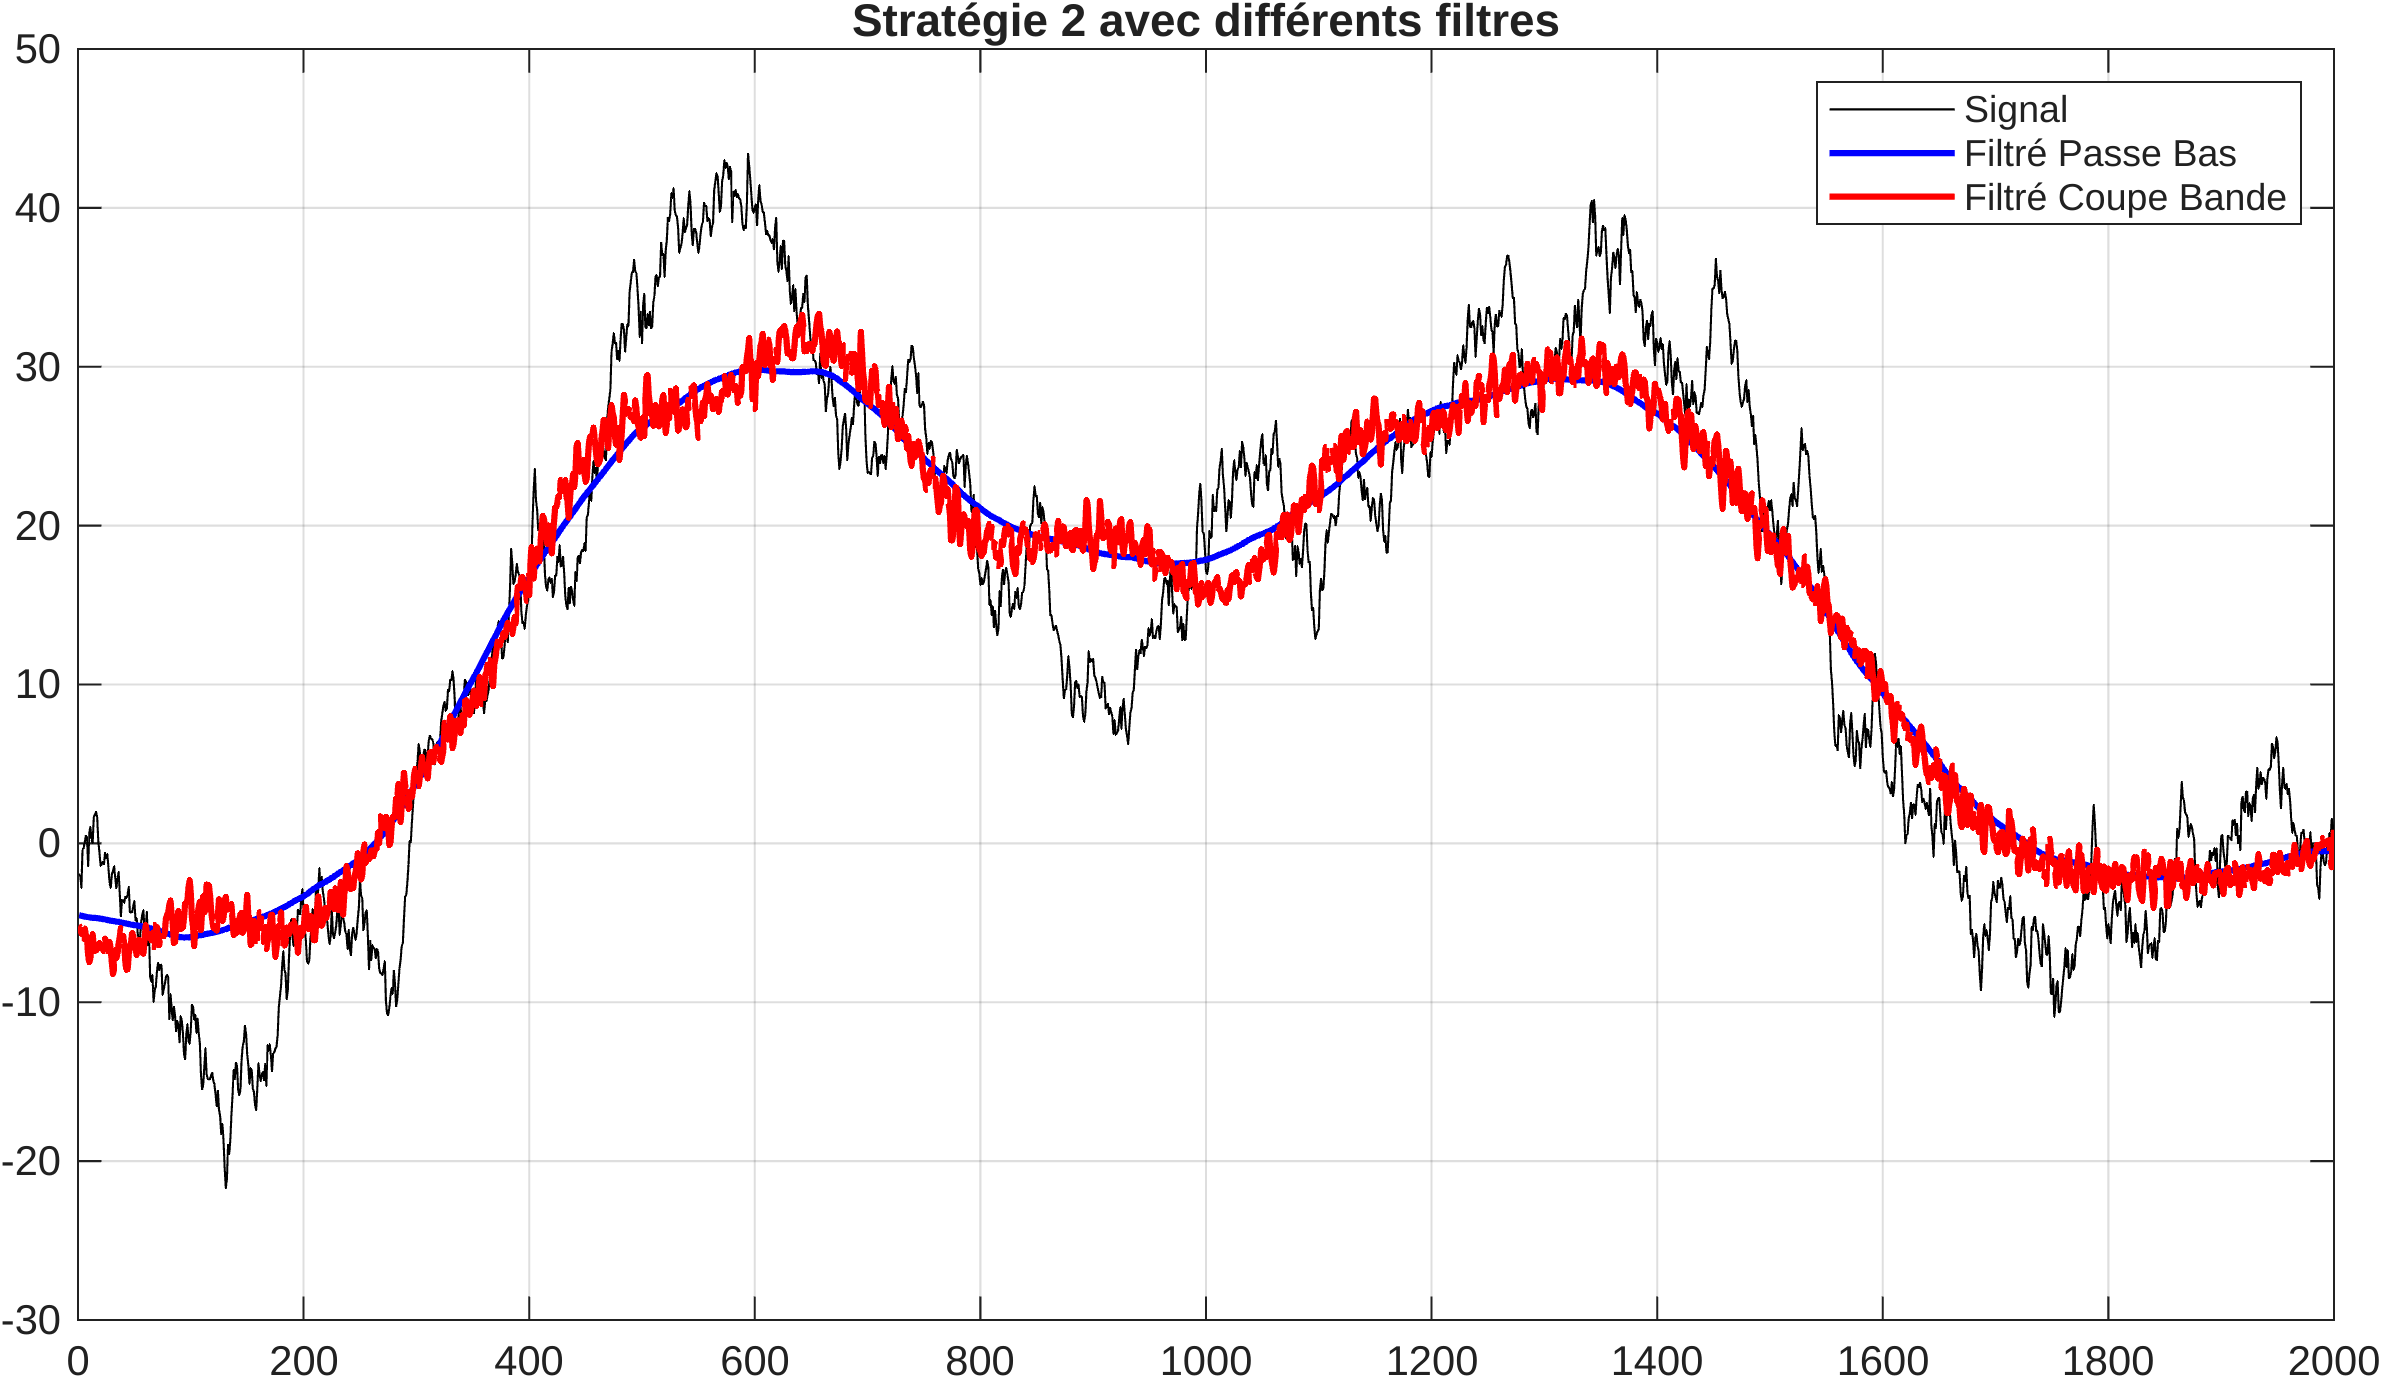
\includegraphics[width=\linewidth]{fig18.png}
    \caption{Stratégie 2}
  \end{subfigure}
  \caption{Filtrage à phase nulle du profil ($N = 200$) avec différents filtres $h$.}
  \label{fig:strategies}
\end{figure}

\subsection{Étape 3 : résidu et puissance}

La tendance globale $t(n)$ est retranchée au profil, ce qui donne le résidu $r(n) = y(n) - t(n)$. Sa puissance moyenne vaut, pour la méthode par blocs :
\begin{equation}
  P(N) = \frac{1}{LN} \sum_{n=1}^{LN} r^2(n) = \frac{1}{LN} \sum_{l=1}^{L} \big\| (\mathbf{I} - \boldsymbol{\Pi})\, \mathbf{y}_l \big\|^2.
  \label{eq:PN}
\end{equation}
Pour les méthodes par filtrage, la somme doit exclure les échantillons affectés par les transitoires. Ce calcul conduit à un résultat utile pour la suite. Si l'on applique l'étape~2 directement à un bruit blanc $x$ de variance $\sigma^2$, sans intégration, la projection $\mathbf{I} - \boldsymbol{\Pi}$ sur un sous-espace de dimension $N - (d+1)$ donne :
\begin{equation}
  \mathbb{E}\big[P(N)\big] = \sigma^2 \left( 1 - \frac{d+1}{N} \right).
  \label{eq:PN_bb}
\end{equation}

\subsection{Étape 4 : représentation log-log et marqueur}

Pour $N$ variant de 3 à $M/2$, les couples $\big(\ln N, \ln P(N)\big)$ sont ajustés par une droite au sens des moindres carrés, c'est-à-dire par le modèle~\eqref{eq:modele} avec $d = 1$. Sa pente $a$ constitue le marqueur. Si $P(N) \propto N^{2\alpha}$, alors $a = 2\alpha$, où $\alpha$ est l'exposant de fluctuation de la DFA~[5,6] :
\begin{itemize}
  \item pour un bruit blanc intégré, la marche aléatoire vérifie $P(N) \propto N$, d'où $\alpha = 0{,}5$ et $a = 1$ ;
  \item $\alpha > 0{,}5$ traduit des corrélations à longue portée et $\alpha < 0{,}5$ des anticorrélations.
\end{itemize}

\begin{figure}[!htb]
  \centering
  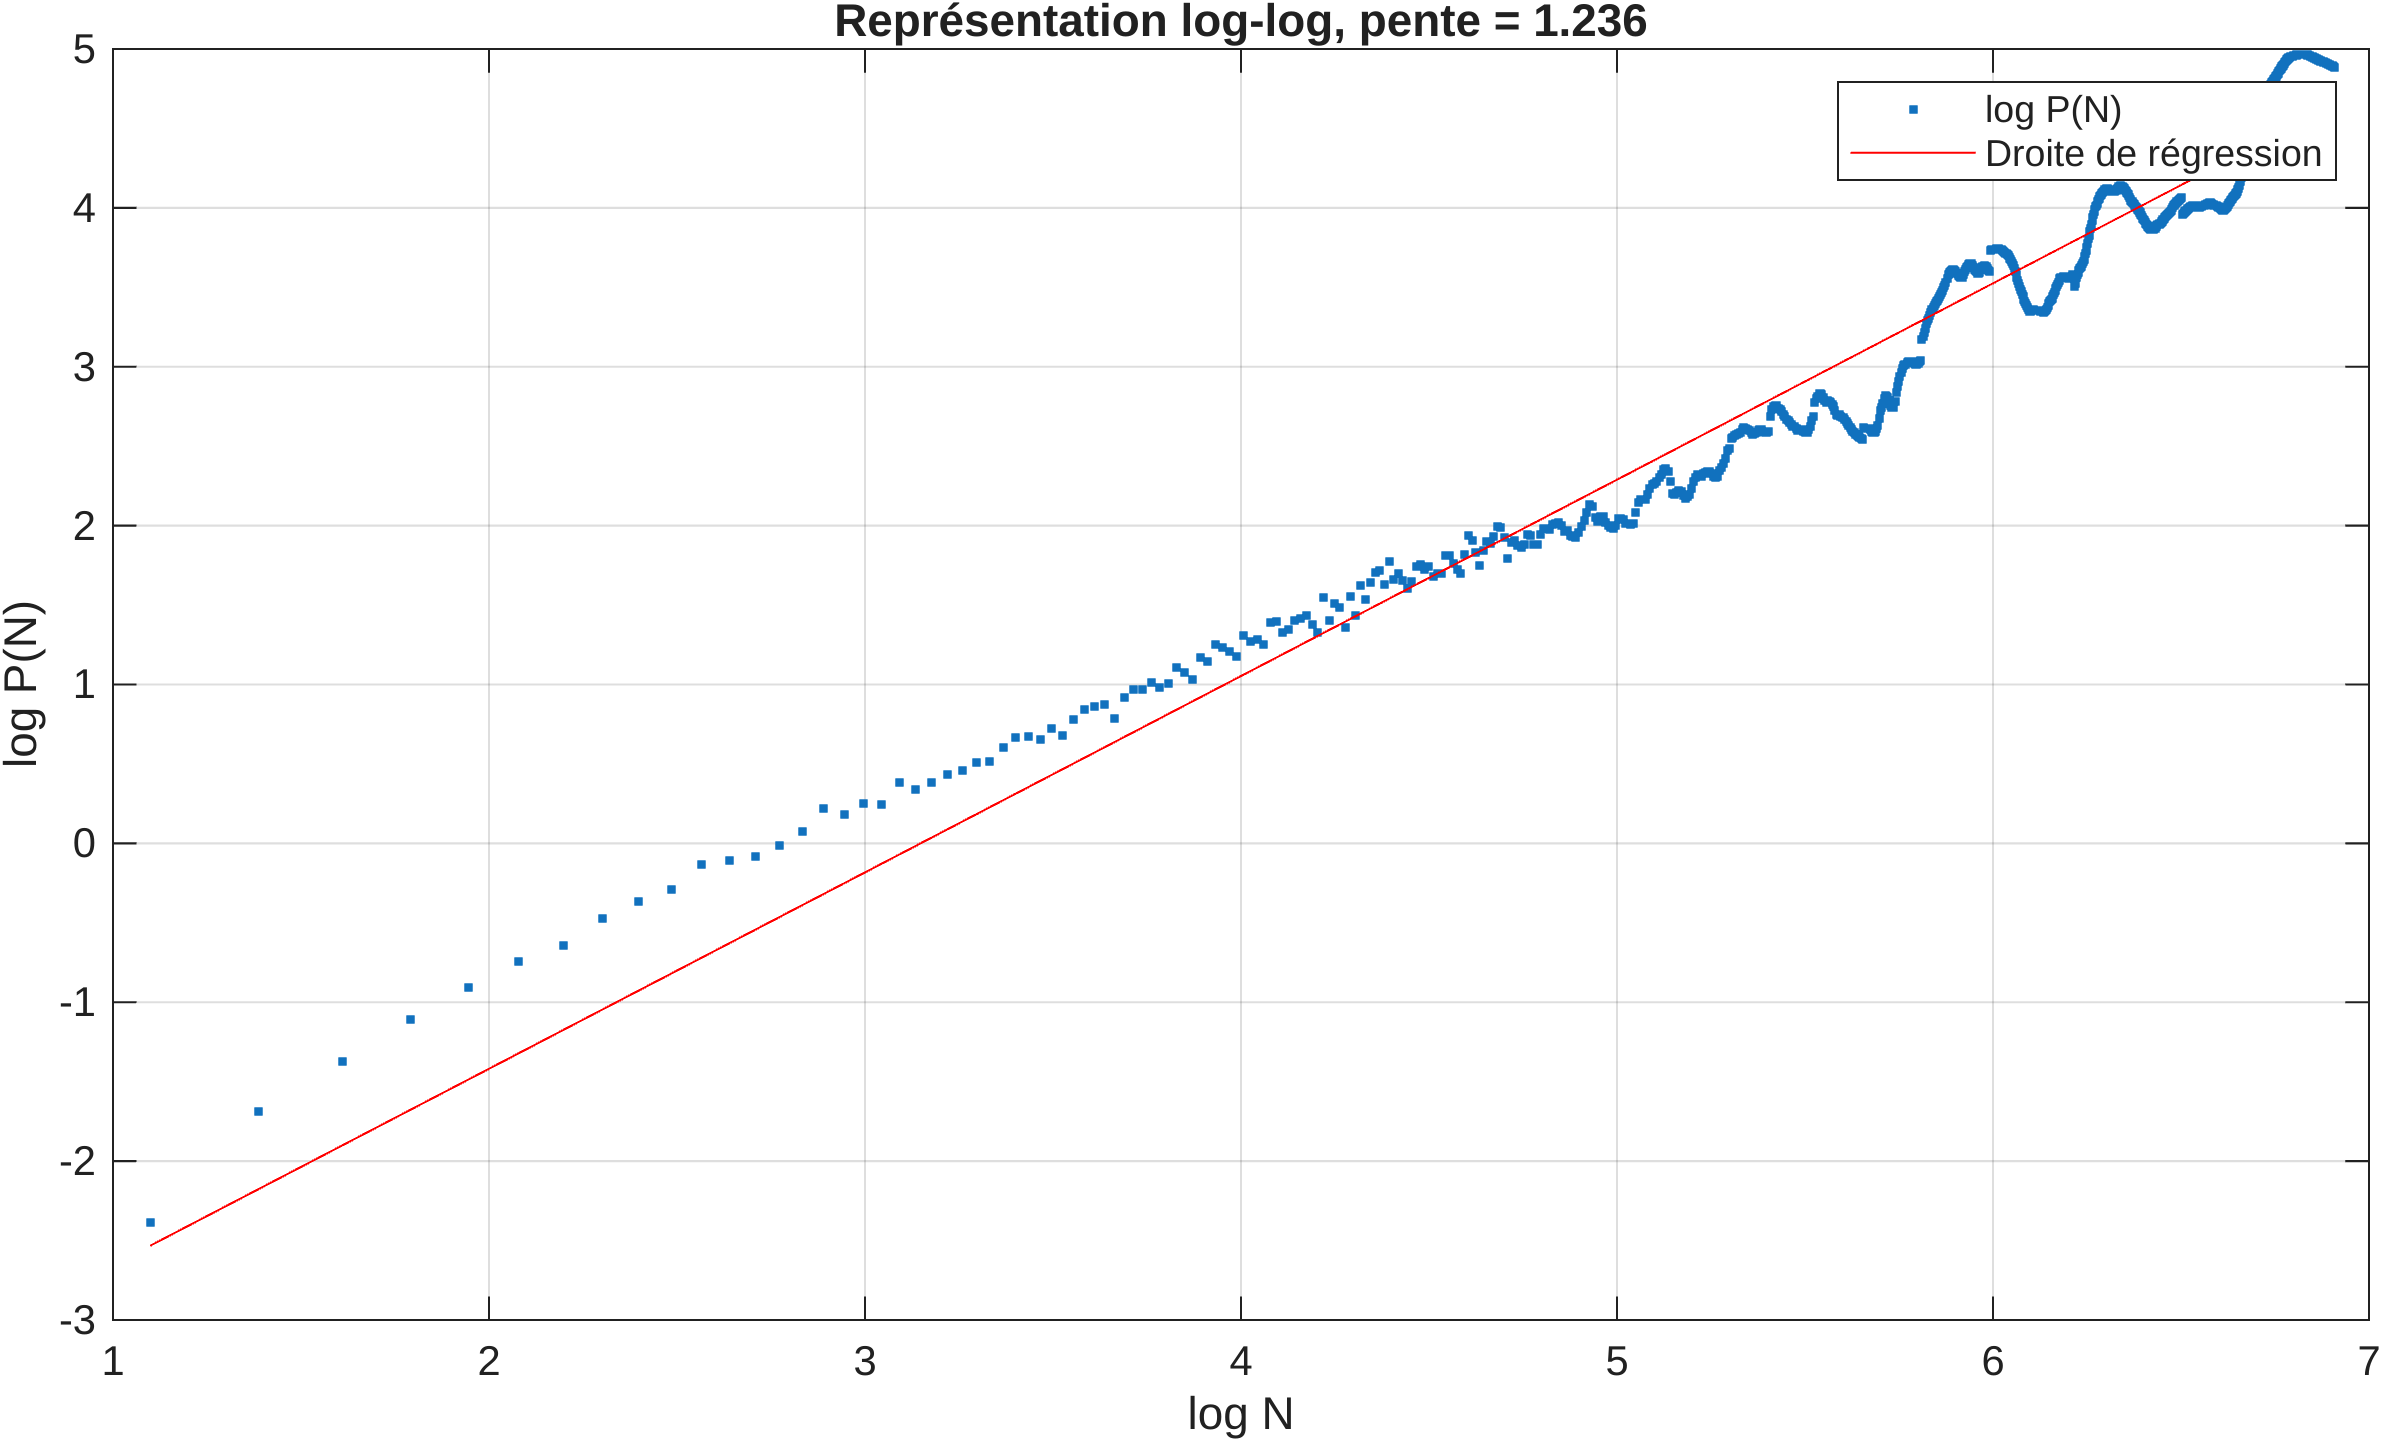
\includegraphics[width=0.5\linewidth]{fig19.png}
  \caption{Représentation log-log de $P(N)$ pour un bruit blanc intégré (tendance par droite) et droite de régression.}
  \label{fig:loglog}
\end{figure}

Sur la figure~\ref{fig:loglog}, la pente obtenue vaut $1{,}24$, pour une valeur attendue de 1. La lecture du graphique en donne la raison :
\begin{itemize}
  \item pour $2 < \ln N < 5$, c'est-à-dire $7 < N < 150$, les points sont bien alignés, avec une pente locale proche de 1 ;
  \item au-delà, le nuage oscille fortement. Pour ces valeurs, $P(N)$ n'est estimé que sur $L = \lfloor 2000/N \rfloor \leq 13$ blocs, et même sur 2 ou 3 blocs dès que $N > 500$.
\end{itemize}
Or, avec $N$ espacé linéairement, la moitié des 998 points de régression vérifie $N > M/4$. La régression est donc dominée par la zone la moins fiable, qui n'occupe qu'environ 12~\% de l'axe $\ln N$. Un échantillonnage logarithmique des valeurs de $N$, ou une limitation à $N \leq M/10$ (au moins 10 blocs), comme le recommande la littérature sur la DFA~[6], rendrait le marqueur plus robuste.

%=====================================================================
\section{Applications}
\label{sec:applications}
%=====================================================================

\subsection{Protocole}

La méthode est appliquée, avec $M = 2000$, à deux signaux :
\begin{itemize}
  \item \textbf{cas n°1}, un bruit blanc gaussien centré de variance unité ;
  \item \textbf{cas n°2}, un processus AR(2) défini par $A(z) = 1 - 1{,}5z^{-1} + 0{,}7z^{-2}$. Ses pôles ont un module $\sqrt{0{,}7} \approx 0{,}84$ et une fréquence $\pm 0{,}073$. Il s'agit d'une résonance basse fréquence, de pseudo-période d'environ 14 échantillons, et le temps de corrélation est de l'ordre de $1/(1-0{,}84) \approx 6$ échantillons.
\end{itemize}
La tendance est estimée par la méthode 2a pour $d = 0$ à 3, avec et sans l'intégration de l'étape~1. Pour chaque cas, la même réalisation est utilisée pour tous les degrés : les écarts entre lignes d'une même colonne du tableau~\ref{tab:pentes} ne proviennent donc que de la méthode d'estimation de la tendance.

\begin{table}[ht]
  \centering
  \begin{tabular}{ccccc}
    \toprule
    & \multicolumn{2}{c}{Avec intégration} & \multicolumn{2}{c}{Sans intégration} \\
    \cmidrule(lr){2-3} \cmidrule(lr){4-5}
    Degré $d$ & Bruit blanc & AR(2) & Bruit blanc & AR(2) \\
    \midrule
    0 (moyenne) & 0,58 & 0,77 & 0,02 & 0,05 \\
    1 (droite) & 0,84 & 0,83 & 0,03 & 0,14 \\
    2 & 0,93 & 0,79 & 0,05 & 0,21 \\
    3 & 0,93 & 0,93 & 0,06 & 0,26 \\
    \bottomrule
  \end{tabular}
  \caption{Marqueur (pente de $\ln P(N)$ en fonction de $\ln N$) pour $M = 2000$, $N$ de 3 à $M/2$.}
  \label{tab:pentes}
\end{table}

\subsection{Avec intégration}

Pour le bruit blanc, les pentes sont comprises entre $0{,}58$ et $0{,}93$, inférieures à la valeur théorique de 1. Elles restent toutefois compatibles avec la variabilité d'une réalisation à l'autre : la réalisation de la figure~\ref{fig:loglog} donnait $1{,}24$ pour $d = 1$, contre $0{,}84$ ici.

Le résultat marquant est que l'AR(2) donne des pentes voisines de celles du bruit blanc, entre $0{,}77$ et $0{,}93$. Ce processus est à mémoire courte : pour $N$ grand devant son temps de corrélation, les incréments de son profil sont quasiment décorrélés et le profil se comporte comme une marche aléatoire, avec $P(N) \propto N$. Le comportement spécifique de l'AR(2) ne concerne que les petites échelles, $N \lesssim 15$, soit une douzaine de points sur 998. Il est donc invisible dans la pente globale. Avec cette grille de $N$, le marqueur ne permet pas de distinguer les deux processus.

\subsection{Sans intégration}

En supprimant l'intégration, la méthode est appliquée directement au signal centré :
\begin{itemize}
  \item pour le bruit blanc, les pentes deviennent quasi nulles ($0{,}02$ à $0{,}06$). C'est ce que prévoit~\eqref{eq:PN_bb} : $P(N)$ est presque constant et ne s'en écarte que par le terme $(d+1)/N$, qui croît avec $d$. Cela explique la légère augmentation de la pente avec le degré ;
  \item pour l'AR(2), les pentes croissent nettement avec $d$, de $0{,}05$ à $0{,}26$. Pour les petits blocs, un polynôme de degré élevé suit les oscillations lentes de l'AR(2), de pseudo-période 14 échantillons, et absorbe une partie de sa puissance. $P(N)$ est alors réduit aux petites échelles, ce qui augmente la pente.
\end{itemize}
Sans intégration, le marqueur distingue donc le bruit blanc, avec une pente proche de 0, de l'AR(2), avec une pente nettement positive dès $d \geq 1$. C'est la situation inverse du cas intégré. L'intégration est ce qui donne au marqueur son interprétation en termes d'exposant $\alpha$, avec $a = 1$ pour un bruit blanc. Elle réduit en revanche l'écart entre processus à mémoire courte, qui se comportent tous comme des marches aléatoires aux grandes échelles.

\subsection{Dépendance vis-à-vis de l'estimation de la tendance}

Avec intégration, le degré $d$ modifie sensiblement la pente sur une même réalisation : de $0{,}58$ à $0{,}93$ pour le bruit blanc. La moyenne ($d = 0$), qui laisse dans le résidu la dérive du profil à l'intérieur de chaque bloc, donne la pente la plus éloignée de 1. Entre $d = 1$ et $d = 3$, les écarts ($0{,}84$ à $0{,}93$) sont du même ordre que la dispersion entre réalisations. Sans intégration, la dépendance au degré est au contraire systématique et prévisible par~\eqref{eq:PN_bb}. Le marqueur dépend donc de la méthode d'estimation de la tendance, et la méthode doit être fixée une fois pour toutes pour comparer des signaux entre eux.

Les méthodes 2b et 2c n'ont pas été utilisées pour calculer le marqueur. Pour 2b, le retard $(N-1)/2$ introduirait dans le résidu une erreur structurelle qui croît avec $N$. Pour 2c, les transitoires imposent d'écarter $2(N-1)$ échantillons, ce qui devient impossible lorsque $N$ approche $M/2$. Dans les deux cas, la grille de $N$ prévue par le sujet devrait être restreinte.

\subsection{Dépendance vis-à-vis du nombre d'échantillons et des valeurs de $N$}

Pour le bruit blanc intégré et $d = 1$, une réalisation par valeur de $M$ donne :

\begin{center}
  \begin{tabular}{ccccc}
    \toprule
    $M$ & 500 & 1000 & 2000 & 5000 \\
    \midrule
    Pente & 0,91 & 1,18 & 0,74 & 1,19 \\
    \bottomrule
  \end{tabular}
\end{center}

Les valeurs fluctuent autour de 1 avec un écart atteignant $\pm 0{,}25$, qui ne diminue pas lorsque $M$ augmente. Ce résultat contre-intuitif découle de l'analyse de la figure~\ref{fig:loglog} : augmenter $M$ augmente aussi $N_{\max} = M/2$, si bien qu'il subsiste toujours des valeurs de $N$ pour lesquelles $P(N)$ n'est estimé que sur 2 ou 3 blocs, et qu'elles représentent toujours la moitié des points de régression. La variance du marqueur est dominée par ces grandes échelles, et non par la durée du signal.

Le marqueur dépend donc fortement de la réalisation et des valeurs de $N$ retenues, ce qui constitue le principal obstacle à un usage en classification. Trois améliorations en découlent : échantillonner $N$ de manière logarithmique, pour que chaque échelle pèse autant dans la régression ; limiter $N$ à environ $M/10$, pour disposer d'au moins 10 blocs ; moyenner le marqueur sur plusieurs réalisations ou segments, avec un intervalle de confiance. Enfin, pour l'AR(2), une régression restreinte aux petites échelles ($N \lesssim 15$) ferait apparaître une pente différente de celle des grandes échelles : cette rupture de pente est elle-même une information discriminante, que la pente globale efface.

%=====================================================================
\section{Conclusion}
%=====================================================================

La première partie a caractérisé deux processus de référence : un MA(4), SSL, d'autocorrélation à support fini et de DSP à creux en $1/4$ et $4/9$, et un AR(4), asymptotiquement SSL, d'autocorrélation à décroissance géométrique et de DSP à résonances très fines en $1/3$ et $3/7$. Le périodogramme n'étant pas consistant, quatre estimateurs lissés ont été comparés. Le choix de leurs paramètres à partir de la largeur à mi-hauteur des structures spectrales a illustré le compromis biais-variance : la résolution requise par l'AR(4) limite la réduction de variance à un facteur 5 à 7. La fuite spectrale de la fenêtre rectangulaire domine dès que la dynamique est grande, ce qui fait du périodogramme de Welch avec fenêtre de Hann le meilleur compromis observé.

Pour la méthode, l'estimation de la tendance par blocs a été formalisée comme un problème de moindres carrés, dont la solution est une projection orthogonale. La moyenne glissante causale est un filtre RIF stable, à phase linéaire mais pas à minimum de phase, dont le retard de $(N-1)/2$ échantillons pénalise l'estimation. Des deux stratégies de filtrage à phase nulle, la première l'est pour tout $h$ réel, la seconde seulement si $\operatorname{Re}\{H\} \geq 0$.

Les applications confirment une pente voisine de 1 pour un bruit blanc intégré et voisine de 0 sans intégration. Elles montrent aussi les limites du marqueur : il dépend de l'estimation de la tendance, sa variabilité ne diminue pas avec $M$ car la régression est dominée par les grandes échelles, et, avec intégration, il ne distingue pas un AR(2) d'un bruit blanc. Un échantillonnage logarithmique des échelles et l'étude de la pente sur plusieurs plages d'échelles sont les prolongements naturels de ce travail, avant une application à des signaux réels.

%=====================================================================
\section{Organisation du projet}
%=====================================================================

Le projet s'est déroulé sur quatre séances encadrées, complétées par du travail personnel. Le code a été partagé au moyen d'un dépôt Git et le rapport rédigé en \LaTeX.

\begin{table}[ht]
  \centering
  \renewcommand{\arraystretch}{1.6}
  \begin{tabular}{|c|c|p{6.2cm}|c|c|}
    \hline
    Séance & Date & Tâches réalisées & M. Cirou (h) & M. Païtard (h) \\
    \hline
    1 & & & & \\
    \hline
    Entre 1 et 2 & & & & \\
    \hline
    2 & & & & \\
    \hline
    Entre 2 et 3 & & & & \\
    \hline
    3 & & & & \\
    \hline
    Entre 3 et 4 & & & & \\
    \hline
    4 & & & & \\
    \hline
    Après 4 & & & & \\
    \hline
    \textbf{Total} & & & & \\
    \hline
  \end{tabular}
  \caption{Répartition des tâches et temps passé par chacun.}
  \label{tab:organisation}
\end{table}

%=====================================================================
\section*{Références}
\addcontentsline{toc}{section}{Références}
%=====================================================================

\begin{enumerate}
  \renewcommand{\labelenumi}{[\arabic{enumi}]}
  \item P. D. Welch, « The use of fast Fourier transform for the estimation of power spectra: a method based on time averaging over short, modified periodograms », \emph{IEEE Transactions on Audio and Electroacoustics}, vol. 15, n°2, p. 70--73, 1967.
  \item M. S. Bartlett, « Smoothing periodograms from time series with continuous spectra », \emph{Nature}, vol. 161, p. 686--687, 1948.
  \item R. B. Blackman, J. W. Tukey, \emph{The Measurement of Power Spectra}, Dover, 1958.
  \item F. J. Harris, « On the use of windows for harmonic analysis with the discrete Fourier transform », \emph{Proceedings of the IEEE}, vol. 66, n°1, p. 51--83, 1978.
  \item C.-K. Peng, S. V. Buldyrev, S. Havlin, M. Simons, H. E. Stanley, A. L. Goldberger, « Mosaic organization of DNA nucleotides », \emph{Physical Review E}, vol. 49, p. 1685--1689, 1994.
  \item J. W. Kantelhardt, E. Koscielny-Bunde, H. H. A. Rego, S. Havlin, A. Bunde, « Detecting long-range correlations with detrended fluctuation analysis », \emph{Physica A}, vol. 295, p. 441--454, 2001.
\end{enumerate}

%=====================================================================
\section*{Annexe : codes MATLAB}
\addcontentsline{toc}{section}{Annexe : codes MATLAB}
%=====================================================================

L'ensemble des codes MATLAB est fourni avec le rapport. Le script principal \texttt{Prj\_2\_2.m} reproduit toutes les figures présentées et affiche dans la console les marqueurs du tableau~\ref{tab:pentes}. Il s'appuie sur trois fonctions, dont l'en-tête précise les entrées, les sorties et l'objet :
\begin{itemize}
  \item \texttt{pDaniell} calcule le périodogramme de Daniell ;
  \item \texttt{pWelchMain} calcule le périodogramme de Welch, ou celui de Bartlett lorsque la fenêtre est rectangulaire et le recouvrement nul ;
  \item \texttt{marqueur} enchaîne les étapes 1 à 4 de la méthode pour un degré de tendance donné.
\end{itemize}

\vfill
\noindent\textit{Rapport réalisé en collaboration avec Claude (Anthropic).}

\end{document}
